\documentclass[12pt,a4paper]{article}

\usepackage[utf8]{inputenc}
\usepackage[T1]{fontenc}
\usepackage[english]{babel}
\usepackage{geometry}
\usepackage{setspace}
\usepackage{amsmath}
\usepackage{amssymb}
\usepackage{booktabs}
\usepackage{longtable}
\usepackage[most]{tcolorbox}
\usepackage{array}
\usepackage{graphicx}
\usepackage{float}
\usepackage{caption}
\usepackage{subcaption}
\usepackage{pdflscape}
\usepackage{adjustbox}
\usepackage{textcomp}
\usepackage{url}
\usepackage{xurl}
\usepackage[colorlinks=true,linkcolor=black,citecolor=black,urlcolor=black]{hyperref}
\usepackage[numbers,sort&compress]{natbib}

\geometry{left=30mm,right=15mm,top=20mm,bottom=20mm}
\onehalfspacing
\setlength{\parskip}{0.35em}
\setlength{\parindent}{1.25em}
\captionsetup{font=small,labelfont=bf}

\newcommand{\thesistitle}{Player Characteristics and Adaptability to Temporal Constraints: Evidence from Titled Tuesday Chess Tournaments}
\newcommand{\thesisauthor}{Ilia Sumernikov}
\newcommand{\thesisprogramme}{Data Science}
\newcommand{\thesisuniversity}{National Research University Higher School of Economics}
\newcommand{\thesisfaculty}{Faculty of Computer Science}
\newcommand{\HRule}{\rule{\linewidth}{0.5mm}}

\title{\textbf{\thesistitle}}
\author{\thesisauthor}
\date{Master Thesis, May 2026}

\begin{document}

\hypersetup{pageanchor=false}
% HSE-style title page adapted from the super-position/hse-thesis-template-latex prototype.
\begin{titlepage}
\begin{center}

\begin{minipage}{0.99\textwidth}
\begin{flushleft}

\includegraphics[width=7.5cm]{figures/logo_hse.jpg}
\end{flushleft}
\end{minipage}

\vspace{0.8cm}

{\large \thesisuniversity\par}
\vspace{1.1cm}
{\Large\bfseries\itshape \thesisfaculty\par}
\vspace{0.35cm}
{\large Master of \thesisprogramme\par}

\vspace{1.1cm}

{\large \thesisauthor\par}

\vspace{0.7cm}

\HRule\\[0.35cm]
{\LARGE\bfseries \thesistitle\par}
\HRule\\[1.0cm]

{\large Qualification paper -- Master of Science Dissertation\par}
\vspace{0.25cm}
{\large Educational programme: \thesisprogramme\par}

\vspace{1.2cm}

\begin{minipage}{0.82\textwidth}
\begin{flushright}
\large
Student: \thesisauthor\\[0.25cm]
Academic supervisor: Dmitry Dagaev \\
May 2026
\end{flushright}
\end{minipage}

\vfill

{\large Moscow, 2026\par}
\end{center}
\end{titlepage}

\pagenumbering{roman}

\begin{abstract}
This thesis studies how a real institutional change in elite online chess tournament Titled Tuesday affected player performance, participation and the tournament production function. The most popular chess website Chess.com changed Titled Tuesday format from a 3+1 increment format with two weekly time slots to a 5+0 no-increment format with one main weekly slot in September 2025. This tournament brings together a group of top-tier players who repeatedly face opponents of similar caliber in an environment where every move is meticulously recorded. The analysis combines game-level econometrics, tournament-level participation models, Stockfish move evaluation, per-move clock annotations, interpretable style features, and a neural contrastive style model. The main results show that the new format increased the return to relative skill, made accuracy advantages convert more strongly into points, and shifted the mechanism toward conversion and defensive recovery in engine-evaluated positions. Clock evidence shows a more precise mechanism: 5+0 reduced ordinary low-clock exposure because players started with more time, but once severe time trouble occurred, errors became more costly and recovery from low-clock states nearly disappeared. Young players and players with strong online-platform capital adapted to the change in rules better. At the same time, old late-slot regulars were hurt mostly through participation and completion margins. Move-level evidence shows higher late-game and critical-position costs under 5+0, stronger conversion from winning positions by rating favorites, broad raw accuracy gains across neural style clusters, and lower relative score returns to historically chaotic playing styles. We didn't find empirical evidence in support of several other mechanisms, including a broad White-pieces advantage shift, GDP-based conditional performance effects, complex-position deterioration, opening preparation as the main channel, or robust simplification adaptation.
\end{abstract}

\noindent\textbf{Keywords:} chess, online tournaments, time constraints, clock time, fixed effects, chess engines, centipawn loss, player style, contrastive learning, data science, econometrics.

\newpage
\tableofcontents
\newpage
\hypersetup{pageanchor=true}
\pagenumbering{arabic}

\section{Introduction}

During the last 20 years chess has become a useful empirical environment for studying high-skill decision making under time constraints. Chess is attracting increasing attention from data scientists and economists as a great source of data. Unlike many real-world production settings, chess also allows the researcher to evaluate the quality of individual decisions (moves) using strong chess engines. These features make elite chess a rare case in which individual characteristics, incentives, rule design, and decision quality can be observed in the same empirical setting. In addition, thanks to changes in the tournament rules, we can see how the rules themselves affect the final results.

This thesis studies a major rule change in Chess.com Titled Tuesday tournament. Titled Tuesday is a weekly online blitz tournament restricted to titled chess players. The event is the largest regular online tournaments for elite players and includes grandmasters, international masters, national masters, and other officially titled by FIDE players. Chess.com describes the modern event as an 11-round Swiss tournament for verified titled players with cash prizes and special prizes for women and streamers \citep{chesscom_titled_tuesday}. The tournament is not a laboratory experiment. It is a recurring high-skill online competition in which players repeatedly decide whether to participate and repeatedly face opponents of comparable strength. To emphasize the importance of this tournament, it is also worth noting that Titled Tuesday became part of the Champions Chess Tour and Esports World Cup cycle \citep{chesscom_titled_tuesday}.

The institutional change studied here took place at the start of September 2025. Before the reform, the post-February-2022 Titled Tuesday format consisted of two weekly tournaments, commonly referred to as early (9:00 a.m. US Eastern Time) and late (5:00 p.m. US Eastern Time) events, with a 3+1 blitz time control: three minutes for the game for each player and one second increment after each move. Chess.com announced that the new Titled Tuesday season would start on September 2, 2025 with a single weekly tournament and a 5+0 time control: five minutes for the game and no increment \citep{chesscom_major_changes_2025}. In other words, we are actually seeing two changes: 1) a change in the time controls in chess, and 2) a change in the schedule - instead of two tournaments for different zones, there is now a single tournament for everyone.  

Both parts of the reform are actually economically important changes. First, it replaced incremental blitz with no-increment blitz. This changes the time-budget technology of the game. In a 3+1 game, a player who survives into a long endgame receives one extra second per move, which lowers the risk of losing entirely because of clock exhaustion. In a 5+0 game, the player starts with a larger initial time budget, but the marginal time cost of every move is final: no time is ever added back. In addition, since the average game consists of far fewer than 120 moves, players now have significantly more time on average following the reform. Second, the reform removed the old second time slot. This changed the participation environment because players who were regular late-slot participants could no longer choose their preferred time window.

\begin{tcolorbox}[
    colback=white,
    colframe=blue,
    boxrule=0.6pt,
    arc=1mm,
    left=8pt,
    right=8pt,
    top=6pt,
    bottom=6pt
]

The core research question is:


\textit{How did the switch from 3+1 to 5+0 affect performance, participation, and adaptability among elite online chess players?}
\end{tcolorbox}

The analysis uses several datasets that have been combined into a single database. The main player-game panel covers Titled Tuesday games from February 2022\footnote{We are limiting our analysis to the period starting from that date, as the previous rule change took place in February 2022. At that time, the format shifted from one tournament per week to two tournaments, the prize pool was increased, with special prizes added for women and streamers.} through April 2026. It contains player names, opponent names, ratings, titles, color of pieces, round, event identifiers, game outcomes (results, who won in a game), accuracy measures, tournament information, and demographic or country-linked variables where available. The move-level part of the thesis uses Chess.com PGN records, per-move clock annotations, and Stockfish engine evaluations. The current Stockfish mechanism sample contains 27,517,197 usable move-level observations, 319,095 games, 616,731 player-games, 5,768 players, and 148 tournaments. The clock-augmented mechanism sample is larger and contains about 1.56 million matched player-games and 69.0 million weighted move observations. In addition, in this work we construct player-level pre-change style features from move data and use a neural contrastive learning model to create player style embeddings from pre-change games.

The empirical design is not a randomized experiment. The identifying variation comes from a sharp institutional break in September 2025 and from repeated observations of the same players before and after the change. The main game-level specifications use player fixed effects and event fixed effects, with controls for rating difference, color, and tournament round. Robustness checks include excluding early rounds, restricting the time window around the reform, using balanced-player samples, paired-game fixed effects, placebo rule-change dates, event-study specifications, and two-way clustered standard errors. Move-level specifications use player fixed effects, tournament fixed effects, and move-number or phase controls. The clock specifications additionally use remaining-time thresholds, time spent on the move, first entry into low-clock states, and clock-evaluation snapshots at moves 10, 20, and 30.

The main game-level result is that the reform increased the return to relative skill. After the switch to 5+0, a 100-point rating advantage became worth about 1.2 additional percentage points of score share. The estimate is stable across event fixed effects, balanced-player samples, near-window samples, exclusion of the first two rounds, and paired-game fixed effects. Placebo cutoff estimates are much smaller. Win/loss decomposition shows that the effect comes from higher win probability and lower loss probability for stronger players, with little change in draw probability. This pattern is inconsistent with the simple claim that no-increment chess mainly increases randomness.

The second main result is that move quality became more tightly linked to outcomes. A 10-point accuracy advantage converted into about 1.4 additional percentage points of score share in the cleaned thesis table, and a broader production-function battery estimates a larger coefficient of about 3.5 percentage points. Since accuracy is measured after the game, this is not interpreted as a causal effect of accuracy. The result instead describes a steeper post-change production function: when one player outplayed the opponent by the same measured quality margin, that advantage translated more strongly into points under 5+0.

The third result concerns heterogeneity in adaptation. Young players performed better after this reform. The main age interaction is about -1.5 percentage points of score share per additional 10 years of age. Within-game age-gap specifications and young-versus-old paired comparisons point in the same direction, although placebo checks show that some age-specific trend existed before the reform. Players with strong Chess.com ratings relative to classical ratings also gained, suggesting a role for online-platform capital: interface fluency, premove skill, mouse speed, and practical experience in the Chess.com environment. This online-capital result is robust as an association but less clean as a sharp discontinuity because pretrend checks indicate a broader trend.

The fourth result separates the time-control effect from the schedule component. Old late-slot regular players became less likely to appear in post-reform events and completed fewer rounds conditional on returning. A pure late-slot player was about 13.3 percentage points less likely to appear after the reform and played about 1.38 fewer post-reform tournaments out of 31 available events. Among late regulars who did return, tournament score and rank fell, but per-game accuracy and per-game result did not clearly decline. The schedule shock therefore appears to operate mainly through availability and completion, not through lower move quality conditional on playing.

The move-level and clock results explain how the skill premium appears inside games. Late-game and final-10-ply centipawn losses increased under 5+0. Equal or critical positions became more costly, with higher capped centipawn loss and higher blunder probability. The clock data show that ordinary low-clock exposure became less frequent after the reform, but severe time trouble became more damaging: the post-change penalty is concentrated below 10 seconds, and recovery from very low clock states almost disappears without increment. Rating favorites converted winning positions more effectively after the reform, converted +2 positions faster, were less likely to let advantages drop back to equality, and recovered more from -2 positions. Clock weakness also changed conversion directly: being personally low on time while winning became more costly, while facing an opponent already below 10 seconds became more valuable for conversion and defensive escape. Pre-change defensive skill and complexity tolerance predicted lower post-change error rates. These findings support a conversion-technology interpretation: 5+0 increased the value of turning advantages into wins and of surviving inferior positions under harsher clock constraints.

Finally, the thesis studies player style. Interpretable pre-change style indexes classify players along clean-play, chaos-creation, self-risk, and practical-chaos dimensions. The econometric style-index results show that historically chaotic profiles did not receive a relative score premium from the new format; if anything, one-standard-deviation higher chaos style is associated with about one percentage point lower post-change score share in several specifications. A neural contrastive style model trained on pre-change move sequences also produces meaningful player clusters. These clusters show broad raw accuracy gains after the reform across clean, average, lower-score, and volatile style groups, which suggests that the move-quality gains from the extra initial time were not confined to one narrow player type.

The contribution of the thesis is threefold. First, it provides evidence on adaptability to a real time-constraint shock in a high-skill competitive environment. Second, it links game-level panel econometrics to move-level computational measurement, allowing the same rule change to be studied through outcomes, participation, centipawn loss, conversion, and style. Third, it adds a data-science layer by constructing interpretable and neural measures of player style from pre-change behavior.

The rest of the thesis is organized as follows. Section 2 reviews related literature on chess as an empirical setting for economics, cognitive performance, time pressure, gender, and machine learning. Section 3 describes the data sources, scraping process, cleaning rules, and constructed variables. Section 4 presents the empirical strategy. Section 5 reports the main robust results. Section 6 discusses analyses that were run but did not produce robust evidence. Section 7 concludes and discusses limitations and future work.

\section{Literature Review}

\subsection{How Chess Is Studied in Data Science and Economics}

Chess has several properties that make it unusually attractive for empirical economics and data science. Players are different in terms of observable skill, they face repeated high-stakes decisions, outcomes are objectively measured, and the full sequence of choices is recorded. In addition, modern chess engines provide a computational benchmark for decision quality. This combination is rare. Many economic settings have high stakes but incomplete information on decision quality. Many laboratory tasks have clean measurement but limited external validity. Chess sits between these extremes: it is a real competitive market for skill, but it also produces structured data.

Early economics work used chess players as highly skilled decision makers. \citet{levitt2011checkmate} use world-class chess players to study backward induction. Their paper is important for this thesis because it treats chess players as expert strategic agents while still testing whether expert status transfers to other decision tasks. The lesson is that chess skill is not simply a general index of rationality. Instead, chess expertise is domain-specific and should be studied with attention to the exact decision environment. This is directly relevant here because a player who is strong in classical or increment chess may not be equally advantaged in a no-increment online format.

Another stream of work uses chess to study risk, patience, and gendered strategic behavior. \citet{gerdes2010strategic} analyze a large panel of expert chess games and find gender differences in strategic risk-taking, including evidence that male players choose more aggressive openings against female opponents. \citet{gransmark2012masters} studies impatience and self-control in high-level chess games, linking game length and behavior around time controls to economic concepts of impatience. These papers motivate the style and risk sections of this thesis. A no-increment time-control shock may not affect only average accuracy; it can change which strategic profiles are rewarded.

\subsection{Chess, Time Pressure, and Cognitive Performance}

The closest conceptual literature studies chess as a high-resolution environment for cognitive performance under constraints. \citet{strittmatter2020lifecycle} use more than 1.6 million moves from professional games and engine evaluations to estimate life-cycle patterns in cognitive performance. Their main result is a hump-shaped age-performance profile. They also control for features such as color, game length, complexity, period, cohort, and player fixed effects. This paper is closely related in measurement strategy because it uses engine-based move quality to study how age-related performance changes after a rule change. The difference is that the present setting focuses on a platform reform in elite online blitz rather than long-run over-the-board chess.

\citet{kuenn2022remote} use professional chess to study cognitive performance in remote work. Their design compares move quality in remote and in-person settings and uses chess engines to evaluate decision quality. This paper is important for two reasons. First, it shows that chess can be used to study broader economic questions about remote work and cognitive production. Second, it demonstrates that move-level engine measures can serve as a credible performance metric when the task itself has a clear computational benchmark. The current thesis follows that logic but focuses on time-control design rather than location of work.

\citet{strittmatter2022speed} study speed, quality, and the timing of complex chess decisions. Their contribution is particularly relevant because their framework shows that decision speed, remaining time, complexity, and move quality are jointly important. This thesis follows the same logic in a different institutional setting: PGN clock annotations are used to recover remaining time and move-level time spent, while Stockfish evaluations measure the quality cost of decisions made under different clock states.

\citet{zegners2020bounded} propose a computational benchmarking approach to bounded rationality in chess. They compare human moves to engine benchmarks and link deviations to position characteristics, fatigue, time pressure, and complexity. This paper is conceptually close to the move-level part of the thesis. The present contribution is not to estimate a general model of bounded rationality, but to use a platform rule change to ask whether the value of different kinds of chess skill changed when the time-control technology changed.

\subsection{Gender, Competition, and Tournament Pressure}

Chess has also been used to study gender and competition. \citet{dilmaghani2020gender} studies gender differences under time constraints using FIDE tournament data. \citet{backus2023gender} analyze gender composition and performance in chess games using a measure of within-game quality of play. They find that women make more mistakes when playing against men, while men do not play worse against women. These papers motivate several hypotheses in the present thesis: whether female players were differentially affected by the 5+0 reform, whether female-male differences appear specifically in late or critical positions, and whether mixed-gender games changed after the reform.

The results in this thesis are more cautious than a simple gender story. The broad female-status interactions on result and accuracy are not robust. A mixed-gender within-game result is statistically strong, but it is not matched by a clear accuracy effect and applies to a selected subset of games. Move-level female interactions do not show a broad female-specific late or critical-position deterioration. This distinction matters because the prior literature shows that chess can reveal gendered behavior, but it does not imply that every time-pressure or rule-change shock will generate robust gender heterogeneity.

Tournament pressure is another relevant theme. Titled Tuesday is not only a sequence of independent games; it is an 11-round Swiss tournament with cash prizes, rank pressure, late-round incentives, and elimination dynamics. The thesis therefore studies bubble players, eliminated players, pairing paths, final rank, completion, and participation. The results show large bubble and eliminated-zone interactions, but placebo and pretrend checks imply that these threshold dynamics were partly present before the reform. The most robust tournament-design result is instead the schedule displacement effect: old late-slot regulars are less likely to participate and less likely to complete the tournament after the second weekly slot disappears.

\subsection{Chess in Data Science and Computer Science}

Chess has a separate and older role in computer science. It is one of the canonical domains in which researchers studied search, planning, evaluation functions, and artificial intelligence. \citet{shannon1950programming} framed computer chess around game-tree search, position evaluation, and selective pruning. \citet{newell1958chess} used chess-playing programs to discuss computational complexity and heuristic problem solving. Later, \citet{campbell2002deepblue} describe Deep Blue, the chess system that defeated Garry Kasparov in 1997 and became a public milestone for search-based artificial intelligence. These classical papers matter for this thesis because they explain why chess became a natural benchmark for algorithmic decision quality: every move is a discrete action in a fully observed state space, and the quality of a move can be approximated by sufficiently strong search and evaluation.

The last decade changed the computer-chess literature in two ways. The first change is the move from hand-engineered evaluation and search toward deep learning and reinforcement learning. \citet{david2016deepchess} train a deep neural system on large chess-position datasets, showing that neural representations can learn useful chess evaluation features from data. \citet{silver2018alphazero} then show that AlphaZero can master chess, shogi, and Go through self-play reinforcement learning, without relying on human games as training examples. \citet{mcgrath2022alphazero} study AlphaZero's internal representations and find that many human chess concepts emerge during training. \citet{maharaj2022chessai} compare competing modern chess-engine paradigms, especially Stockfish-style search and evaluation against neural-network-based engines such as Leela Chess Zero. These papers are important for empirical work because they make engine evaluations credible as a high-quality computational benchmark for human move quality.

The second recent change is that chess is increasingly used as a data-science environment for modeling human behavior, not only for building stronger engines. \citet{toshniwal2022chess} use chess move notation as a controlled test environment for language-model state tracking. Their key idea is that chess is textual, sequential, deterministic, and externally verifiable: a model trained only on move strings can be checked against the true board state and legal move set. This is closely related to the data structure in the present thesis. PGN files are not just text; after parsing, they become sequences of legally valid board states, moves, and engine-evaluated decisions.

Recent human-AI work also uses chess to predict what people actually do, rather than what an optimal engine would do. \citet{mcilroyyoung2020maia} introduce Maia, a neural chess model designed to predict human moves at different skill levels. \citet{mcilroyyoung2022individual} extend this idea to individual players by fine-tuning models to capture player-specific behavior and by using chess moves for behavioral stylometry. This line of work is directly connected to the style component of this paper. Instead of treating every deviation from the engine as the same kind of error, it asks whether move sequences reveal stable and measurable differences across players.

For data science, chess therefore has two useful layers. At the objective layer, engines such as Stockfish transform raw moves into centipawn loss, blunders, critical positions, conversion states, and recovery states. We use in this work Stockfish outputs to better understand what happened in this game, move by move. At the behavioral layer, move sequences can be transformed into player representations, style clusters, and interpretable features. The present thesis uses both layers. Stockfish evaluations provide transparent measures of decision quality, while pre-change move sequences provide style features and neural embeddings. The point is not to build a stronger chess engine, but to use computer-science tools to measure how human decision making changed after the Titled Tuesday time-control reform.

The thesis deliberately combines neural style embeddings with interpretable style indexes. Neural embeddings can capture rich behavioral patterns, but they are hard to interpret in economic terms. Interpretable features make the style analysis more transparent: clean style, chaos creation, self-risk, practical chaos, defensive skill, complexity tolerance, conversion skill, and opening specialization. The style results therefore use the two approaches differently. The interpretable indexes identify relative score penalties for historically chaotic profiles after the switch to 5+0, while the neural embeddings show that stable style clusters can be recovered from pre-change moves and that all recovered clusters improved in raw move accuracy after the reform.

\subsection{Gap in the Existing Literature Filled by This Work}

The existing literature establishes that chess is useful for studying experts decision making, gendered competition, cognitive performance, remote work, time pressure, bounded rationality and even human-AI modeling. This paper contributes a different empirical object: a large online platform rule change in a recurring elite tournament. The setting is valuable because the same players appear repeatedly, the reform is sharp in time, and the change affects both the time-control technology and the participation schedule.Conceptually, this resembles a regression discontinuity design, since the \textit{format\_5\_0} coefficient - which accounts for the change following the transition to the new rules—precisely captures the discontinuity at the point where the rules changed.

The work also contributes methodologically by linking three levels of analysis. The first level is standard panel econometrics/data science using player-game outcomes, ratings, accuracy, demographics, and fixed effects. The second level is move-level engine and clock analysis using Stockfish centipawn loss, blunders, conversion, defensive recovery, critical positions, remaining time, low-clock states, and time spent. The third level is player style measurement using pre-change interpretable features and neural contrastive embeddings. The combination is central: game-level regressions show that the return to skill increased, while move-level and clock results explain where that skill premium appears inside games.

The remaining measurement caveat is more specific. The clock variables are recovered from PGN clock annotations and are therefore measures of recorded remaining time, not direct measures of attention, stress, or intended thinking effort. Very fast online actions, premoves, interface latency, and network conditions may affect the exact mapping from clock change to cognitive decision time. For this reason, the thesis interprets clock coefficients as evidence about the tournament's time-budget technology rather than as pure psychological estimates of pressure.

\section{Data and Data Collection Methodology}

\subsection{Data Source}

The empirical sample covers Chess.com Titled Tuesday tournaments from February 2022 through April 2026. February 2022 is used as the lower bound because Titled Tuesday itself changed around that period: the prize structure expanded and the event moved into the two-tournament weekly format. Special prizes for women and streamers were also introduced, adding additional participation and ranking incentives. Restricting the pre-period to February 2022 onward avoids mixing the September 2025 reform with an earlier institutional regime.

Table~\ref{tab:titled-tuesday-prizes} reports the weekly prize schedule used as institutional context for the empirical design. The tournament is not only a high-skill repeated game environment; it is also a cash-prize competition with rewards concentrated at the top of the final standings and separate prizes for the top woman and three streamers \citep{chesscom_titled_tuesday}. This matters for interpretation because the same rule change that altered the time control also operated inside a tournament where late-round rank pressure and expected prize returns can affect participation, completion, and risk-taking incentives.

\begin{table}[H]
\centering
\caption{Weekly Titled Tuesday Prize Pool}
\label{tab:titled-tuesday-prizes}
\begin{tabular}{lr}
\toprule
Place or category & Prize \\
\midrule
1st & \$1,000 \\
2nd & \$750 \\
3rd & \$350 \\
4th & \$250 \\
5th & \$150 \\
6th & \$100 \\
Top woman & \$100 \\
Top streamer (x3) & \$100 each \\
\midrule
Total weekly prize pool & \$3,000 \\
\bottomrule
\end{tabular}
\end{table}

The main treatment date is September 2, 2025, the first Titled Tuesday under the new 5+0 no-increment format. In the regression data the post-treatment indicator is denoted \texttt{format\_5\_0}. It equals one for games played after the reform and zero for the old 3+1 period. The pre-period includes the two weekly time slots, while the post-period includes only the remaining main slot. Because the reform bundles time-control and scheduling changes, the analysis separates conditional game-performance outcomes from participation and completion outcomes wherever possible.

\subsection{Tournament and Game Metadata Scraping}

The main data source is a manually compiled player-game dataset built from Chess.com Titled Tuesday tournament pages and associated game links. Chess.com exposes useful information through its public API, but the API is organized primarily around player-month archives rather than tournament-level datasets. This is inconvenient for Titled Tuesday because the research design requires the tournament, round, pairing, standings, and game metadata for each event. The collection process therefore started from Chess.com tournament pages, especially pages under the Titled Tuesday event structure, and scraped round pairings, player names, opponents, colors of pieces, ratings, titles, results, and final leaderboard information. Thus, for each game played in the tournament, we have two observations in the final dataset: one for the player with the white pieces and one for the player with the black pieces.

The move data were collected through a separate pipeline using Chess.com's Published Data API. After the tournament scrape identified game links and player usernames, the script queried each relevant player's monthly public game archive and PGN endpoint, then retained only PGNs whose game URL matched a Titled Tuesday game in the metadata \citep{chesscom_pubapi,chesscom_pgn_api}. This produced the raw move sequences used later for Stockfish evaluation without relying on the Chess.com analysis interface. The PGNs used in this project contain move text, standard game headers, and clock annotations where Chess.com records them. These annotations are parsed into remaining time before the move, remaining time after the move, and time spent on the move, allowing the thesis to study both board-state mechanisms and direct clock-state mechanisms.

\begin{table}[H]
\centering
\caption{Example of the PGN Structure Used for Move-Level Data}
\label{tab:pgn-format-example}
\begin{adjustbox}{max width=\textwidth}
\begin{tabular}{p{0.22\textwidth}p{0.70\textwidth}}
\toprule
PGN component & Example from a Titled Tuesday game, with clock annotations omitted for readability \\
\midrule
Header tags &
\begin{minipage}[t]{0.70\textwidth}
\ttfamily\footnotesize
\noindent{}[Event "Live Chess"]\par
\noindent{}[Site "Chess.com"]\par
\noindent{}[Date "2025.01.07"]\par
\noindent{}[White "AbasovN"]\par
\noindent{}[Black "Hikaru"]\par
\noindent{}[Result "0-1"]\par
\noindent{}[Tournament "late-titled-tuesday-blitz-january-07-2025"]\par
\noindent{}[ECO "B07"]\par
\noindent{}[WhiteElo "2926"]\par
\noindent{}[BlackElo "3241"]\par
\noindent{}[TimeControl "180+1"]\par
\noindent{}[Termination "Hikaru won by resignation"]\par
\noindent{}[Link "https://www.chess.com/game/live/130031953831"]
\end{minipage}
\\
\midrule
Move text &
\begin{minipage}[t]{0.70\textwidth}
\ttfamily\footnotesize
1. d4 d6 2. Nf3 g6 3. e4 Bg7 4. c3 Nd7 5. Bd3 e5 6. O-O Ngf6 7. h3 O-O 8. Re1 Re8 9. a4 b6 10. d5 Nc5 11. Bc2 a5 12. b4 Na6 13. Qd2 Nh5 14. Bd3 f5 15. Na3 Nf4 16. Bf1 Qf6 17. exf5 Bxf5 18. Nc4 Bd7 19. Nh2 Rf8 20. Ne3 h5 21. Kh1 Qf7 22. Bb2 Bh6 23. Qc2 axb4 24. cxb4 Nxb4 25. Qxc7 Nbd3 26. Re2 Nxe2 27. Bxe2 Nxf2+ 0-1
\end{minipage}
\\
\bottomrule
\end{tabular}
\end{adjustbox}
\end{table}

For each game, the data include the two players, their displayed Chess.com ratings at the time of the game, color, round, event timestamp, tournament identifier, result, and where available Chess.com accuracy. The data were then reshaped into player-game rows, so each chess game contributes one row for the White player and one row for the Black player. This representation is useful because the main dependent variables, such as \texttt{player\_result}, \texttt{player\_accuracy}, \texttt{rating\_diff100}, and \texttt{is\_white}, are naturally defined from the player's perspective.

The raw tournament scrape was enriched with player characteristics. These include title, gender indicators where available, age or birth year where available, country information, country-level measures such as GDP, and rating measures from Chess.com and FIDE. Several derived measures are central to the analysis: rating advantage, online-over-classical rating gap, age in ten-year units, same-score pairing indicators, Buchholz-style path difficulty, bubble or eliminated tournament states, and time-slot exposure.

\subsection{Final Player-Game Dataset and Tournament-State Variables}

The tournament scrape is converted from a game-level file into a player-game panel. Each played game therefore appears twice: once from White's perspective and once from Black's perspective. In the player-side row, the same columns always describe the focal player: own rating, own title, own result, own accuracy, color, opponent, round, and tournament date. This transformation is important because most empirical variables in the thesis are directional. A rating advantage, an accuracy advantage, a win, a White-piece indicator, and a rank position all have to be measured relative to the player whose outcome is being modeled.

The next step is to reconstruct the tournament state before and after every round. Let \(R_{ig}\in\{0,0.5,1\}\) be player \(i\)'s result in game \(g\), where a loss equals 0, a draw equals 0.5, and a win equals 1. For a game in round \(r\), the player's score immediately before the game and immediately after the game are
\[
S_{ir}^{-}=\sum_{g<r}R_{ig},
\qquad
S_{ir}^{+}=S_{ir}^{-}+R_{ir}.
\]
The pre-game score is used when the regression needs the state in which the player entered the game. The post-game score is used to describe how standings changed after the game was completed.

Ranks are then reconstructed separately at the start and at the end of each round. Titled Tuesday is a Swiss tournament, so many players have the same number of points in a given round. Ranking players only by score would therefore lose a large amount of information about tournament position. To match the standings logic used by Chess.com, players are ordered by cumulative score and then by opponent-based tie-breaks: Buchholz Cut 1, Buchholz, and Sonneborn-Berger. These tie-breaks reward players for facing stronger opponents and, in the case of Sonneborn-Berger, for scoring points against those stronger opponents.

The tie-breaks are calculated from the final tournament scores of opponents, which is the standard Buchholz convention and the relevant convention for reproducing Chess.com-style tournament standings. Let \(G_{ir}^{-}\) be the set of games already played by player \(i\) before round \(r\). Let \(\operatorname{opp}(i,g)\) denote the opponent faced by player \(i\) in game \(g\), and let \(F_j\) be player \(j\)'s final score in that tournament. The uncut Buchholz score is
\[
BH_{ir}^{-}=\sum_{g\in G_{ir}^{-}}F_{\operatorname{opp}(i,g)} .
\]
Buchholz Cut 1 removes the weakest opponent from the same sum. It is set to zero before a player has faced at least two opponents:
\[
BC1_{ir}^{-}=
\begin{cases}
0, & |G_{ir}^{-}|<2,\\
BH_{ir}^{-}-\min_{g\in G_{ir}^{-}}F_{\operatorname{opp}(i,g)}, & |G_{ir}^{-}|\geq 2.
\end{cases}
\]
Sonneborn-Berger weights the final score of each opponent by the result obtained against that opponent:
\[
SB_{ir}^{-}=\sum_{g\in G_{ir}^{-}} R_{ig}F_{\operatorname{opp}(i,g)} .
\]
End-of-round versions are computed from \(G_{ir}^{+}=G_{ir}^{-}\cup\{r\}\), so the current opponent and the current result enter the post-game score and post-game tie-breaks.

The ranking key for player \(i\) before round \(r\) is therefore
\[
K_{ir}^{-}=\left(S_{ir}^{-},BC1_{ir}^{-},BH_{ir}^{-},SB_{ir}^{-}\right).
\]
Players are sorted lexicographically by this key within the same tournament and round, with larger values ranked higher. The rank itself is a competition rank:
\[
\operatorname{rank}_{ir}^{-}
=1+\#\left\{k:K_{kr}^{-}>_{\operatorname{lex}}K_{ir}^{-}\right\}.
\]
Thus, if two players are tied for first, the next player is ranked third rather than second. End-of-round rank is defined analogously using the post-game key \(K_{ir}^{+}\).

\begin{table}[htbp]
\centering
\footnotesize
\caption{Constructed Tournament-State Variables}
\label{tab:tournament-state-variables}
\begin{adjustbox}{max width=\textwidth}
\begin{tabular}{@{}p{0.25\textwidth}p{0.37\textwidth}p{0.31\textwidth}@{}}
\toprule
Variable group & Construction & Empirical purpose \\
\midrule
Player-game rows & One observation is created for each player in each game, with common player-side columns for result, rating, accuracy, color, opponent, date, and round. & Makes the main outcomes and covariates player-specific rather than game-specific. \\
Round-start and round-end score & Cumulative tournament points are computed before the current game and after the current game. & Separates the state in which a player enters a game from the state produced by the game result. \\
Buchholz Cut 1 & Sum of final scores of already faced opponents, excluding the lowest opponent score once at least two opponents have been faced. & Reconstructs Chess.com's main same-score tie-break and measures the strength of a player's tournament path. \\
Buchholz & Uncut sum of final scores of already faced opponents. & Provides the next same-score tie-break and a broader measure of path difficulty. \\
Sonneborn-Berger & Sum of opponent final scores weighted by the player's result against each opponent. & Distinguishes players who scored their points against stronger opponents. \\
Start and end ranks & Competition ranks are computed before and after each game by sorting within tournament and round by score, Buchholz Cut 1, Buchholz, and Sonneborn-Berger. & Reconstructs the player's position in the tournament table before and after the game. \\
Prize and pressure states & Rank 1 is classified as leader; ranks 1--6 are regular prize positions; ranks 7--15 are the bubble; ranks 16 or worse are outside the main prize race. & Measures whether the player was leading, in the paid places, close to the paid places, or outside realistic main-prize contention. \\
Opponent status & The same leader, prize, bubble, and eliminated categories are attached to the opponent using the opponent's start-of-round rank. & Captures opponent tournament pressure without using information from the current game's result. \\
\bottomrule
\end{tabular}
\end{adjustbox}
\end{table}

Finally, the reconstructed ranks are converted into tournament-pressure indicators. The leader indicator marks rank 1, the regular-prize indicator marks ranks 1--6, the bubble indicator marks ranks 7--15, and the eliminated indicator marks ranks 16 or worse. The same classification is attached to the opponent's start-of-round rank. These variables distinguish ordinary games from games played by leaders, players in the paid places, players just outside the paid places, and players whose chance of reaching the main prize positions is already low. The regular-prize classification is based on the six open leaderboard prizes; special women and streamer prizes are discussed as part of the institutional setting, but they are not used to define the main rank-pressure categories because they depend on separate category-specific standings.

\subsection{External Player and Country Data}

The Chess.com tournament pages are not the only data source used in the project. The tournament scrape identifies online usernames and game outcomes, but many hypotheses require information that is not always available from tournament pages alone. I therefore enriched the Chess.com data with two external sources: FIDE player records and World Bank country-level income data.

The first external source is the FIDE ratings website \citep{fide_ratings}. FIDE profiles provide official over-the-board chess information, including the player's real name, federation, gender, birth year or age-related information where available, title information, and ratings in official FIDE-sanctioned formats such as classical, rapid, and blitz. These variables are important because the thesis studies not only online rating differences but also broader human-capital and demographic heterogeneity. Classical rating is used as a benchmark for traditional chess strength, while Chess.com ratings measure performance in the online platform environment. The difference between the two is used as a proxy for online-specific capital.

Matching Chess.com usernames to FIDE identities required a separate pipeline. For many players, the real name is listed directly on the Chess.com profile. I wrote a scraper to collect these profile names and attach them to the tournament usernames. For players whose real names were not listed or were ambiguous, roughly one thousand cases required additional search. These were handled using search tools assisted by LLM agents and then double-checked manually. After candidate real names were collected, a bot searched the FIDE ratings website and attempted to match the Chess.com profile name to a FIDE profile using fuzzy string matching.

The matching procedure was designed to keep the player-level variables useful without pretending that all matches are equally certain. High-confidence matches were used to attach FIDE ratings, federation, gender, and age variables. Ambiguous cases were checked manually when they affected important players or were likely to enter the regression sample. Cases without a reliable match remain missing for FIDE-based variables and therefore enter only specifications that do not require those variables. Table \ref{tab:player-external-coverage} reports the exact coverage in the player-level enrichment file. The file contains 8,274 player records, corresponding to 8,250 distinct Chess.com usernames; the small difference comes from duplicated usernames in the merged player source. These counts are measured before regression-specific filters, so estimation samples can still be smaller when a model also requires tournament-game variables, fixed-effect support, or move-level Stockfish outputs.

\begin{table}[H]
\centering
\caption{Coverage of External Player-Level Variables}
\label{tab:player-external-coverage}
\begin{tabular}{@{}p{0.56\textwidth}rr@{}}
\toprule
Player-level variable & Non-missing & Share \\
\midrule
Chess.com player title & 8,274 & 100.0\% \\
Real name & 7,729 & 93.4\% \\
Gender indicator & 7,759 & 93.8\% \\
Birth year or birthday field & 7,637 & 92.3\% \\
FIDE federation & 7,590 & 91.7\% \\
Country name mapped from federation & 7,543 & 91.2\% \\
GDP per capita PPP mapped from federation & 7,538 & 91.1\% \\
At least one FIDE rating & 7,532 & 91.0\% \\
FIDE classical rating & 7,515 & 90.8\% \\
FIDE blitz rating & 7,121 & 86.1\% \\
FIDE rapid rating & 6,901 & 83.4\% \\
All three FIDE ratings & 6,770 & 81.8\% \\
\bottomrule
\end{tabular}
\vspace{0.35em}
\begin{minipage}{0.92\textwidth}
\footnotesize
\emph{Notes:} Counts are row-level counts from the player-level enrichment file. The gender variable is observed for 7,759 records: 6,738 are coded as male and 1,021 as female. Federation is observed for 7,590 records, covering 170 FIDE federations; GDP is successfully attached for 7,538 records.
\end{minipage}
\end{table}

The FIDE variables enter the empirical analysis in several places. Age is used in the main adaptability models, within-game age-gap specifications, move-level critical-position models, first-blunder timing models, and robustness checks. Gender is used in broad female-status models, mixed-gender within-game specifications, and female interactions in late or critical positions. FIDE federation is used to map players to country-level covariates and local-time exposure measures. FIDE classical, rapid, and blitz ratings are used to distinguish general chess strength from online-platform specialization. In particular, the online-capital measures compare Chess.com rating to classical or FIDE speed-chess ratings, allowing the analysis to ask whether the reform rewarded online-specific skill beyond traditional chess strength.

The second external source is World Bank GDP per capita at purchasing power parity, measured in current international dollars using the indicator \texttt{NY.GDP.PCAP.PP.CD} \citep{worldbank_gdp_ppp}. The project uses GDP per capita PPP for each player's FIDE federation for the years 2022--2025 where available. Purchasing-power-parity GDP is preferable to nominal GDP for this application because tournament prize money has different real income value across countries. A prize of several hundred or several thousand U.S. dollars is likely to be more economically meaningful for a player from a lower-income country than for a player from a high-income country.

In the thesis, GDP per capita PPP is interpreted as an imperfect proxy for the opportunity cost and income relevance of prize money. It does not measure a player's actual household income, sponsorship, residency, wealth, or personal financial constraints. A player's FIDE federation may also differ from current residence. Nevertheless, federation-level GDP is a useful country-level measure because it captures broad differences in income environments and allows the analysis to test whether the post-change tournament rewarded players differently depending on the economic value of prize money in their represented country.

GDP variables are used in several empirical exercises. At the player-game level, interactions between the post-change indicator and log GDP test whether players from richer or poorer countries experienced different conditional performance changes. Within-game GDP-gap models compare players in the same game when their represented countries differ in income level. Country-time and participation models use federation to construct local-time exposure and schedule-displacement measures. Move-level models also test whether GDP moderates blunder probabilities, critical-position performance, defensive recovery, and simplification behavior. Most of these GDP interactions are ultimately reported as null or weak results, but including them is important because they rule out a simple economic-incentive story in which players from poorer countries respond more strongly to the prize environment.

\begin{table}[H]
\centering
\caption{Data Sources, Matching Steps, and Constructed Variables}
\label{tab:data-source-map}
\small
\begin{adjustbox}{max width=\textwidth}
\begin{tabular}{p{0.18\textwidth} p{0.25\textwidth} p{0.27\textwidth} p{0.23\textwidth}}
\toprule
Source & Raw information & Processing step & Main variables used in analysis \\
\midrule
Chess.com tournament pages & Event pages, round pairings, colors, ratings, results, final standings & Scrape tournament and game metadata; reshape games into two player-game observations & Player result, round, color, event fixed effects, rating difference, tournament score, rank, completion \\
Chess.com game pages and PGNs & Move sequence, game link, ECO/opening metadata, result, clock annotations & Fetch PGNs; parse legal moves; reconstruct board states and clock states & Opening depth, move number, phase, final-ten-ply indicator, simplification, complexity, remaining time, time spent, low-clock indicators \\
Chess.com accuracy pages & Accuracy after Chess.com analysis is available or calculated & Automated browser workflow to trigger and scrape missing accuracy & Player accuracy, accuracy difference, accuracy-to-points production-function outcomes \\
Stockfish engine output & Position evaluations before and after each move & Evaluate moves at fixed node budget; compute player-perspective centipawn loss & Capped centipawn loss, inaccuracy/mistake/blunder indicators, +2 conversion, -2 recovery, critical/equal positions \\
Chess.com profiles and FIDE ratings & Real names, federation, gender, age/birth year, classical/rapid/blitz ratings & Scrape profile names, manual/LLM-assisted search for missing names, fuzzy matching to FIDE profiles & Age, gender, federation, FIDE ratings, online-over-classical and online-over-blitz capital \\
World Bank WDI & GDP per capita PPP by country and year & Match to player federation and event year & Log GDP PPP, GDP gaps, country-income heterogeneity and prize-salience tests \\
\bottomrule
\end{tabular}
\end{adjustbox}
\end{table}


\begin{figure}[H]
\centering
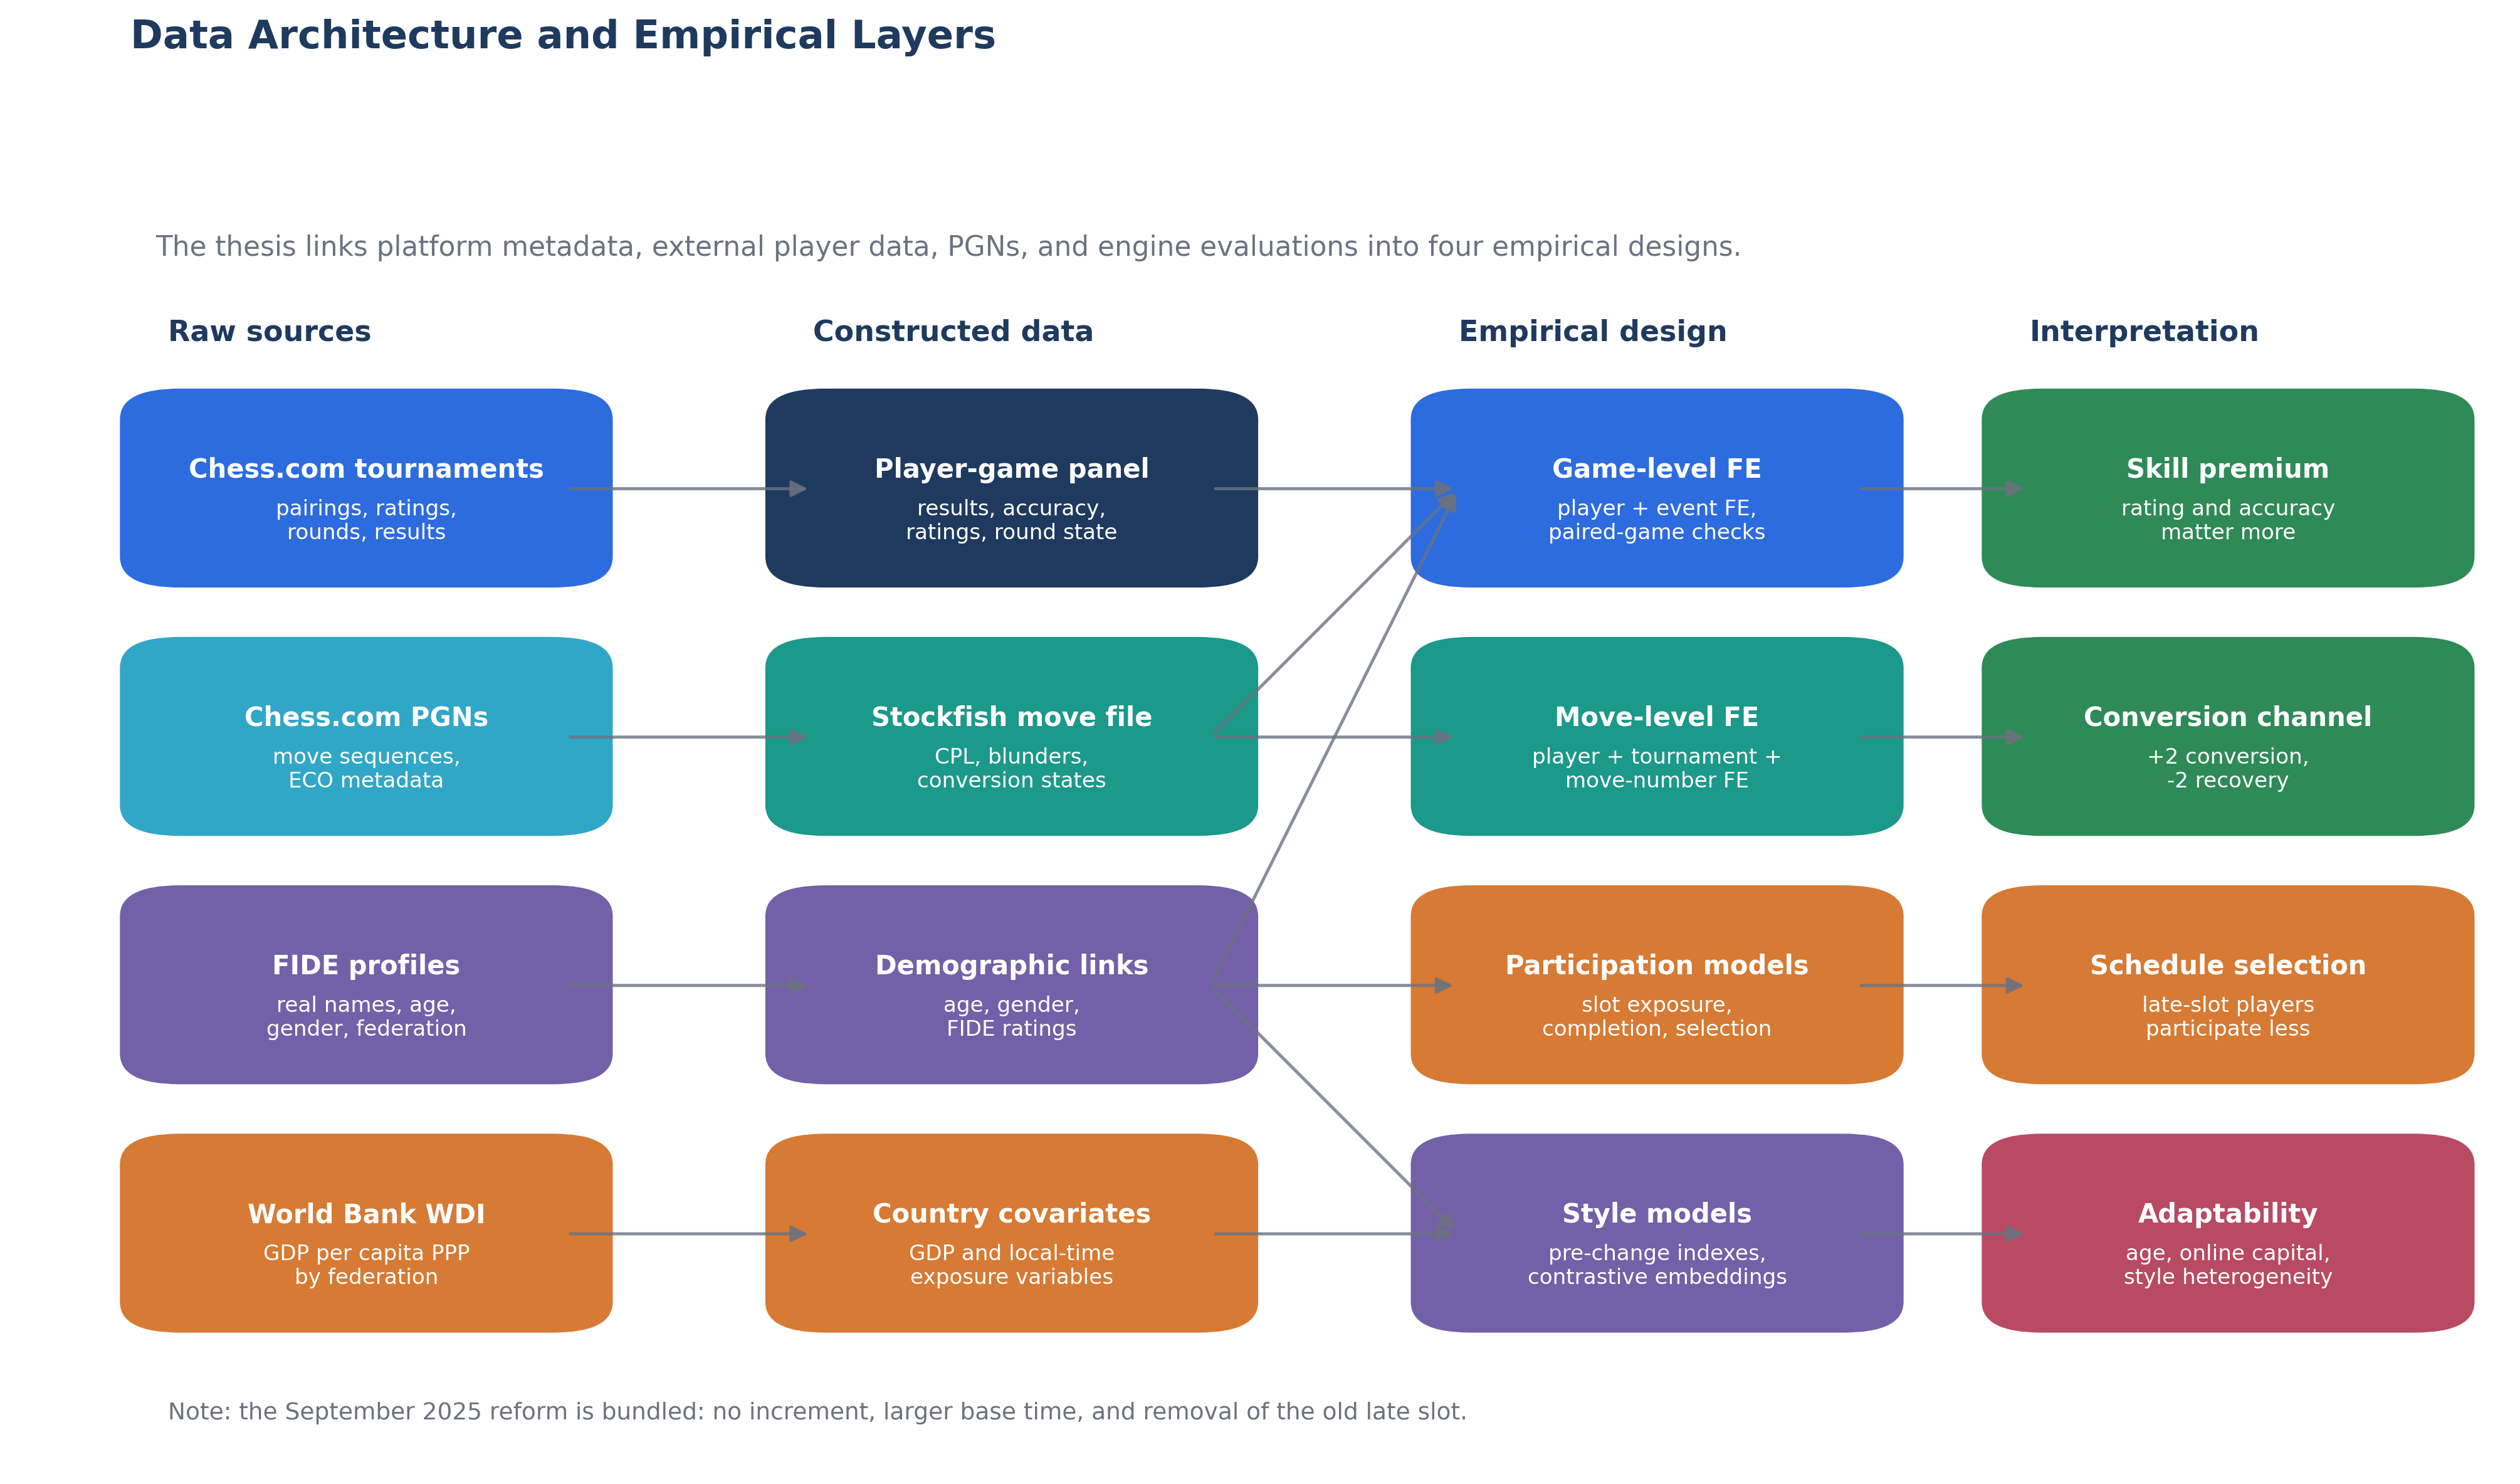
\includegraphics[width=\textwidth]{figures/figure7_data_design_map.png}
\caption{Data architecture and empirical layers used in the thesis.}
\label{fig:data-design-map}
\end{figure}

\subsection{Accuracy Variable Creation}

This variable is one of the key factors in our analysis. Chess.com accuracy is a game-level move-quality metric on a 0 to 100 scale. It is not identical to centipawn loss and Chess.com does not fully publish the exact proprietary formula, but it is widely understood by players and is available directly on many analyzed games. It is useful for the player-game production-function analysis because it provides a high-level measure of how well each player played in the game.

The main difficulty is missing data. Chess.com accuracy is available only after a game has been analyzed on Chess.com platform by someone. Strong or famous players are more likely to have games analyzed by viewers, stream audiences, or the players themselves. This creates a potential selection bias if analyzed games are systematically different from non-analyzed games. To reduce this problem, the project used an automated browser workflow to open game pages, trigger Chess.com's accuracy calculation where needed, wait for the analysis to complete, and then scrape the resulting accuracy. Because Chess.com pages are protected by anti-bot and Cloudflare systems, the collection process required robust browser automation, proxies, and CAPTCHA handling. The final accuracy dataset is therefore much closer to tournament coverage than the initially available analyzed-game subset.

Table \ref{tab:accuracy-summary} reports simple descriptive statistics for the accuracy variables in the main game metadata. White's mean accuracy is slightly higher than Black's, but the difference is small relative to the within-player and within-game variation used in the regressions.

\begin{table}[H]
\centering
\caption{Accuracy Summary by Color}
\label{tab:accuracy-summary}
\begin{tabular}{lrrrrr}
\toprule
Variable & Mean & Std. dev. & Min & Median & Max \\
\midrule
Accuracy White & 83.62 & 7.55 & 0.00 & 84.00 & 100.00 \\
Accuracy Black & 82.86 & 7.83 & 0.00 & 83.20 & 100.00 \\
\bottomrule
\end{tabular}
\end{table}

Table \ref{tab:metadata-summary} summarizes the main raw game-level variables before the most restrictive regression filters. Mean Chess.com ratings are around 2570 for both colors, which confirms that the sample consists of elite titled players. The mean White result is slightly above 0.5, consistent with the usual first-move advantage in chess. The analysis below does not rely on raw color comparisons because the main regressions control for color and include player and event fixed effects.

\begin{table}[H]
\centering
\caption{Selected Descriptive Statistics}
\label{tab:metadata-summary}
\begin{adjustbox}{max width=\textwidth}
\begin{tabular}{lrrrrrr}
\toprule
Variable & Mean & Std. dev. & Std. error & Min & Median & Max \\
\midrule
Rating White & 2576.49 & 285.67 & 0.42 & 0 & 2573 & 3319 \\
Rating Black & 2572.43 & 286.79 & 0.42 & 0 & 2568 & 3319 \\
Result White & 0.53 & 0.48 & 0.00 & 0 & 0.50 & 1 \\
Result Black & 0.47 & 0.48 & 0.00 & 0 & 0.50 & 1 \\
Accuracy White & 83.62 & 7.55 & 0.01 & 0 & 84.00 & 100 \\
Accuracy Black & 82.86 & 7.83 & 0.01 & 0 & 83.20 & 100 \\
\bottomrule
\end{tabular}
\end{adjustbox}
\end{table}

\subsection{Data Cleaning Rules}

Several cleaning rules are applied before the data science analysis. First, games with missing core identifiers, missing player names, missing event identifiers, or invalid results are removed (there are only $\approx100$ of them due to random access problems). Second, the analysis excludes observations from banned or anonymous accounts when these accounts cannot be linked to stable player identities. Third, games involving non-titled or improperly identified accounts are removed from specifications that require the titled-player population. Fourth, observations with impossible or placeholder ratings are dropped in specifications where rating differences are the key treatment interaction. Fifth, FIDE-based demographic and country variables are used only when the username-to-real-name match is sufficiently reliable. Ambiguous or unmatched cases are left missing for those specifications rather than forced into noisy demographic cells.

Accuracy-based models use additional restrictions. Games with accuracy equal to exactly 0 or exactly 100 are excluded from the main accuracy regressions. These values are often generated by missing analysis, parsing failures, very short games, or edge cases in Chess.com's accuracy display. Keeping them would mechanically create extreme values that are not comparable to normal analyzed games. The main accuracy models also exclude round 1 in some specifications, because first-round Swiss pairings can be unusually uneven and may mix the rule-change effect with mechanical pairing differences.

Move-level data require another layer of cleaning. PGNs must be parsable, moves must be legal from the reconstructed board state, and Stockfish evaluations must be available from the relevant player's perspective. Mate scores and extreme engine evaluations can produce very large centipawn losses. The main move-level regressions therefore use capped centipawn loss, \texttt{cp\_loss\_cap}, capped at 1000 centipawns. This preserves information about large mistakes while preventing a small number of mate-score positions from dominating linear models.

\subsection{PGN and Stockfish Data}

The move-level analysis uses PGNs scraped from Chess.com game links. The PGNs provide the sequence of moves, player names, game result, event information, opening metadata where available, clock annotations, and board states that can be reconstructed using a chess parser. For each move with a clock annotation, the pipeline records the player's clock after the move. The clock before the move is recovered from the previous own clock state, taking the time-control increment into account for 3+1 games. The difference gives \texttt{time\_spent}. The resulting variables include \texttt{time\_before\_move}, \texttt{time\_after\_move}, \texttt{time\_spent}, low-clock indicators at 5, 10, and 30 seconds, first entry into low-clock states, final clock, and clock reserves at moves 10, 20, and 30.

Stockfish was used to evaluate positions and moves. For each legal move in a parsed game, the script reconstructs the pre-move board, evaluates the position before and after the move from the mover's perspective, and computes centipawn loss. A move with a large loss relative to the engine benchmark is classified as an inaccuracy, mistake, or blunder using transparent thresholds: 50, 100, and 200 centipawns. The engine analysis was run in two scraping waves because the Chess.com PGN collection was built over time. 

The combined Stockfish mechanism sample used in the current thesis contains 70,868,483 centipawn rows read, 27,517,197 usable move rows after joining to metadata and applying filters, 319,095 games, 616,731 player-games, 5,768 players, and 148 tournaments. The broader clock-feature panel, which is used for the clock-specific mechanism tests, contains 1,556,230 matched player-games, 794,684 games, 7,947 players, 406 event time slots, and about 69.0 million weighted move observations. The gap between rows read and usable rows mostly comes from metadata matching and the fact that not all scraped PGN games are in the cleaned regression metadata.

\subsection{Variables Created on Move-Level}

The move-level variables capture both board-state mechanisms and clock-state mechanisms. Game phase is measured by fullmove number: opening moves 1--10, early middlegame moves 11--20, late middlegame moves 21--35, and endgame moves 36 and later. The variable \texttt{last\_10\_ply} marks the final ten individual moves of the game. These variables describe where in the game errors occur, while the recovered clock variables directly measure remaining-time states.

Critical positions are measured using engine evaluation. The main proxy, called critical equal in the code, equals one when the absolute pre-move engine evaluation from the mover's perspective is below 100 centipawns. This captures positions close to equality, where one mistake can shift the game. Conversion variables are defined at the player-game level. A player reaches a winning position if the engine evaluation reaches at least +200 centipawns from that player's perspective at least ten plies before the game ends. Conversion equals one if the player eventually wins. Similarly, a player reaches a losing position if the evaluation falls below -200 centipawns, and defensive escape equals one if the player eventually draws or wins.

Clock variables are constructed at both move and player-game levels. At the move level, the analysis uses clock bins \((>120, 60\text{--}120, 30\text{--}60, 10\text{--}30, 5\text{--}10, 0\text{--}5\) seconds), time spent on the move, whether the player starts or ends the move below 5, 10, or 30 seconds, and event-time indicators around the first crossing below a low-clock threshold. At the player-game level, the analysis aggregates these measures into low-clock exposure shares, mean time spent, final clock, move-10 clock reserve, low-clock centipawn loss, low-clock blunder rates, conversion while personally low on time, and conversion or escape when the opponent is low on time.

Additional PGN-derived features measure opening, complexity, simplification, and style. Opening depth is parsed from Chess.com's ECO and opening URL information. Complexity measures include legal-move counts, high-legal-move shares, pieces remaining, material remaining, and engine-evaluation volatility. Simplification variables include captures by move 20, queen-off indicators by moves 20 and 30, pieces remaining by move 30, material remaining by move 30, and a simplified-position indicator. These variables are mainly used to test mechanisms that later turn out to be weak or null.

\subsection{Style Features and Neural Data}

The style analysis uses only pre-change games to avoid post-treatment bias. Interpretable player-level style features are constructed from moves and Stockfish evaluations. The main indexes are:

\begin{itemize}
    \item \texttt{clean\_style\_index}: high no-blunder-game rate and low own error rates;
    \item \texttt{chaos\_creator\_index}: high eval-swing, captures, checks, decisive games, and opponent errors after the player's moves;
    \item \texttt{self\_risk\_index}: high own blunders, own mistakes, high upper-tail centipawn loss, and volatile own move quality;
    \item \texttt{practical\_chaos\_index}: chaos creation net of self-risk.
\end{itemize}

All component variables are winsorized at the 1st and 99th percentiles, standardized across players, averaged within each index, and then standardized again. The key advantage of this design is that style variables are predetermined relative to the reform.

For the neural style analysis, the same pre-change move data are converted into player-game move sequences after removing opening theory and the final moves of long games. The model specification, cluster construction, and cluster results are described together with the style findings in Section \ref{sec:playing-style}.

\section{Empirical Strategy}

\subsection{Treatment Definition and Interpretation}

The treatment is the post-reform Titled Tuesday environment. Let \(\text{Post}_t\) be an indicator equal to one for events played on or after September 2, 2025 and zero for events before that date. In the code and result tables this variable is denoted \texttt{format\_5\_0}. It captures the combined institutional change from 3+1 with two weekly time slots to 5+0 with one weekly time slot.

The treatment is not randomized. The empirical strategy therefore relies on within-player comparisons, event fixed effects, observable game controls, and robustness tests. The interpretation is strongest when estimates are stable across player fixed effects, event fixed effects, paired-game fixed effects, near-window samples, balanced-player samples, and placebo cutoffs. The interpretation is more cautious when placebo cutoffs or event studies show pre-existing trends.

\begin{table}[H]
\centering
\caption{Empirical Designs and Interpretation of Key Coefficients}
\label{tab:empirical-design-catalog}
\small
\begin{adjustbox}{max width=\textwidth}
\begin{tabular}{p{0.19\textwidth} p{0.24\textwidth} p{0.25\textwidth} p{0.25\textwidth}}
\toprule
Design layer & Estimand & Main controls and fixed effects & Interpretation \\
\midrule
Player-game treatment heterogeneity & \(\text{Post} \times X_{igt}\) in result or accuracy models & Player FE, event FE, ratings, color, round FE; clustered by player and event & Whether a player trait or game circumstance became more valuable after the switch to 5+0 \\
Paired-game fixed effects & \(\text{Post} \times X_{igt}\) with game FE & Player FE and game FE; comparison across the two sides of the same game & Robustness check absorbing all game-level shocks shared by both players \\
Accuracy production function & \(\text{Post} \times \text{AccuracyDiff10}_{igt}\) & Player FE, event FE or game FE, round/color/rating controls & Whether realized move-quality advantages converted more strongly into points under 5+0 \\
Time-slot displacement & \(\text{Post} \times \text{PreLateShare}_{i}\) or late-regular indicators & Player FE and event FE for games/events; player-level controls for participation & Whether removal of the late slot affected participation, completion, score, and rank \\
Move-level Stockfish mechanisms & \(\text{Post} \times M_{igmt}\) and triple interactions & Player FE, tournament FE, move-number FE; clustered by player and tournament & Whether late, final, critical, or complex positions became more costly after the reform \\
Clock-time mechanisms & \(\text{Post} \times C_{igmt}\), clock-bin interactions, and first-low-clock event studies & Player FE, event FE, move-number FE or player-game aggregations; clustered by player & Whether severe time trouble, increment removal, and opponent clock weakness changed move quality and conversion under 5+0 \\
Conversion and recovery & \(\text{Post} \times \text{RatingDiff100}_{igt}\) after reaching +2 or -2 & Player-game outcomes with player and tournament controls & Whether stronger players managed winning and losing positions more effectively under 5+0 \\
Pre-change style traits & \(\text{Post} \times S_i^{pre}\) & Player FE, event FE, rating/color/round controls & Whether predetermined playing styles or skills became more or less rewarded after the reform \\
\bottomrule
\end{tabular}
\end{adjustbox}
\end{table}


\subsection{Baseline Player-Game Difference-in-Differences}

The main player-game outcome is \(\text{Result}_{iget}\), the score result of player \(i\) in game \(g\) during event \(t\). It equals one for a win, one half for a draw, and zero for a loss. The baseline specification is:

\begin{equation}
\label{eq:baseline}
Y_{iget}
= \beta \left(\text{Post}_{t} \times X_{iget}\right)
+ \theta X_{iget}
+ \Gamma' W_{iget}
+ \alpha_i
+ \delta_t
+ \varepsilon_{iget}.
\end{equation}

\noindent Here \(Y_{iget}\) is the outcome, \(X_{iget}\) is the mechanism or player characteristic of interest, \(W_{iget}\) includes controls, \(\alpha_i\) are player fixed effects, and \(\delta_t\) are event fixed effects. The standard control set includes the player's rating, the opponent's rating, a White-piece indicator, and round fixed effects. Standard errors are clustered by player and event.

The key coefficient is \(\beta\). For example, when \(X_{iget}\) is \(\text{rating\_diff100}_{iget}\), \(\beta\) measures how much more valuable a 100-point rating advantage became after the switch to 5+0. Because player fixed effects absorb time-invariant player strength and style, identification comes from changes in the value of within-player game circumstances after the rule change.

Several variants of Equation \eqref{eq:baseline} are used:

\begin{itemize}
    \item event fixed effects with all rounds after round 1;
    \item exclusion of rounds 1 and 2;
    \item a near-window sample around the reform;
    \item balanced-player samples containing players observed before and after the reform;
    \item paired-game fixed effects using \(\alpha_i\) and game fixed effects, so the comparison is within the same game across the two players;
    \item placebo cutoffs before September 2025;
    \item event-study specifications by month relative to the reform.
\end{itemize}

The paired-game fixed-effect version is:

\begin{equation}
\label{eq:gamefe}
Y_{iget}
= \beta \left(\text{Post}_{t} \times X_{iget}\right)
+ \Gamma' W_{iget}
+ \alpha_i
+ \lambda_g
+ \varepsilon_{iget},
\end{equation}

\noindent where \(\lambda_g\) is a game fixed effect. This specification compares the two sides of the same game after absorbing game-level conditions common to both players.

\subsection{Accuracy-to-Outcome Production Function}

Let's proceed to an example of this regression specification in use. Accuracy is an in-game performance measure, not a predetermined characteristic. For this reason the accuracy specification is interpreted as a production-function test rather than a causal treatment effect of accuracy. The central question is whether the same measured accuracy advantage translated into more points under 5+0:

\begin{equation}
\label{eq:accuracy}
\text{Result}_{iget}
= \beta \left(\text{Post}_{t} \times \text{AccuracyDiff10}_{iget}\right)
+ \theta \text{AccuracyDiff10}_{iget}
+ \Gamma' W_{iget}
+ \alpha_i
+ \delta_t
+ \varepsilon_{iget}.
\end{equation}

\noindent \(\text{AccuracyDiff10}\) is the player's accuracy minus the opponent's accuracy, divided by 10. A positive \(\beta\) means that points became more tightly linked to observed move-quality advantages after the reform. This model is estimated with event fixed effects, paired-game fixed effects, round restrictions, placebo cutoffs, and event studies.

Additional production-function models test whether rating favorites or online specialists convert a given accuracy edge more efficiently:

\begin{equation}
\label{eq:tripleaccuracy}
\begin{aligned}
\text{Result}_{iget}
= {} & \beta_1(\text{Post}_t \times \text{AccuracyDiff10}_{iget}) \\
& + \beta_2(\text{Post}_t \times \text{AccuracyDiff10}_{iget} \times Z_{iget}) \\
& + \Gamma' W_{iget} + \alpha_i + \delta_t + \varepsilon_{iget}.
\end{aligned}
\end{equation}

\noindent where \(Z_{iget}\) is rating advantage, online-capital advantage, or tournament-state status. The evidence below shows that accuracy conversion increased overall, but not mainly because the same accuracy edge became more valuable only for favorites or online specialists.

\subsection{Time-Slot Displacement}

The schedule component of the reform is analyzed separately. Pre-change events are classified as early or late based on event hour. For each player, \(\text{PreLateShare}_i\) is the share of pre-change events played in the late slot. A binary \(\text{LateRegular}_i\) indicator equals one for players with at least four pre-change events, at least three late events, and a late-share of at least 0.60.

The game-level displacement model is:

\begin{equation}
\label{eq:timeslotgame}
Y_{iget}
= \beta(\text{Post}_t \times \text{PreLateShare}_i)
+ \Gamma' W_{iget}
+ \alpha_i
+ \delta_t
+ \varepsilon_{iget}.
\end{equation}

The tournament-level version uses player-event outcomes such as tournament score after round 1, rank percentile, mean accuracy after round 1, games completed, and completion indicators:

\begin{equation}
\label{eq:timeslottournament}
Y_{iet}
= \beta(\text{Post}_t \times \text{PreLateShare}_i)
+ \Gamma' W_{iet}
+ \alpha_i
+ \delta_t
+ \varepsilon_{iet}.
\end{equation}

Finally, selection into post-change participation is estimated at the player level:

\begin{equation}
\label{eq:participation}
\text{PostParticipation}_{i}
= \beta \text{PreLateShare}_{i}
+ \Gamma' Z_i
+ u_i,
\end{equation}

\noindent where \(Z_i\) includes pre-change event count, pre-change rating, and title controls. This model asks whether late-slot exposure predicts appearing in the post-change era at all.

\subsection{Move-Level Stockfish Models}

Move-level outcomes include capped centipawn loss, blunder indicators, mistake indicators, and inaccuracy indicators. Let \(m\) index a move by player \(i\) in game \(g\), tournament \(t\), and fullmove number \(n\). The baseline move-level mechanism model is:

\begin{equation}
\label{eq:movelevel}
Y_{igmt}
= \beta(\text{Post}_t \times M_{igmt})
+ \theta M_{igmt}
+ \Gamma' W_{igmt}
+ \alpha_i
+ \delta_t
+ \mu_n
+ \varepsilon_{igmt}.
\end{equation}

\noindent \(M_{igmt}\) is a move environment indicator such as late phase, final ten plies, or critical equal position. \(\mu_n\) are fullmove-number fixed effects. Standard errors are clustered by player and tournament. A positive \(\beta\) in the centipawn-loss model means that the relevant move environment became more costly after the reform.

Age and gender heterogeneity are estimated with triple interactions:

\begin{equation}
\label{eq:movetriple}
Y_{igmt}
= \beta_1(\text{Post}_t \times M_{igmt})
+ \beta_2(\text{Post}_t \times H_i)
+ \beta_3(\text{Post}_t \times H_i \times M_{igmt})
+ \Gamma' W_{igmt}
+ \alpha_i
+ \delta_t
+ \mu_n
+ \varepsilon_{igmt},
\end{equation}

\noindent where \(H_i\) is age in ten-year units, female status, GDP, or another player characteristic. The coefficient \(\beta_3\) tests whether the post-change cost of a given move environment differs across player types.

\subsection{Clock-Time Mechanism Models}

Clock-time models use the same reform indicator but replace board-state indicators with direct remaining-time measures. At the player-game level, the main exposure model estimates whether low-clock shares changed after the reform:

\begin{equation}
\label{eq:clockexposure}
\text{LowClockShare}_{igt}
= \beta \text{Post}_t
+ \Gamma' W_{igt}
+ \alpha_i
+ \delta_t
+ \varepsilon_{igt}.
\end{equation}

\noindent At the move level, the panic-threshold specification bins the player's remaining time before the move:

\begin{equation}
\label{eq:clockbins}
Y_{igmt}
= \sum_b \beta_b \mathbf{1}\{\text{ClockBin}_{igmt}=b\}
+ \sum_b \gamma_b \left(\text{Post}_t \times \mathbf{1}\{\text{ClockBin}_{igmt}=b\}\right)
+ \alpha_i+\delta_t+\mu_n+\varepsilon_{igmt}.
\end{equation}

\noindent The omitted bin is more than 120 seconds. The coefficients \(\gamma_b\) measure whether the post-change quality penalty is different in each low-clock region. Additional clock specifications use event time around the first crossing below 30 or 10 seconds, recovery above 10 seconds after first low-clock entry, and player-game conversion outcomes conditional on own or opponent low clock at the first +2 or -2 engine state.

\subsection{Conversion and Defensive Recovery}

Conversion and defensive recovery are estimated at the player-game level. A player is classified as reaching a winning position if the engine evaluation reaches at least +200 centipawns from that player's perspective at least ten plies before the end. The main conversion outcome equals one if the player eventually wins:

\begin{equation}
\label{eq:conversion}
\text{Converted}_{igt}
= \beta(\text{Post}_t \times \text{RatingDiff100}_{igt})
+ \Gamma' W_{igt}
+ \alpha_i
+ \delta_t
+ \varepsilon_{igt}.
\end{equation}

The defensive recovery model is symmetric. A player is classified as reaching a losing position if the evaluation falls to -200 centipawns or worse. The escape outcome equals one if the player eventually draws or wins:

\begin{equation}
\label{eq:escape}
\text{Escaped}_{igt}
= \beta(\text{Post}_t \times \text{RatingDiff100}_{igt})
+ \Gamma' W_{igt}
+ \alpha_i
+ \delta_t
+ \varepsilon_{igt}.
\end{equation}

Additional deep-conversion outcomes include plies to conversion after +2, whether the advantage falls back below equality after +2, centipawn recovery after -2, and defensive recovery probability. These models connect the game-level skill premium to concrete advantage-management behavior.

\subsection{Style and Pre-Change Traits}

The style analysis uses pre-change player traits to avoid post-treatment bias. Let \(S_i^{pre}\) denote a style index computed only from games before September 2025. The main style specification is:

\begin{equation}
\label{eq:style}
\text{Result}_{iget}
= \beta(\text{Post}_t \times S_i^{pre})
+ \Gamma' W_{iget}
+ \alpha_i
+ \delta_t
+ \varepsilon_{iget}.
\end{equation}

Since \(S_i^{pre}\) is time-invariant at the player level, its main effect is absorbed by player fixed effects. The interaction with \(\text{Post}_t\) measures whether a pre-existing style profile became more or less rewarded after the reform. The most important style indexes are clean style, chaos creation, self-risk, and practical chaos. Related pre-change trait models use defensive skill, complexity tolerance, conversion skill, opening specialization, and cascade resilience as predetermined moderators of post-change performance.

\subsection{Inference and Multiple Testing}

Most regressions use two-way clustered standard errors at the player and event level, or player and game level in paired-game specifications. Move-level models use player and tournament clustering. Because the research design tests many mechanisms, the reported result tables include both raw p-values and Benjamini-Hochberg adjusted q-values where appropriate. The thesis emphasizes results that are statistically strong, economically meaningful, and stable across robustness checks. Results that appear only in one exploratory specification or fail false-discovery adjustment are reported in the null and weak-results section rather than treated as main findings.

\section{Results}

This section reports the main results that are proved to be robust by our analysis. The estimates are grouped into player-game effects, tournament participation effects, move-level mechanisms, and style results. Detailed stargazer-generated tables are included in the project folder \texttt{tables/}; compact versions are shown below for readability.

\begin{figure}[H]
\centering
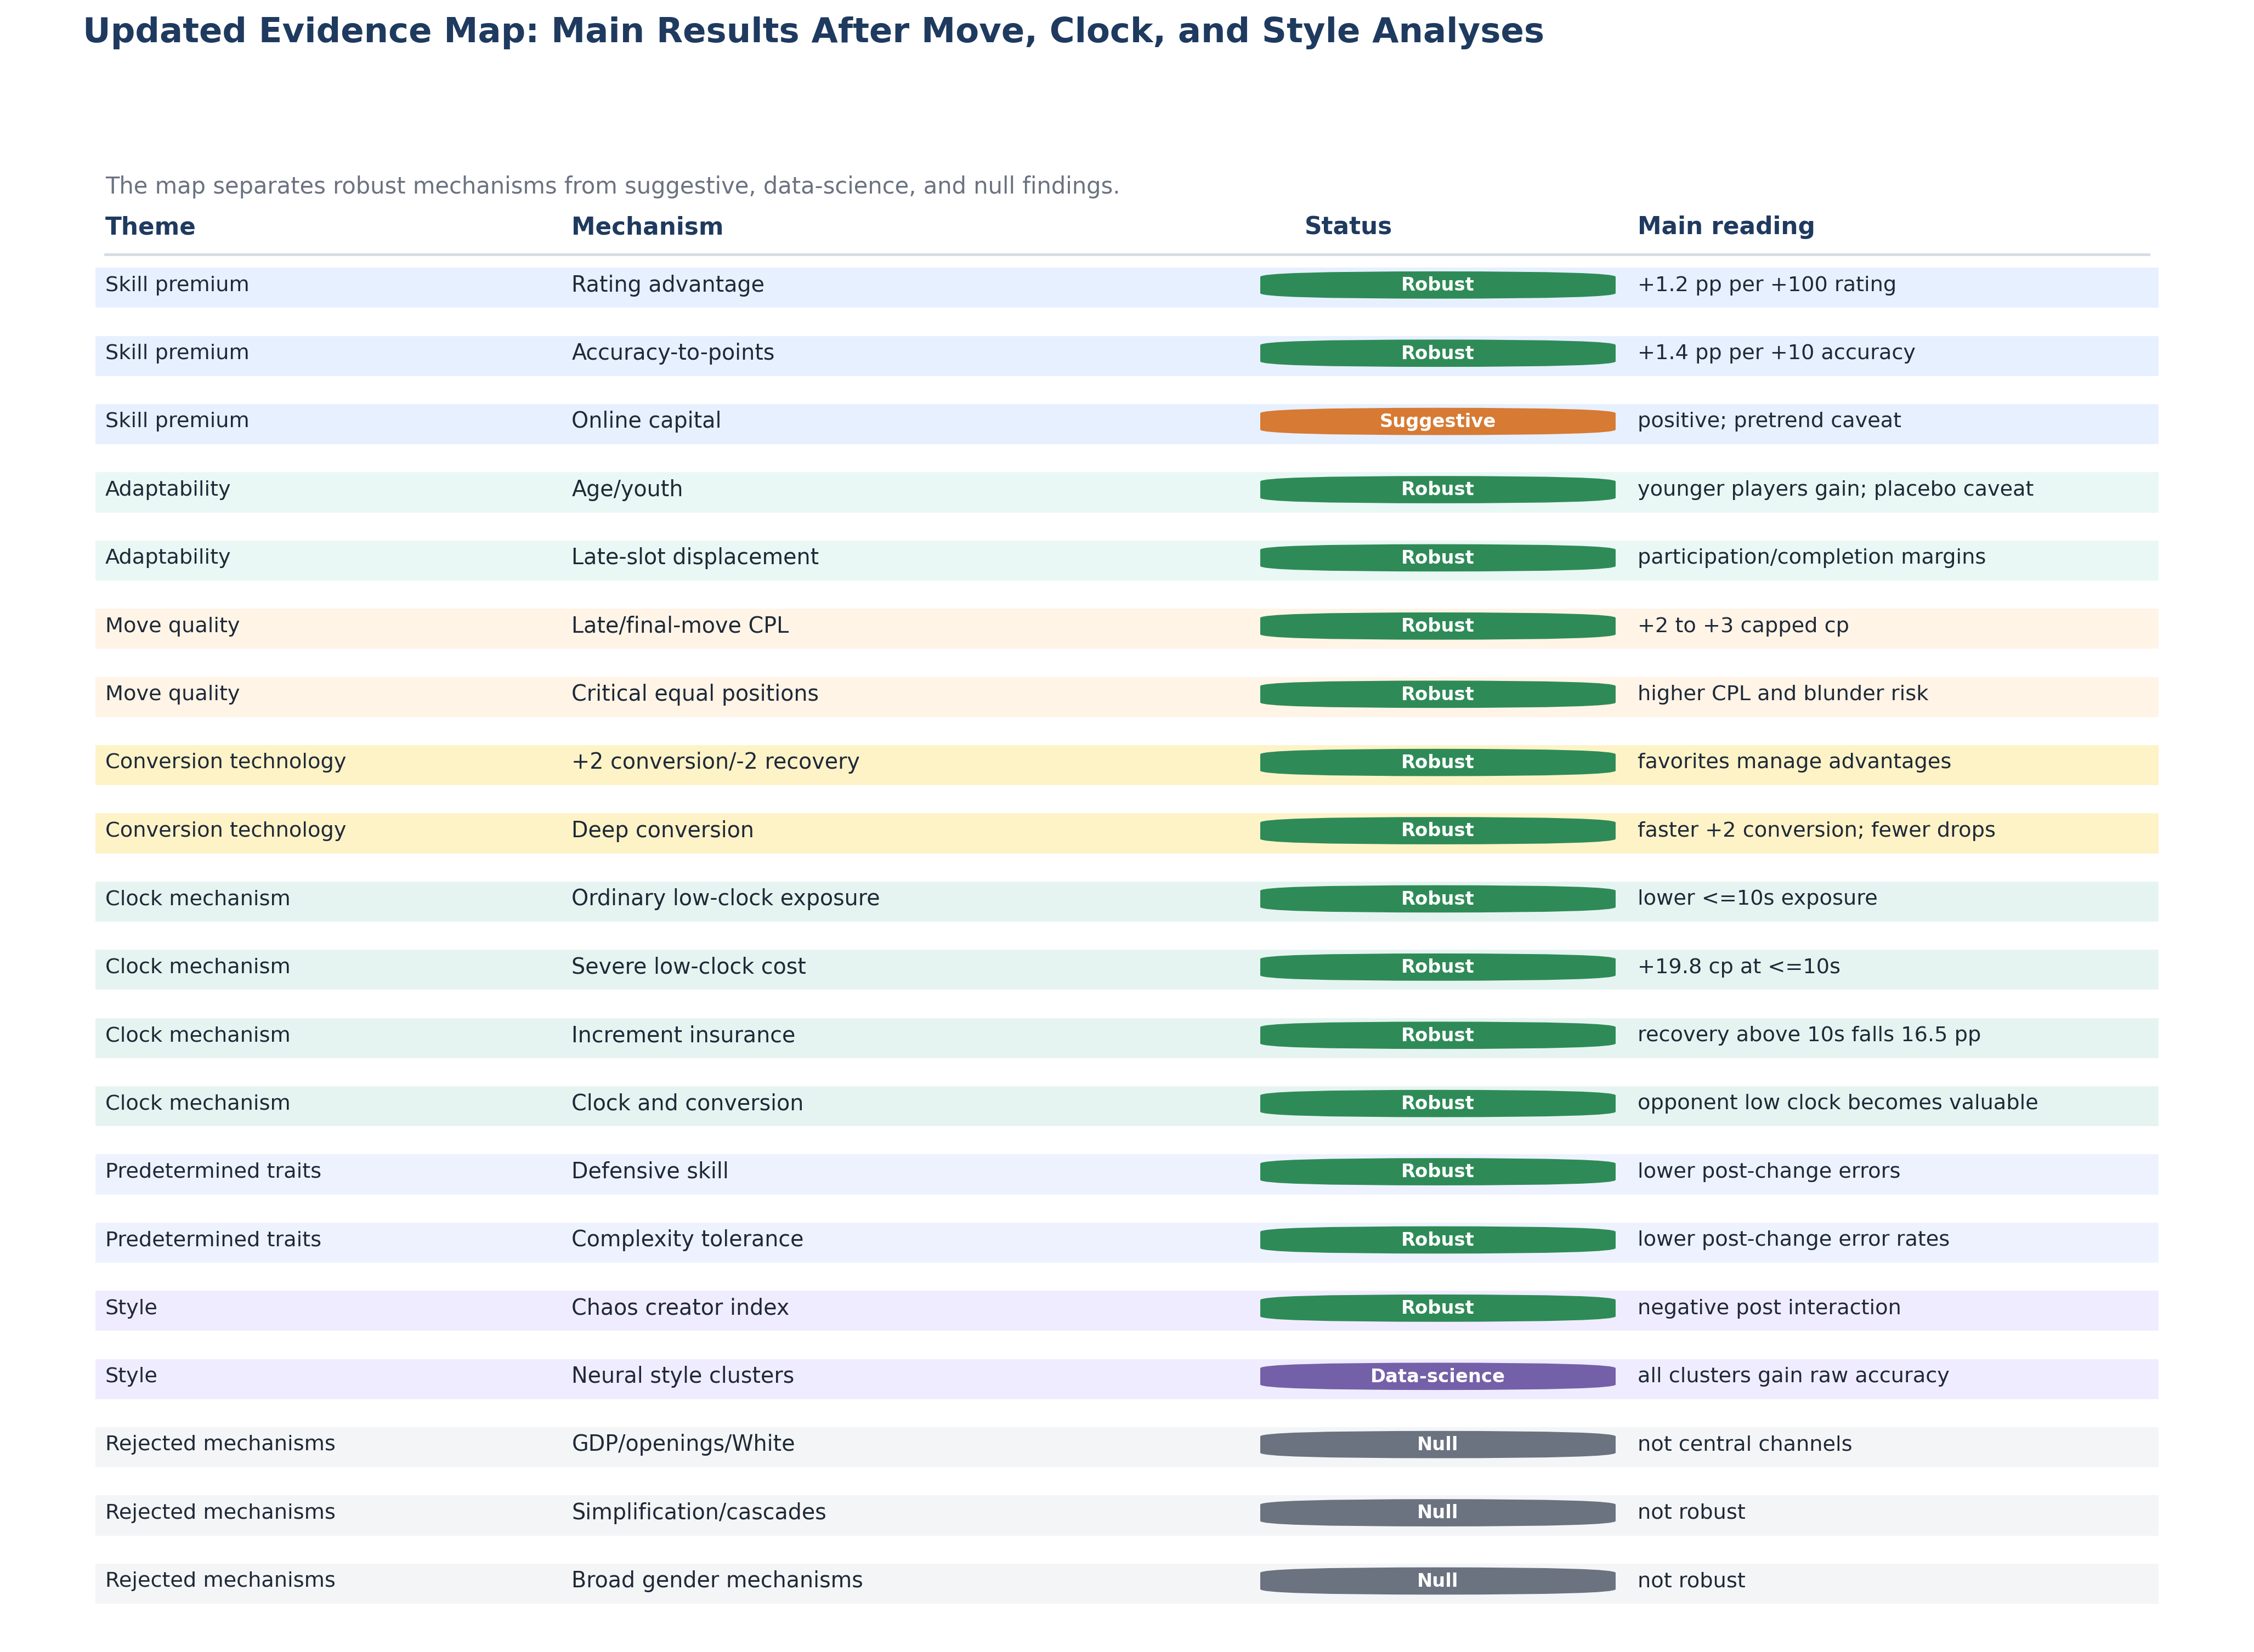
\includegraphics[width=\textwidth]{figures/figure10_clean_outline_evidence_map.png}
\caption{Key findings after the game-level, move-level, clock, and style analyses.}
\label{fig:evidence-map}
\end{figure}

\subsection{Relative Skill Became More Valuable}

The strongest game-level result is that the post-change format increased the return to rating advantage. Table \ref{tab:main-game-results} summarizes the baseline treatment interactions. The coefficient on \(\text{Post} \times \text{RatingDiff100}\) is 0.0119 in the clean thesis table and 0.0122 in the validation report. The interpretation is direct: after the switch to 5+0, a 100-point rating edge was associated with about 1.2 additional percentage points of score result.

\begin{table}[H]
\centering
\caption{Baseline Game-Level Treatment Effects}
\label{tab:main-game-results}
\begin{adjustbox}{max width=\textwidth}
\begin{tabular}{llrrrrl}
\toprule
Result & Outcome & Estimate & SE & p-value & N & Unit \\
\midrule
Relative skill return & Player result & 0.0119 & 0.0010 & \(<0.001\) & 1,335,043 & Per +100 rating advantage \\
Accuracy-to-points conversion & Player result & 0.0141 & 0.0023 & \(<0.001\) & 1,284,771 & Per +10 accuracy points \\
Online-platform capital & Player result & 0.0093 & 0.0013 & \(<0.001\) & 1,315,216 & Per +100 Chess.com-over-classical rating \\
Age heterogeneity & Player result & -0.0145 & 0.0016 & \(<0.001\) & 1,335,043 & Per +10 years of age \\
\bottomrule
\end{tabular}
\end{adjustbox}
\end{table}

The magnitude is economically meaningful. A 200-point favorite gained about 2.4 additional percentage points of expected score after the reform. Moving from the 25th to the 75th percentile of rating difference corresponds to about 5.5 percentage points in score share. Win/loss decomposition shows that the effect is not only a draw-margin change. The probability of winning increases by about 1.3 percentage points per 100 rating points, while the probability of losing falls by about 1.2 percentage points. Draw probability changes little.

Table \ref{tab:rating-robustness} shows the main robustness checks. The coefficient remains positive and close in magnitude when early rounds are excluded, when the sample is restricted to a twelve-month window around the reform, when only balanced players are used, and when paired-game fixed effects are added. The paired-game fixed-effect estimate is smaller, about 0.0095, but it remains economically meaningful.

\begin{table}[H]
\centering
\caption{Robustness of the Rating-Advantage Result}
\label{tab:rating-robustness}
\begin{tabular}{lrrl}
\toprule
Specification & Estimate & SE & Interpretation \\
\midrule
Event FE, rounds \(>1\) & 0.0122 & 0.0010 & Main design \\
Exclude rounds 1 and 2 & 0.0139 & 0.0011 & Similar after removing early Swiss noise \\
\(\pm\)12 month window & 0.0134 & 0.0015 & Similar near the reform \\
Balanced players only & 0.0117 & 0.0011 & Similar among repeat players \\
Paired-game FE & 0.0095 & 0.0012 & Same-game comparison \\
Placebo-grid mean & 0.0017 & -- & Much smaller than actual estimate \\
\bottomrule
\end{tabular}
\end{table}

Figure \ref{fig:rating-robustness-advanced} presents the same robustness pattern graphically. The placebo-grid estimate is close to zero and its confidence interval lies far below the estimates from the main designs.

\begin{figure}[H]
\centering
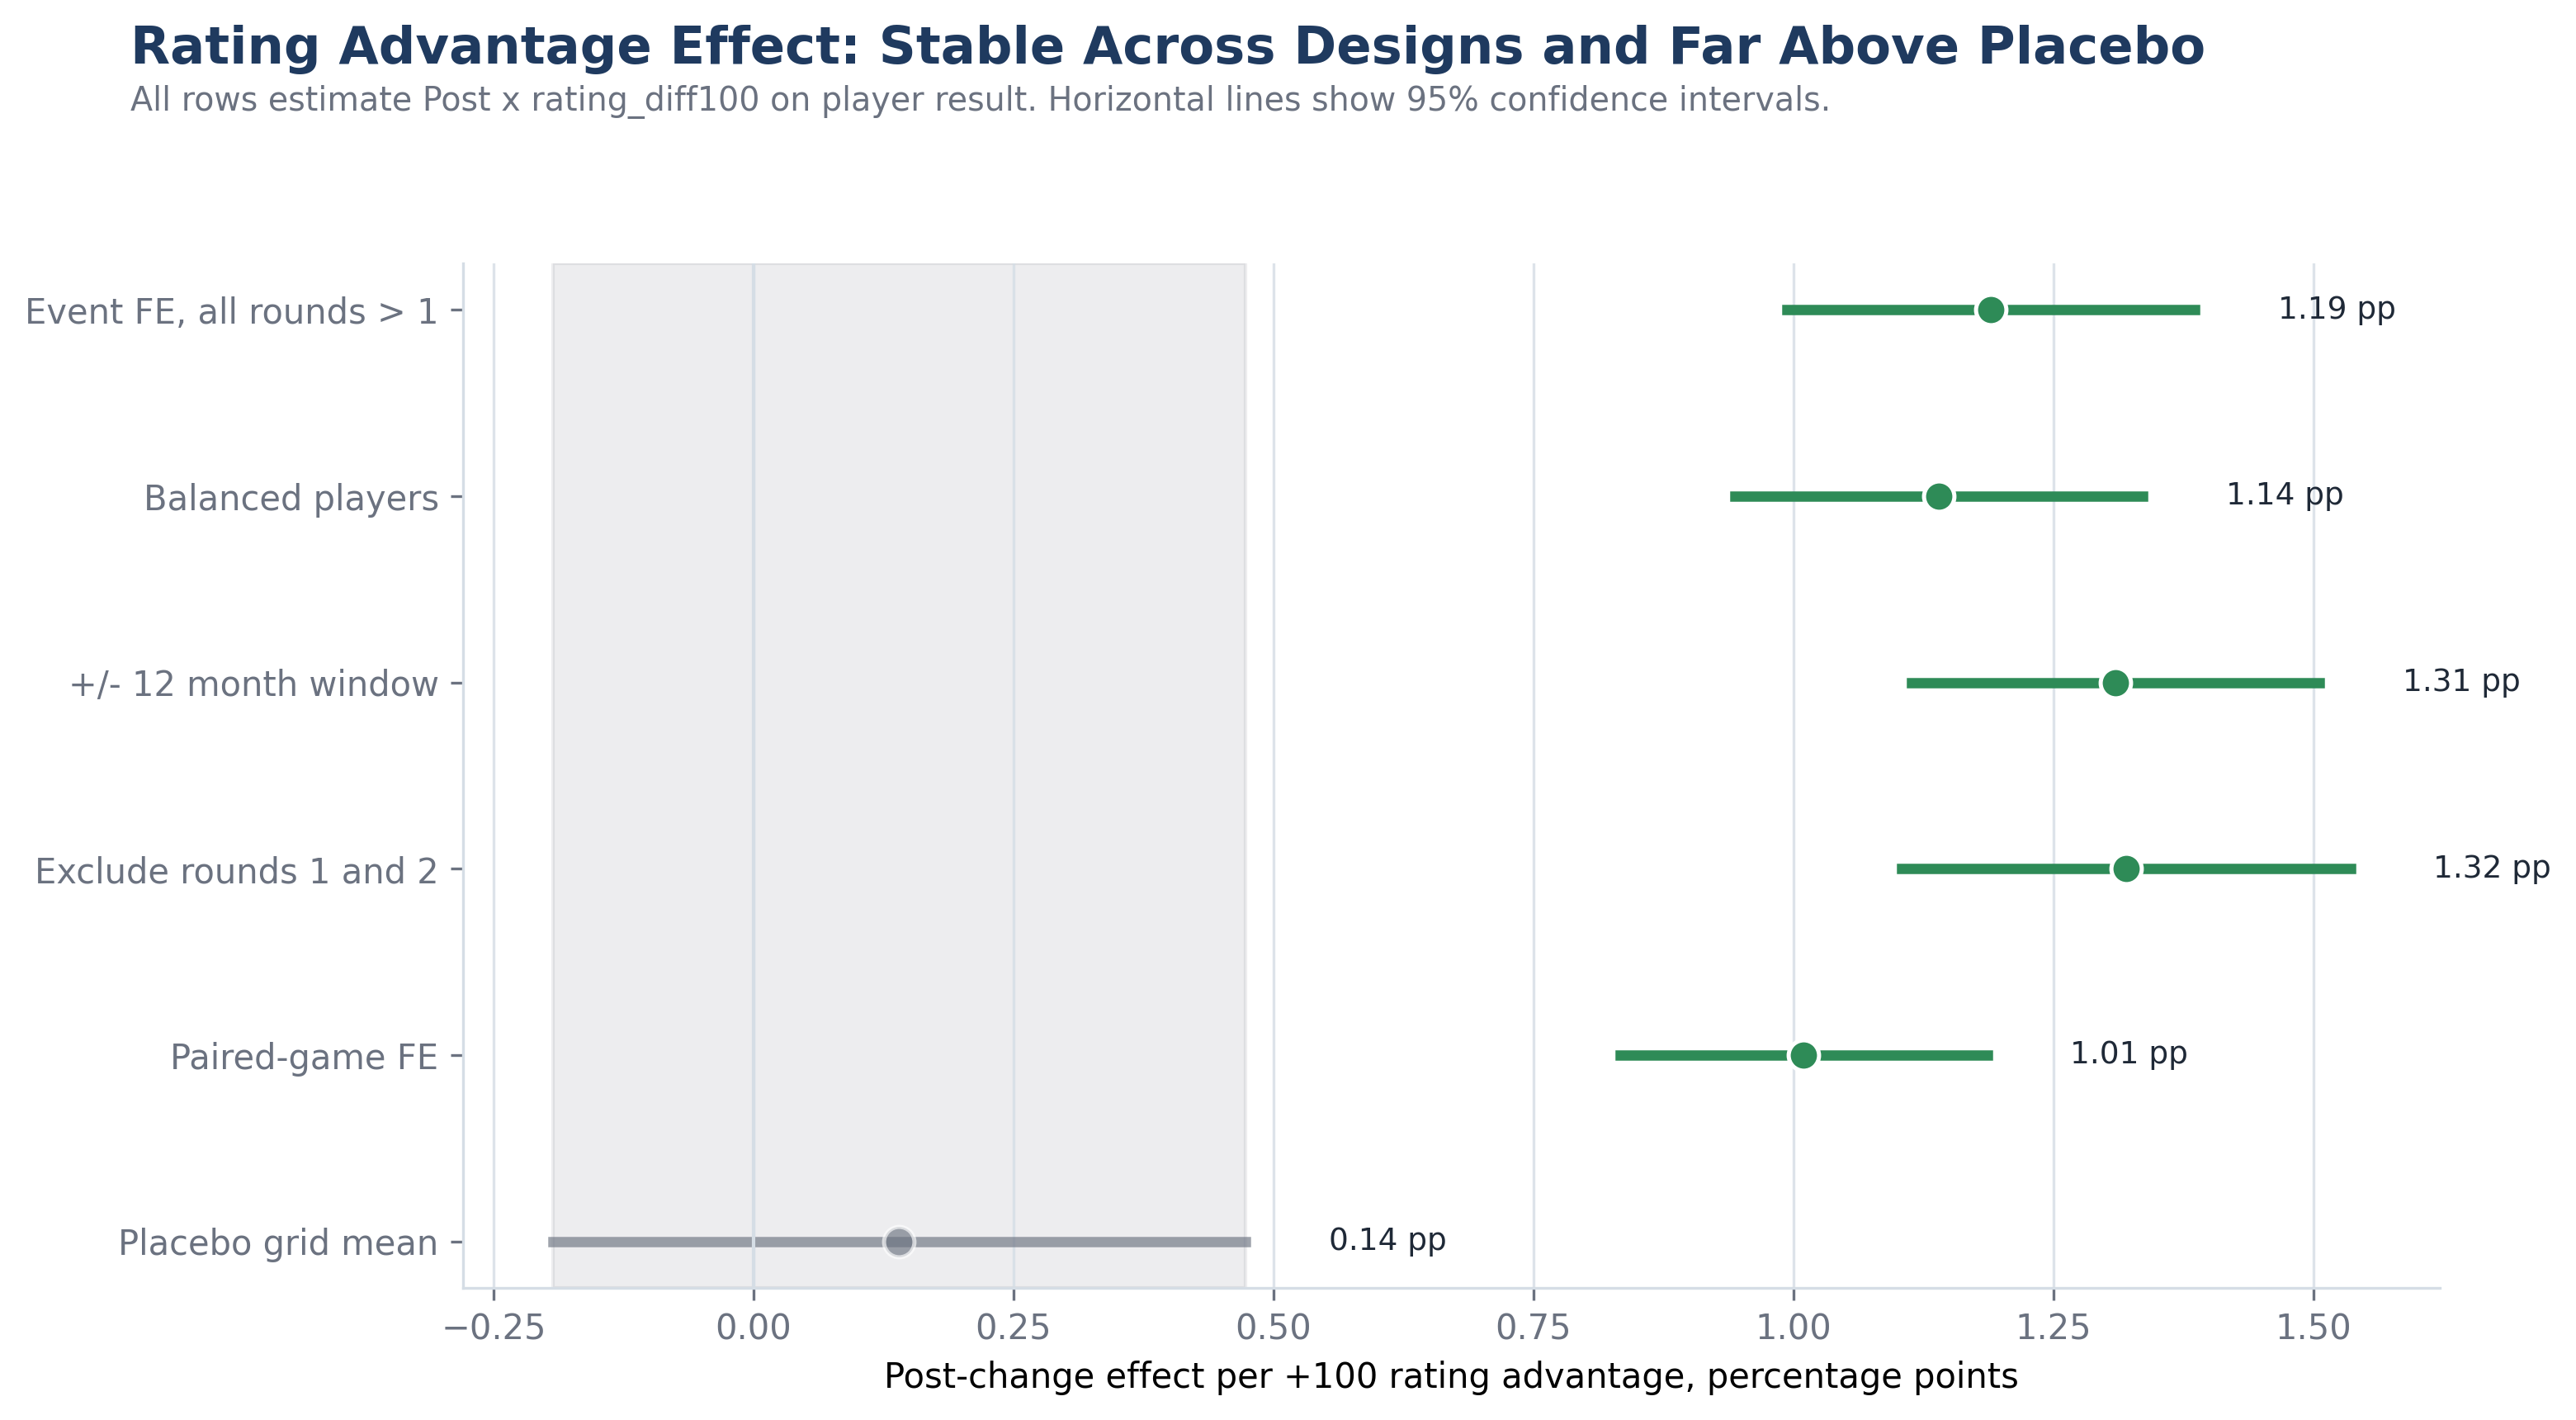
\includegraphics[width=0.92\textwidth]{figures/figure8_rating_robustness_advanced.png}
\caption{Coefficient plot for the rating-advantage result across robustness designs.}
\label{fig:rating-robustness-advanced}
\end{figure}

The placebo evidence is especially important. Across fake pre-reform cutoffs, the mean placebo coefficient is around 0.0017 and the 90th percentile is around 0.0031, far below the actual estimate. The linear pretrend in the pre-period is small and negative, not positive. Figure \ref{fig:rating-event-study} shows the event-study pattern for the rating-difference return and connects it to the newly available clock data. The post-change coefficients rise relative to the pre-change reference period, while the pre-period does not display a comparable upward movement. The clock panels show that ordinary low-clock exposure fell after the reform, but the centipawn-loss penalty of severe low-clock states became much larger under 5+0.

\begin{figure}[H]
\centering
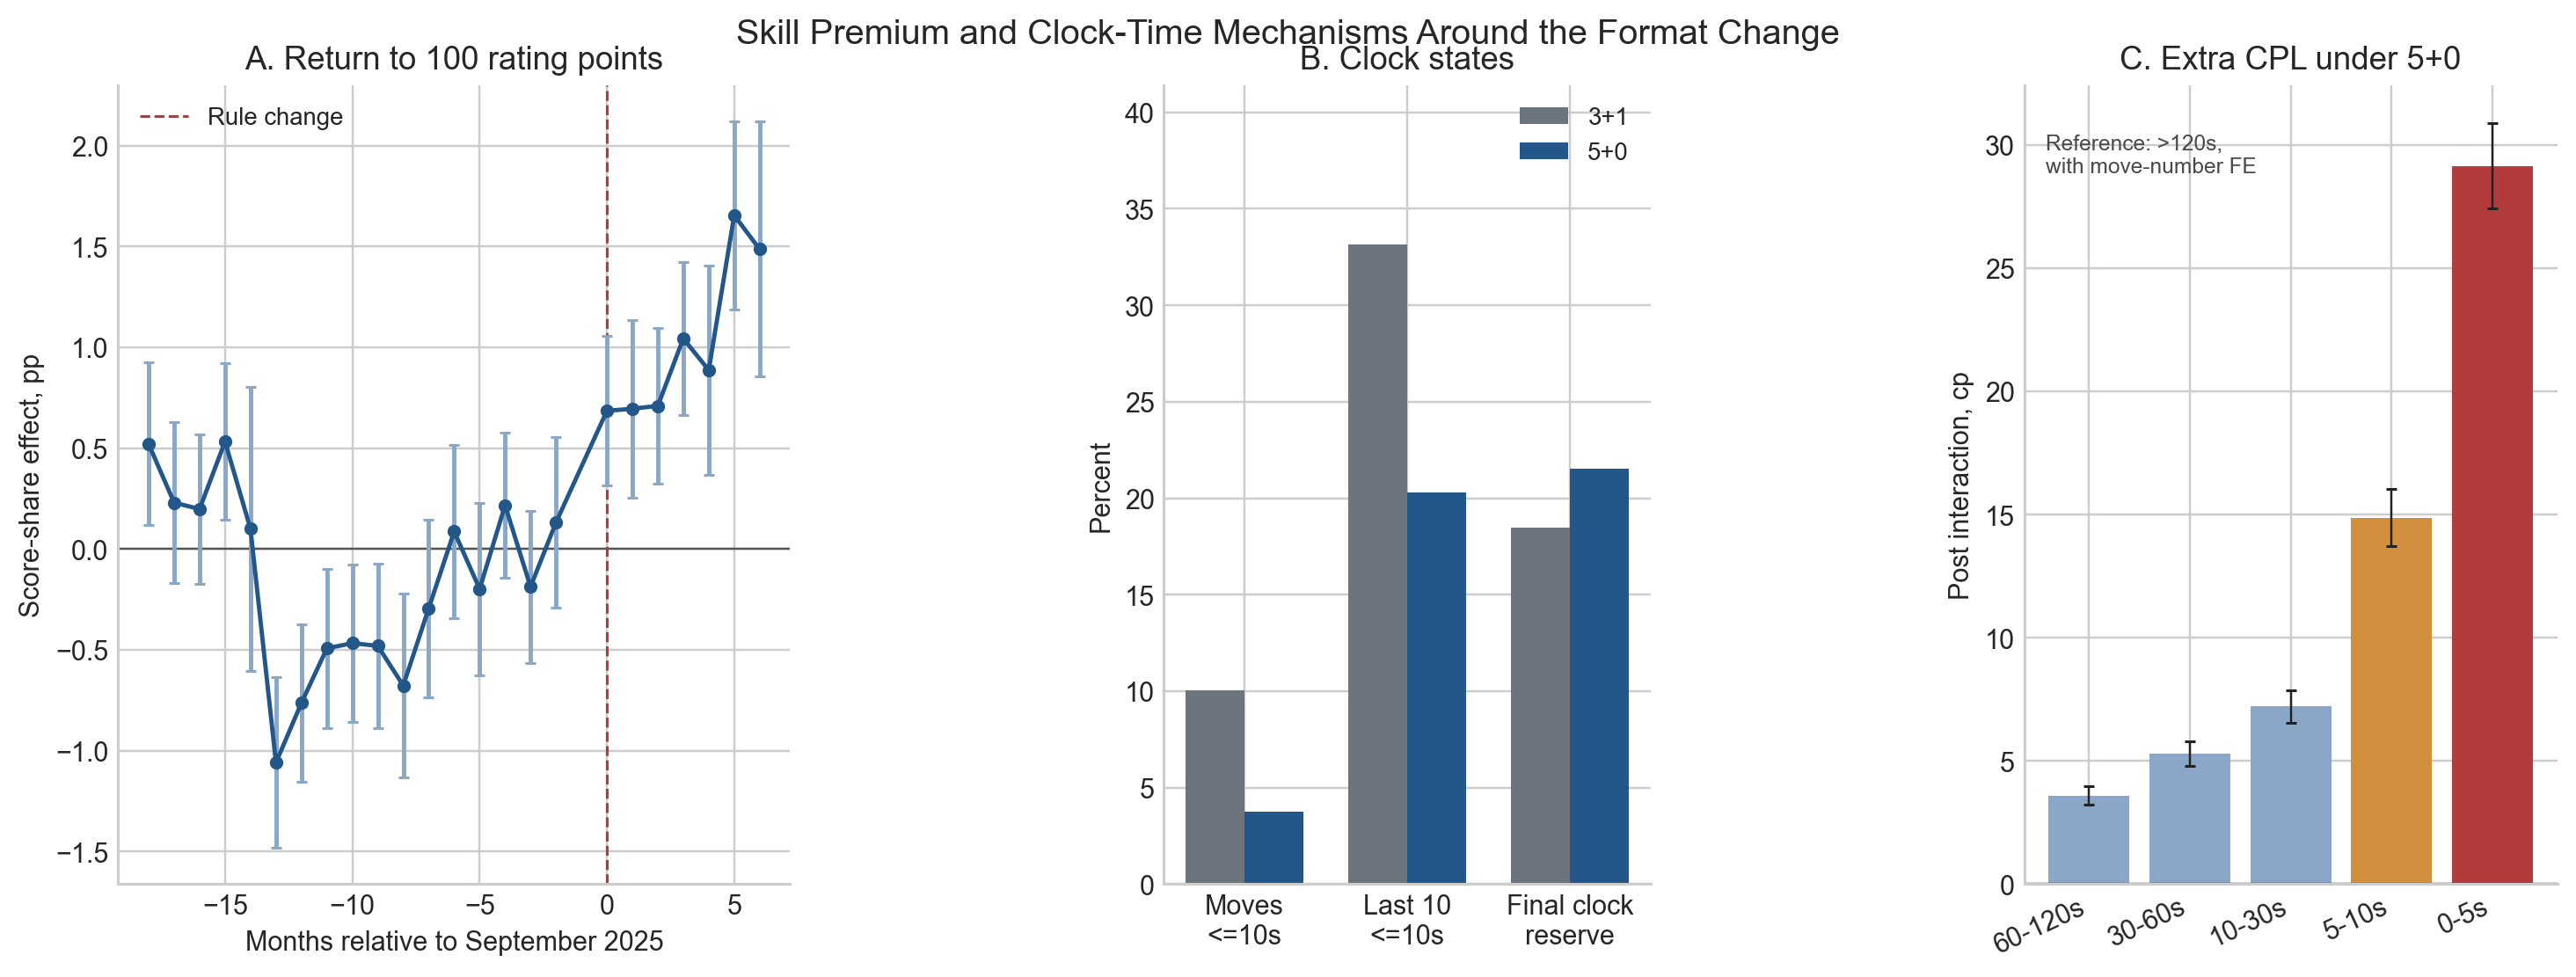
\includegraphics[width=\textwidth]{figures/figure1_rating_diff_event_study.png}
\caption{Rating advantage and clock-time mechanisms around the reform. Panel A reports the event-study return to a 100-point rating advantage. Panel B compares clock exposure and final clock reserve before and after the reform. Panel C reports post-change centipawn-loss interactions by remaining-clock bin, with move-number fixed effects.}
\label{fig:rating-event-study}
\end{figure}

This result is the cleanest evidence in the thesis. It shows that the new format did not primarily increase underdog randomness. Instead, conditional on playing, ex ante stronger players converted their rating advantage more effectively under 5+0.

\subsection{Accuracy Advantages Converted More Strongly into Points}

The production-function result is also strong, though it has a different interpretation. Accuracy is measured inside the game, so it should not be treated as a predetermined causal variable. It is better understood as a measure of the realized quality advantage in the game. The coefficient on \(\text{Post} \times \text{AccuracyDiff10}\) is 0.0141 in the compact thesis table and 0.0347 in the broader production-function battery. Both versions show the same pattern: after the reform, a given accuracy advantage translated into more score share.

In the broader battery, a 10-point accuracy advantage became worth about 3.5 additional percentage points of score share. The effect remains similar with paired-game fixed effects and when rounds 1 and 2 are excluded. The model using result over expected score also remains positive. Placebo estimates are smaller than the actual estimate, although there is evidence of a positive pretrend, so the safest wording is that the reform sharply amplified a pre-existing increase in accuracy-to-result conversion.

The interpretation is that 5+0 made the result more tightly connected to actual move quality. If one player outplayed the opponent by the same amount, that edge was more likely to become a full point or half-point advantage after the rule change. This complements the rating result: stronger players gained, and the mapping from realized quality to points became steeper.

Additional tests show that this production-function shift is not mainly a rating-favorite channel. The triple interaction \(\text{Post} \times \text{AccuracyDiff10} \times \text{RatingDiff100}\) is not statistically clear. The same is true for the online-capital triple interaction. Favorites gained, but not because the same accuracy edge became disproportionately more valuable only for favorites.

\subsection{Online-Platform Capital and Age Adaptability}

The online-platform result suggests that Chess.com-specific skill mattered more after the reform. Players whose Chess.com rating was high relative to classical rating gained about 0.9 to 1.1 percentage points per 100 rating points of online-over-classical advantage. The same broad pattern appears for Chess.com-over-FIDE blitz gaps. This is consistent with the idea that 5+0 online play rewards platform-specific human capital: mouse speed, interface fluency, premoves, practical no-increment experience, and comfort with the Chess.com playing environment.

This result is robust as an association, but it is not as clean as the rating-advantage result. Placebo and event-study checks suggest that returns to online specialization were already rising before September 2025. The most careful interpretation is therefore that the rule change reinforced an ongoing rise in the value of online-specific capital, rather than creating the whole effect from zero.

Age heterogeneity is statistically strong. The main player-game estimate is about -0.0145 per 10 years of age. Within-game age-gap comparisons are also negative: after the reform, older players performed worse relative to younger opponents in the same game. In games between young and old players, the post-change score shifted by about 2.3 percentage points toward the young player. The accuracy result is directionally similar, with older players losing about 0.15 accuracy points per additional decade.

\begin{figure}[H]
\centering
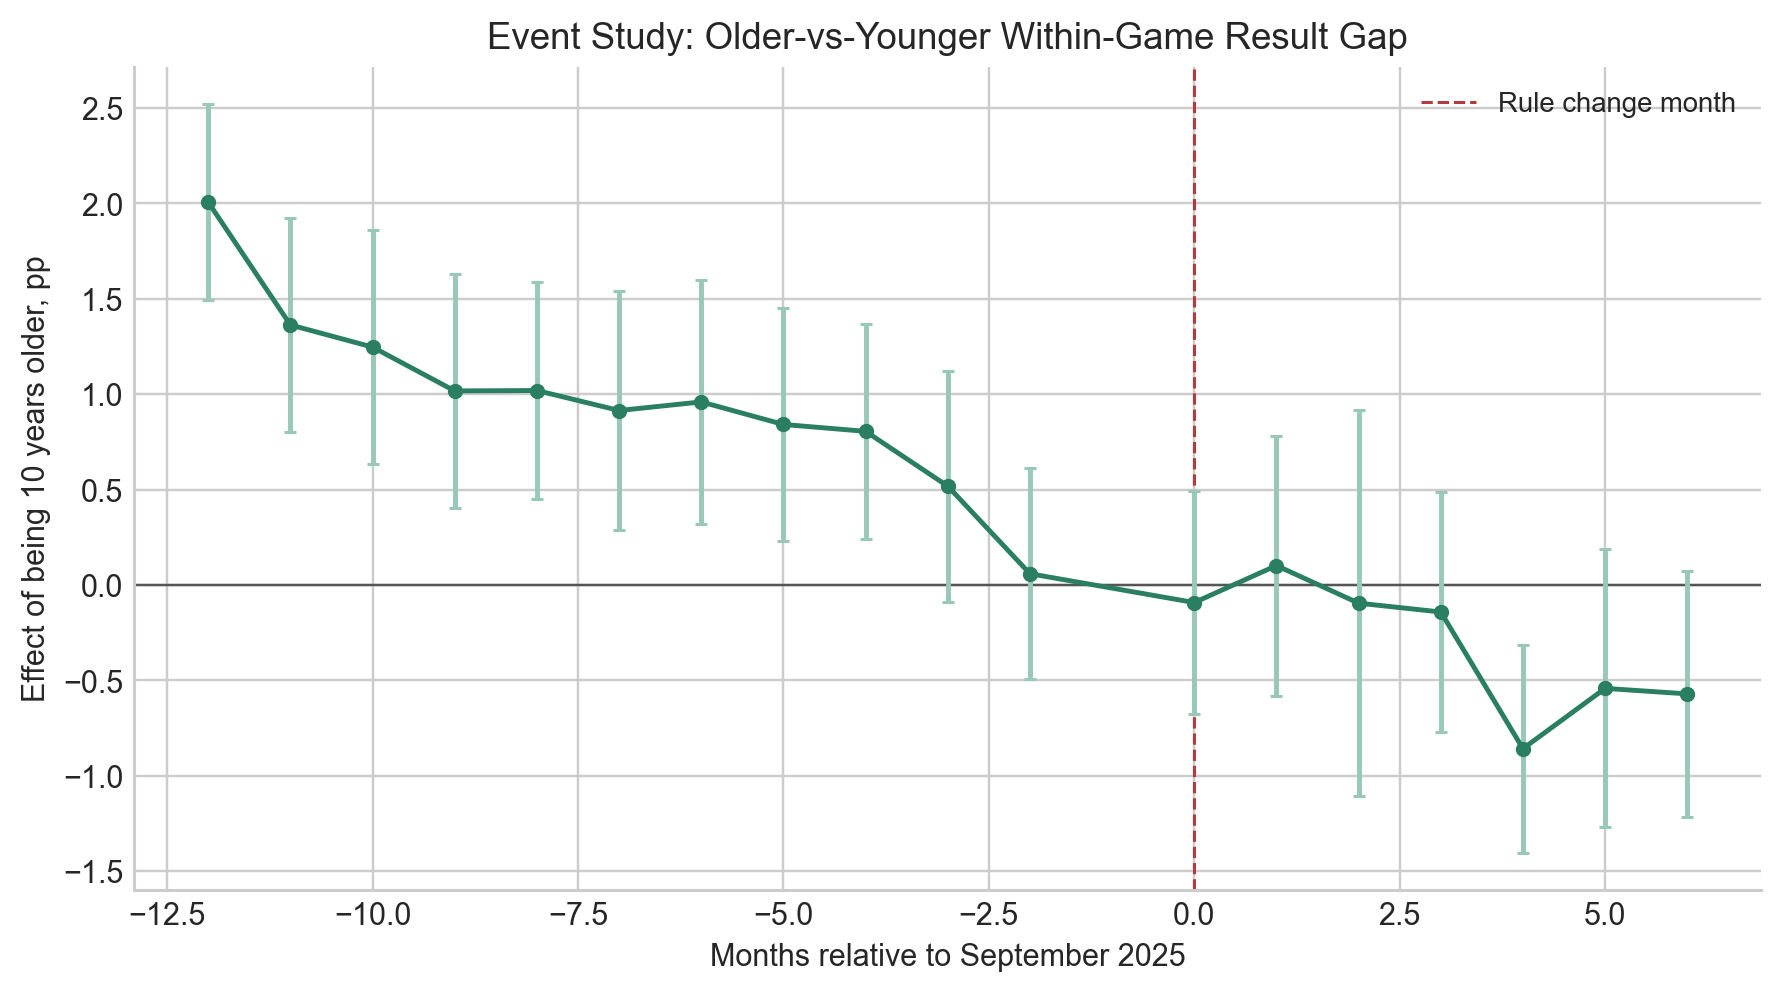
\includegraphics[width=0.90\textwidth]{figures/figure2_age_gap_event_study.png}
\caption{Event-study and coefficient pattern for the age-gap result.}
\label{fig:age-event-study}
\end{figure}

The caveat is that a September 2024 placebo cutoff also gives negative age effects, although smaller. For this reason, the thesis treats age as strong heterogeneity evidence and a plausible adaptability channel, not as a perfectly clean discontinuity. The most supported statement is descriptive: younger players gained relative to older players in the new format, and this pattern is visible in several within-player and within-game specifications.

\subsection{Time-Slot Displacement}

The reform removed the old late Titled Tuesday slot. Before the reform, the dataset contains 188 early-slot events and 187 late-slot events. After the reform, it contains 31 early-slot events and no late-slot events. This creates a second treatment margin: players who were late-slot regulars faced a larger schedule shock.

The time-slot evidence is strongest for participation and completion. Moving from a pure early-slot player to a pure late-slot player predicts a 13.3 percentage point lower probability of appearing after the reform and about 1.38 fewer post-reform tournaments out of 31 available. Conditional on returning, late regulars completed fewer rounds and had lower tournament score and rank. Table \ref{tab:timeslot} summarizes the main estimates.

\begin{table}[H]
\centering
\caption{Time-Slot Displacement Results}
\label{tab:timeslot}
\begin{adjustbox}{max width=\textwidth}
\begin{tabular}{llrrrl}
\toprule
Outcome & Treatment & Estimate & SE & p-value & Interpretation \\
\midrule
Any post-rule event & Pre late share & -0.133 & 0.018 & \(<0.001\) & Lower post participation \\
Number of post events & Pre late share & -1.376 & 0.163 & \(<0.001\) & Fewer post tournaments \\
Score after round 1 & Late regular & -0.0367 & 0.0094 & \(<0.001\) & Lower tournament score \\
Rank percentile & Late regular & -0.0397 & 0.0107 & \(<0.001\) & Worse final rank \\
Games after round 1 & Late regular & -0.0619 & 0.0145 & \(<0.001\) & Fewer games completed \\
Completed after round 1 & Late regular & -0.0741 & 0.0239 & 0.002 & Lower completion \\
Per-game result & Late regular & 0.0061 & 0.0095 & 0.522 & No clear game penalty \\
Per-game accuracy & Late regular & -0.097 & 0.143 & 0.500 & No clear accuracy penalty \\
\bottomrule
\end{tabular}
\end{adjustbox}
\end{table}

The important distinction is between tournament-level and game-level outcomes. Late regulars do worse in tournament score and rank because they participate less and complete fewer rounds. Conditional on sitting down to play a game, there is no clear evidence that they score worse or play less accurately. The schedule component therefore mainly affects selection and tournament completion.

\subsection{Field Composition, Pairing Structure, and Rank Movement}

The reform also changed the tournament environment. Event-level evidence shows that the field became smaller and more positively selected. Mean field rating rose by roughly 100 rating points in a raw interrupted-series model and by about 71 rating points when adding a calendar trend. Field size fell by roughly 97 players. These shifts matter because the post-change event is not simply the same population playing a different clock format.

Pairing structure also changed. Same-score pairings became less frequent, rating gaps narrowed, and pregame score gaps widened. Figure \ref{fig:rankmovement} shows rank movement by rating-advantage bin. The post-change tournament appears to reward rating advantage more strongly in final ranking as well as in individual game outcomes.

\begin{figure}[H]
\centering
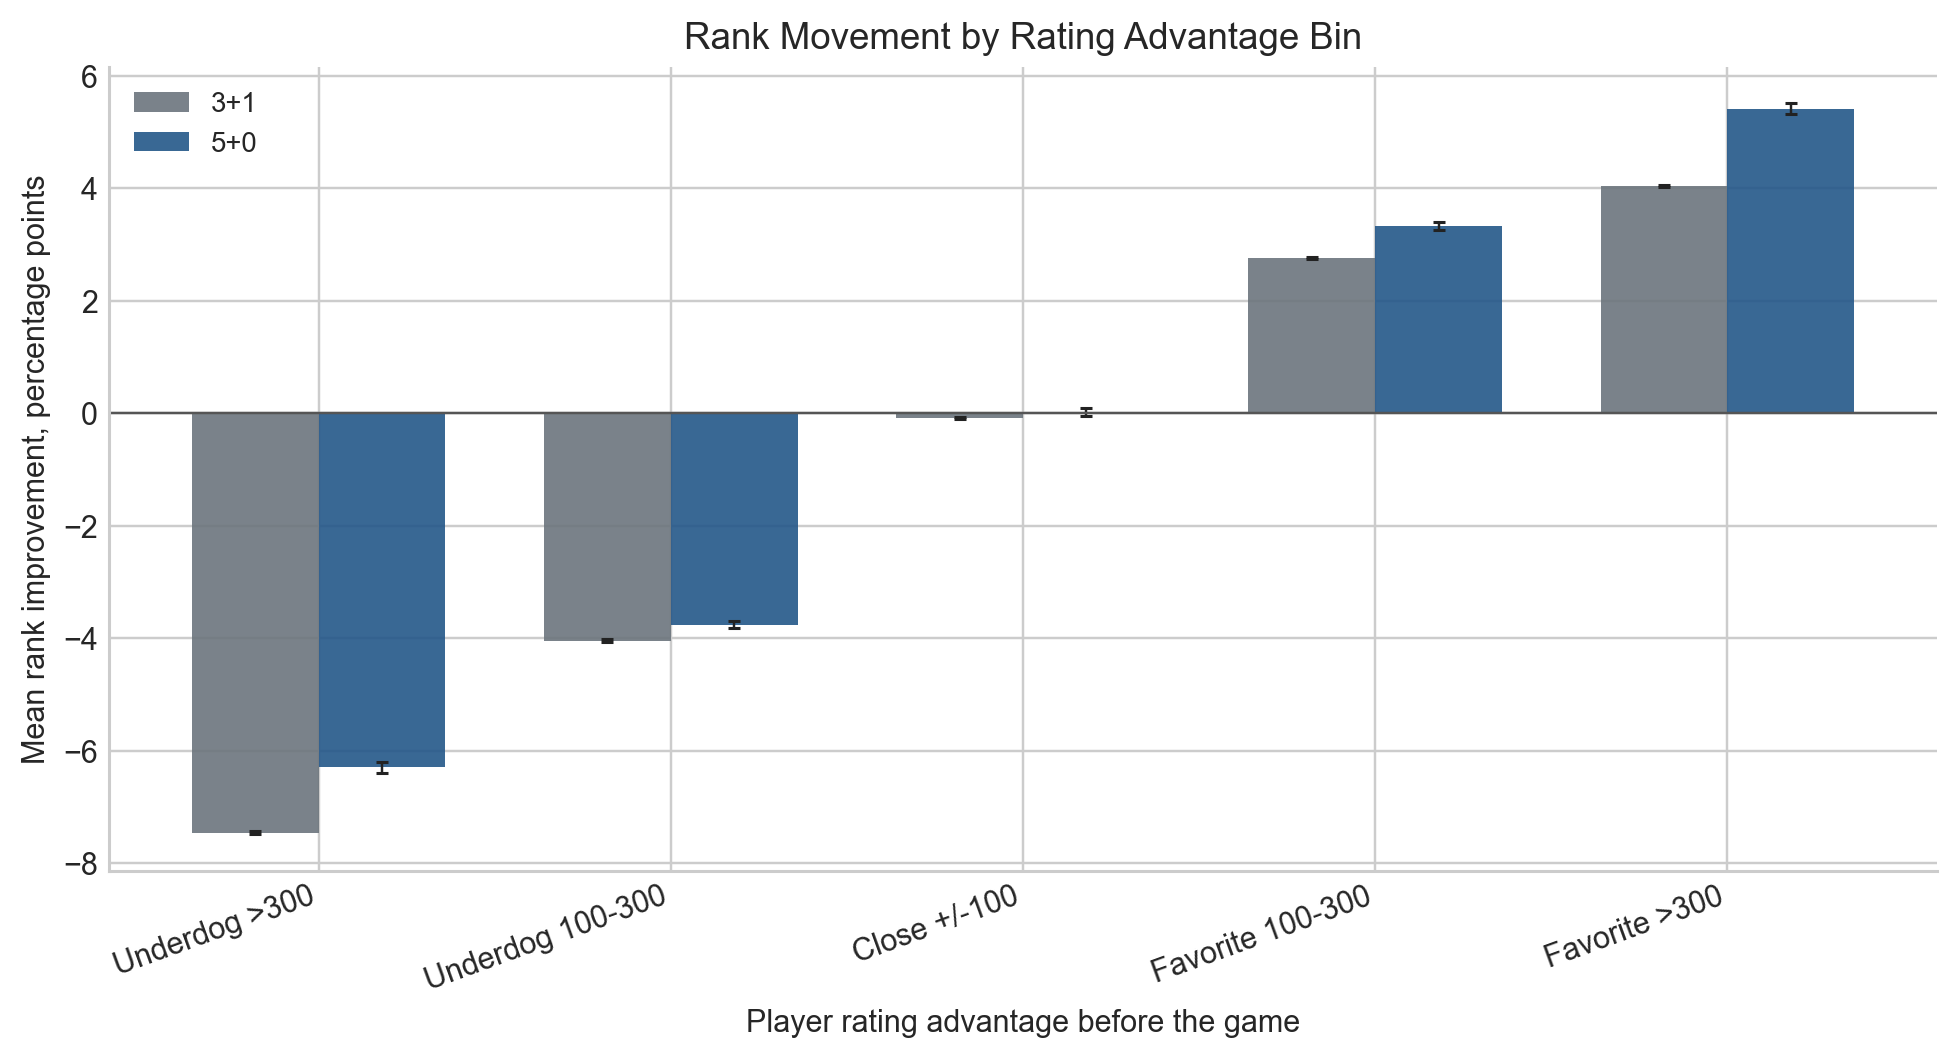
\includegraphics[width=0.90\textwidth]{figures/figure3_rank_movement_by_rating_advantage.png}
\caption{Pre/post rank movement by rating advantage.}
\label{fig:rankmovement}
\end{figure}

These field and pairing results are useful for interpretation. They show that the institutional reform changed both the production environment and the selection environment. The fixed-effect game-level models address conditional performance among observed games; the participation and field-composition results describe who appears in the new environment.

\subsection{Late-Game Error Accumulation}

Figure \ref{fig:stockfish-dashboard} summarizes the move-level mechanism evidence before reporting the individual estimates. The dashboard is useful because the main move-level interpretation does not come from a single coefficient: it comes from phase-specific error profiles, first-blunder timing, rating-bin conversion patterns, and deep conversion/recovery models.

\begin{figure}[H]
\centering
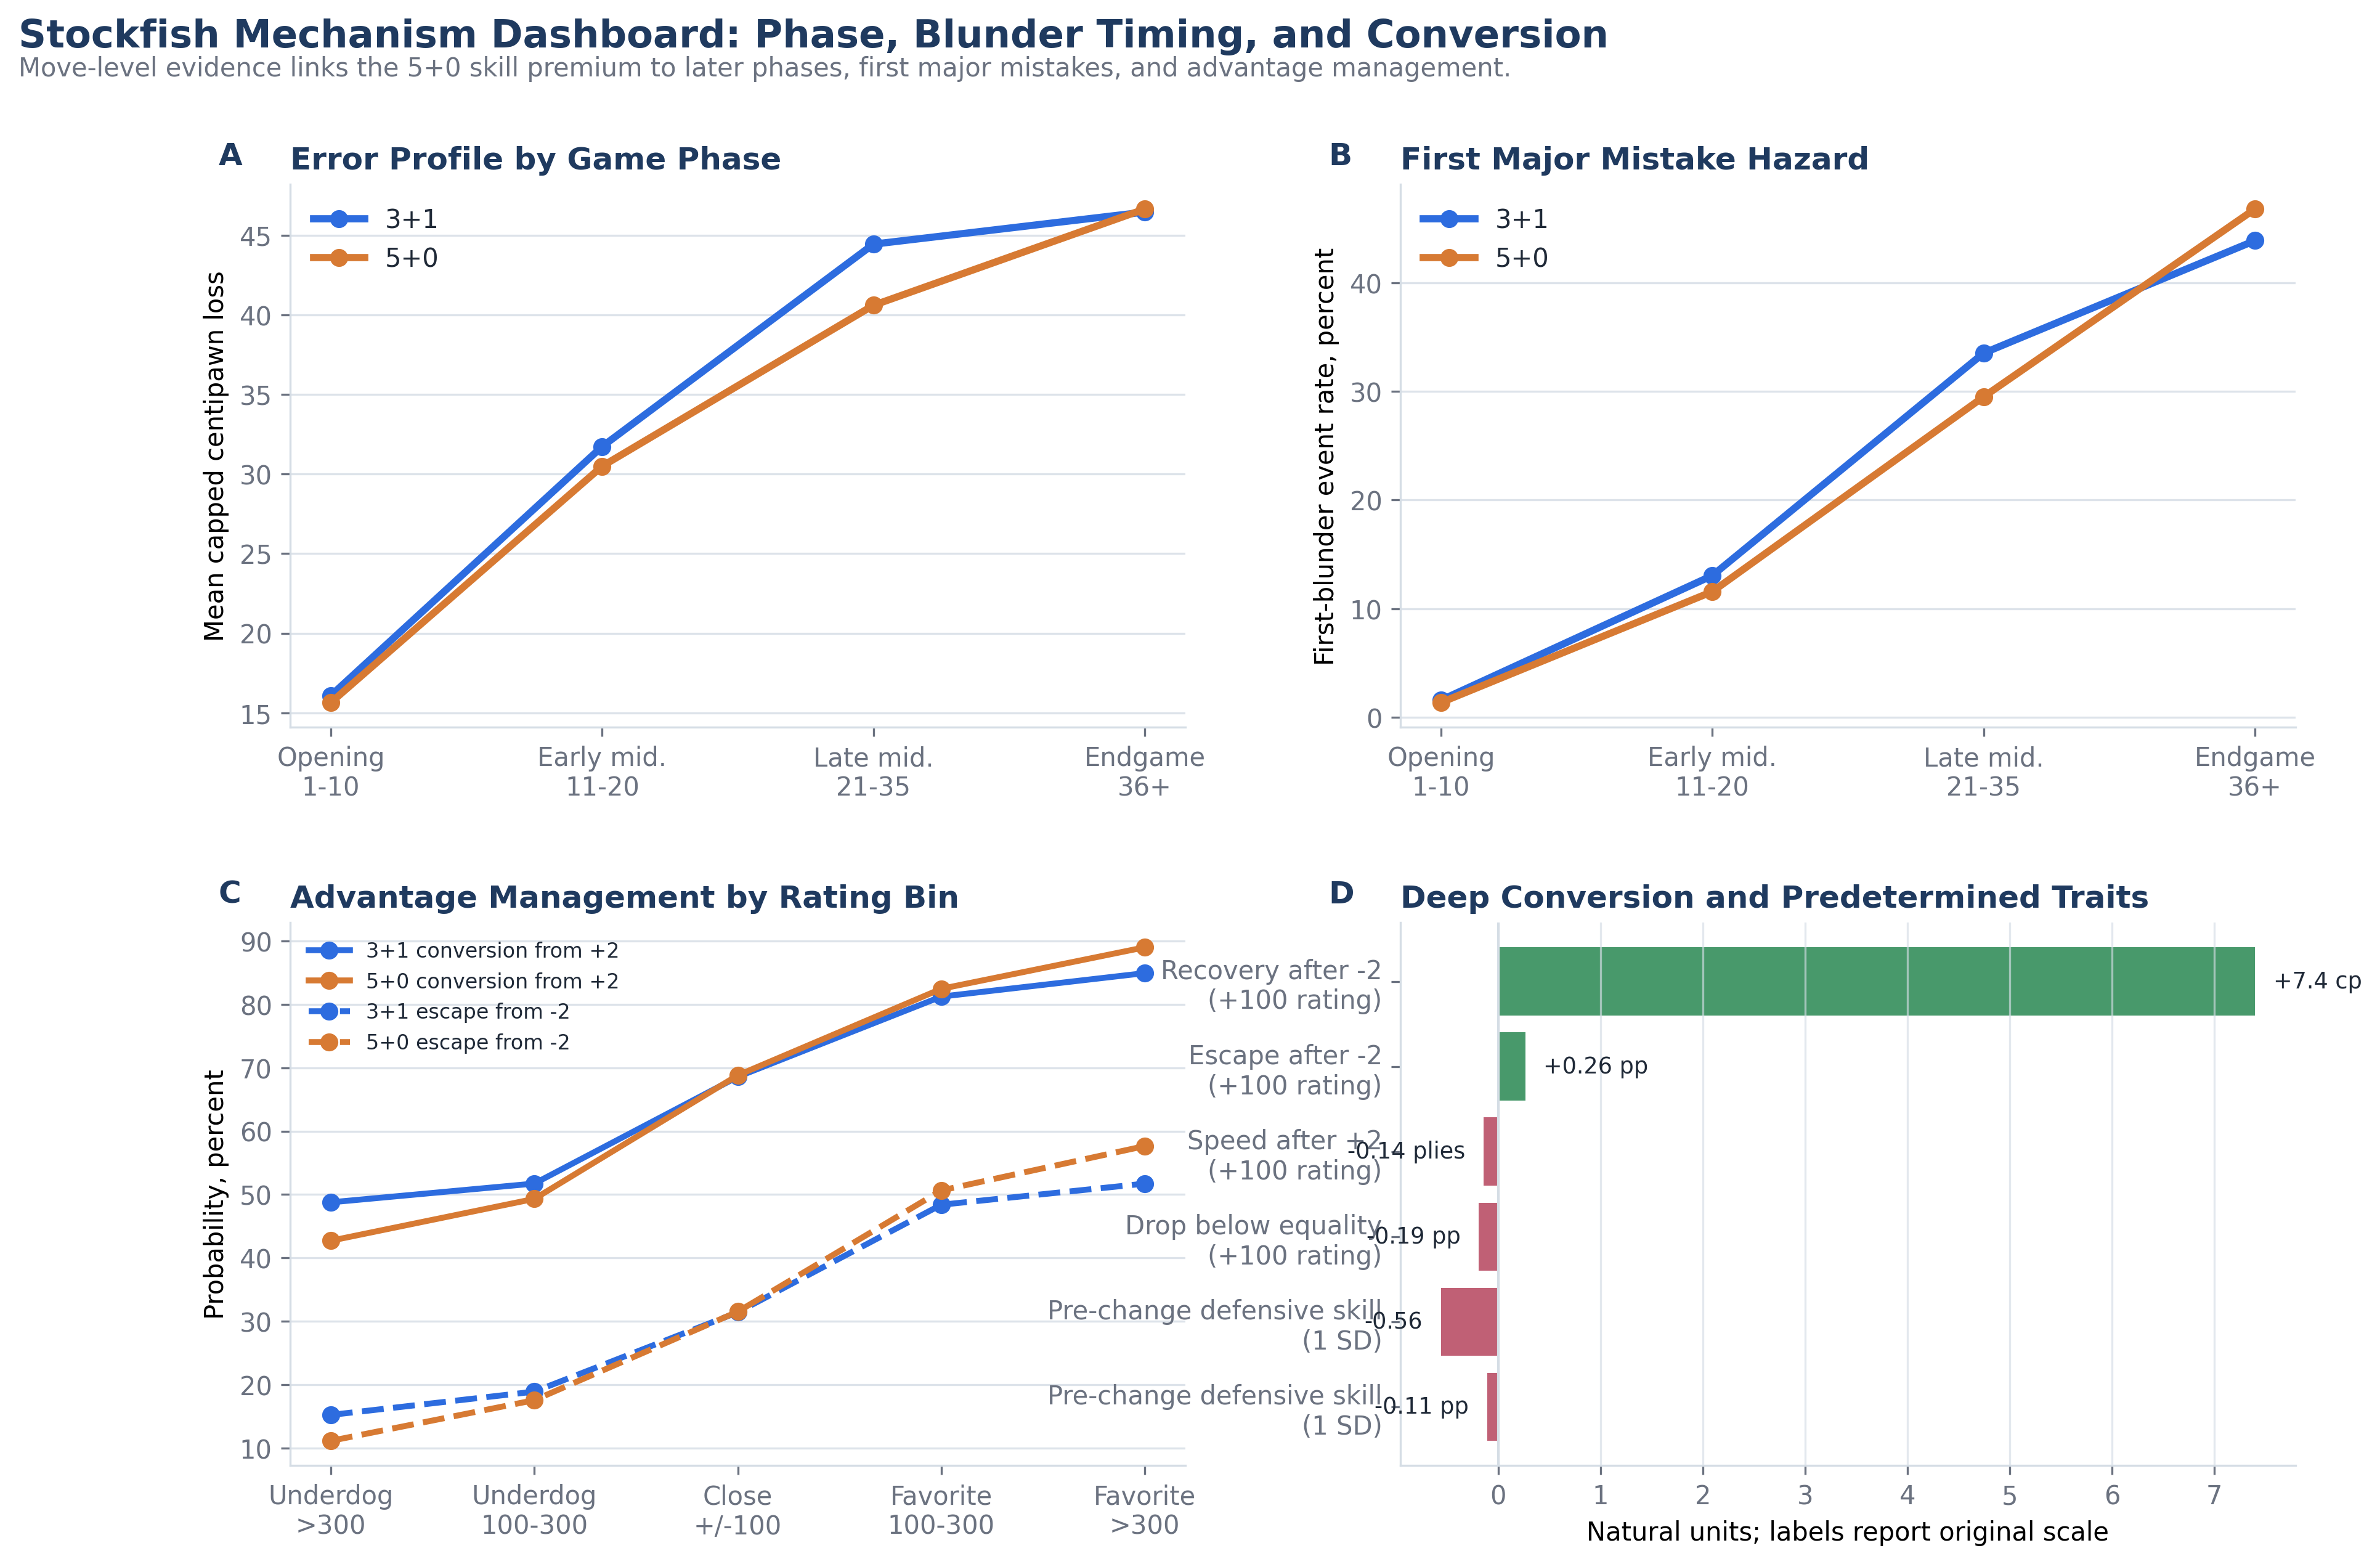
\includegraphics[width=\textwidth]{figures/figure9_stockfish_mechanism_dashboard.png}
\caption{Stockfish mechanism dashboard: phase errors, first-blunder hazard, conversion, and predetermined traits.}
\label{fig:stockfish-dashboard}
\end{figure}

The move-level Stockfish analysis shows that late phases became more costly under 5+0. The main phase model estimates \(\text{Post} \times \text{LatePhase}\) at about 2.06 capped centipawns. The final-ten-ply interaction is about 2.72 capped centipawns. These estimates are small in absolute centipawn terms, but they are estimated over more than 27 million moves and survive fixed effects and clustering. They indicate a systematic shift in where errors occur.

\begin{figure}[H]
\centering
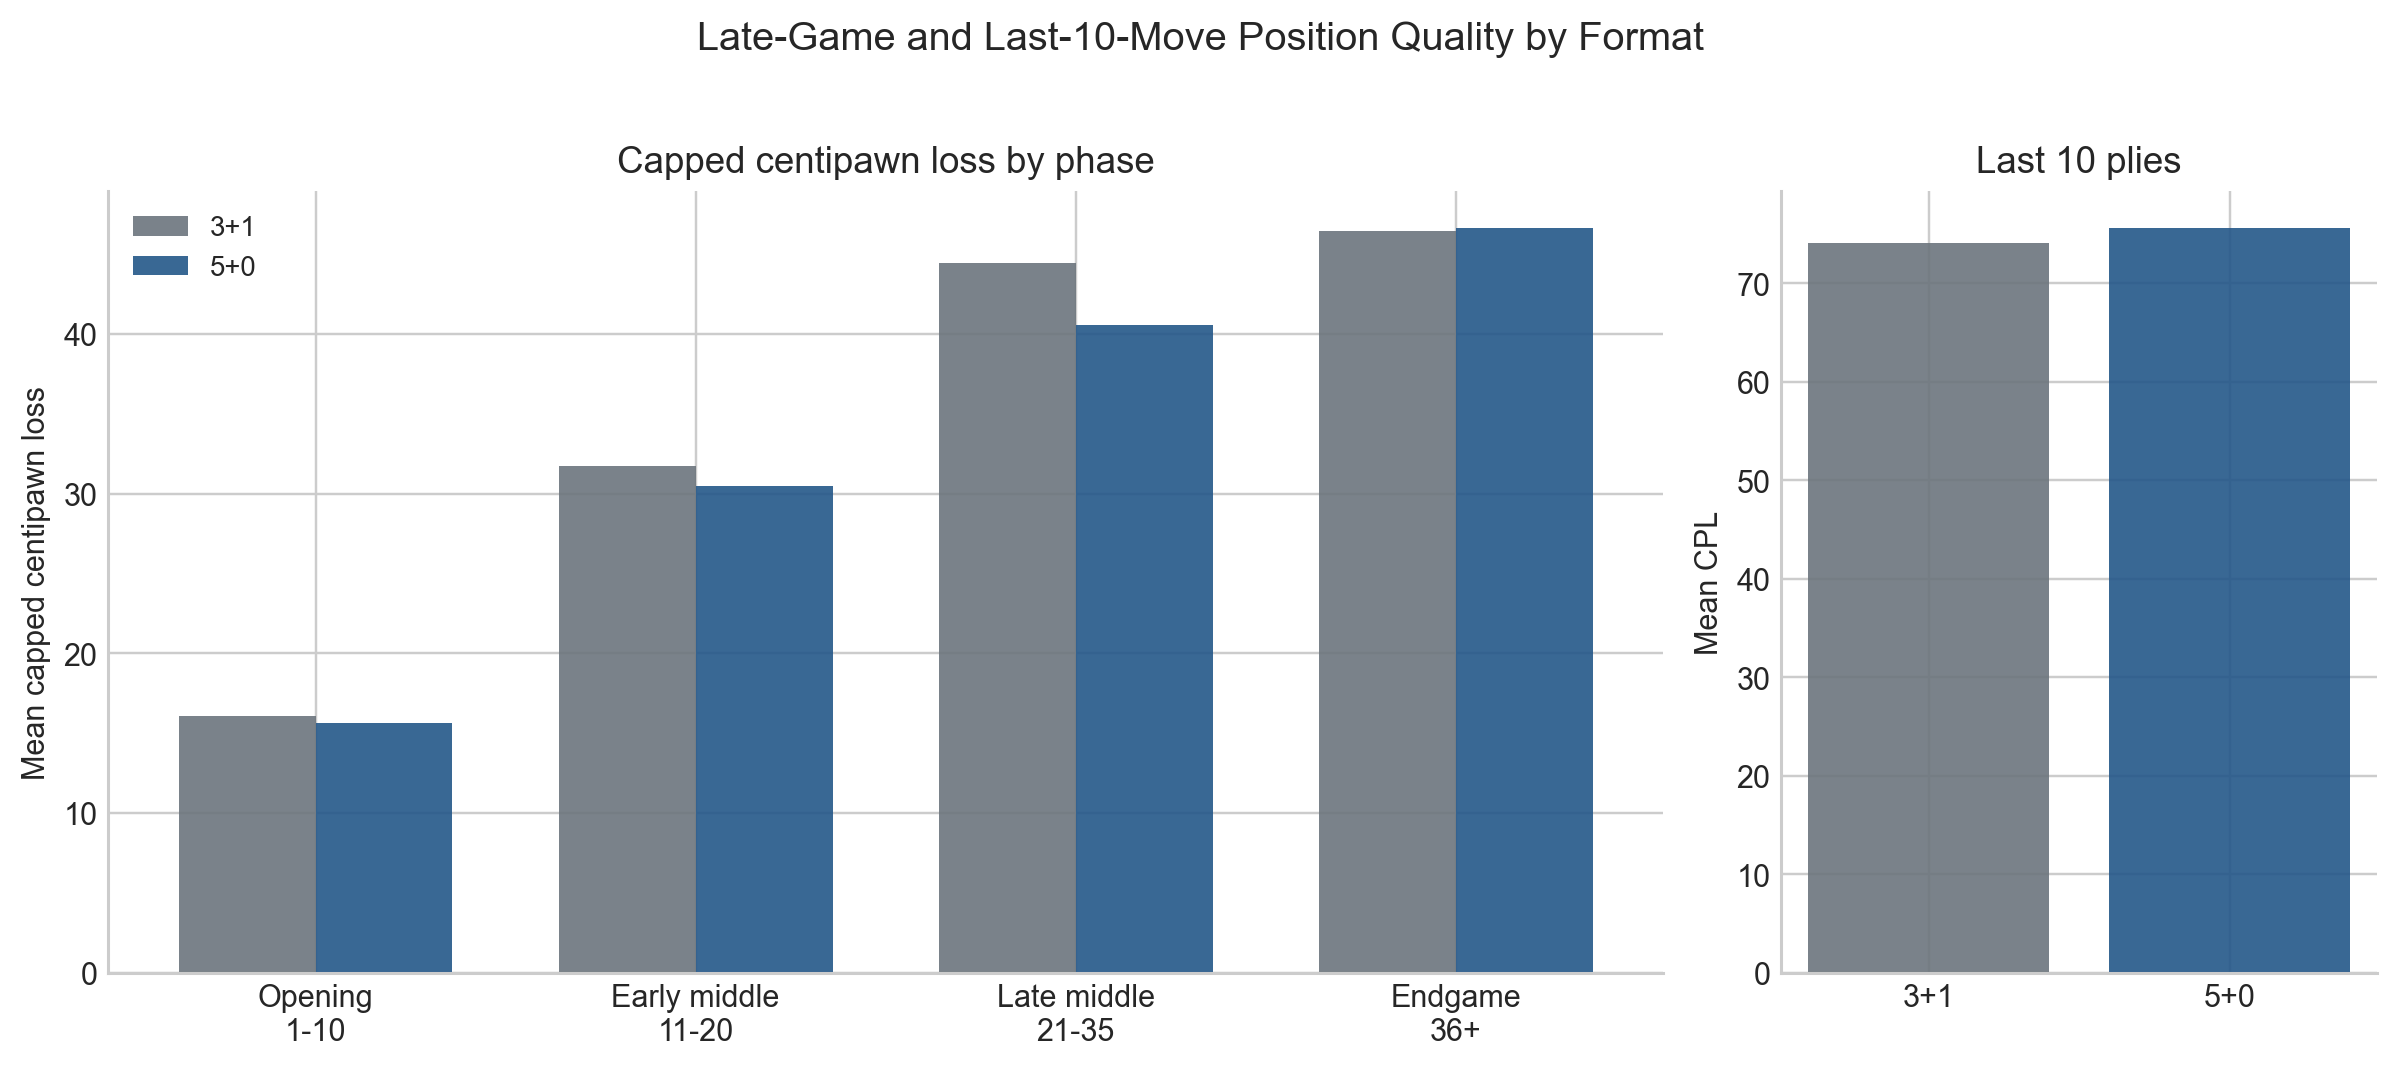
\includegraphics[width=0.90\textwidth]{figures/figure4_phase_last10_cp_loss.png}
\caption{Centipawn loss by phase and final-ten-ply status under 3+1 and 5+0.}
\label{fig:phasecpl}
\end{figure}

First-blunder hazard models show a related phase pattern. The post-change hazard falls in early and late middlegame phases but rises in endgames. The endgame phase interaction is about 0.0289. This phase result is complemented by the direct clock analysis below, which shows that the largest quality penalties are concentrated in severe low-clock states.

\subsection{Critical Positions and First Major Mistakes}

Critical or equal positions are defined as pre-move positions where the mover's engine evaluation is within 100 centipawns of equality. These positions are important because a single error can change the result expectation sharply. The post-change interaction on blunder probability in critical/equal positions is about 0.0020, or 0.20 percentage points. The corresponding capped-centipawn-loss estimate is about 0.75 centipawns.

Age heterogeneity appears in critical positions. The triple interaction \(\text{Post} \times \text{Age10} \times \text{CriticalEqual}\) is about 0.27 capped centipawns, and the triple interaction in blunder probability is positive as well. These estimates suggest that older players face a larger post-change penalty in tactically sensitive equal positions, though the strongest age evidence remains at the player-game level and in first-blunder timing.

First-blunder timing gives another view of how errors are distributed within games. Conditional on having a blunder, a player 10 years older blundered about one-third of a move earlier after the reform. Female players blundered about one move earlier conditional on blundering, but broad female move-level interactions are not robust enough to support a general female-specific deterioration story. The no-blunder-game probability by age is weaker after multiple-testing adjustment, so first-blunder timing is the preferred error-timing result.

\subsection{Clock-Time Mechanisms}

The clock data refine the interpretation of the move-level results. The simple story would be that 5+0 mechanically creates more time pressure. This is not what the data show. Because the new format gives each player five initial minutes instead of three, ordinary low-clock exposure actually falls. The share of moves started with 10 seconds or less falls from about 10.0\% before the reform to 3.8\% after the reform, and the mean final clock rises from 33.3 seconds to 64.7 seconds. Figure \ref{fig:clock-exposure-insurance} visualizes this shift. The important change is therefore not the average amount of time pressure, but the technology of severe time pressure. In 3+1, a player who reaches a very low clock can sometimes rebuild time through the one-second increment. In 5+0, recovery is essentially impossible.

\begin{figure}[H]
\centering
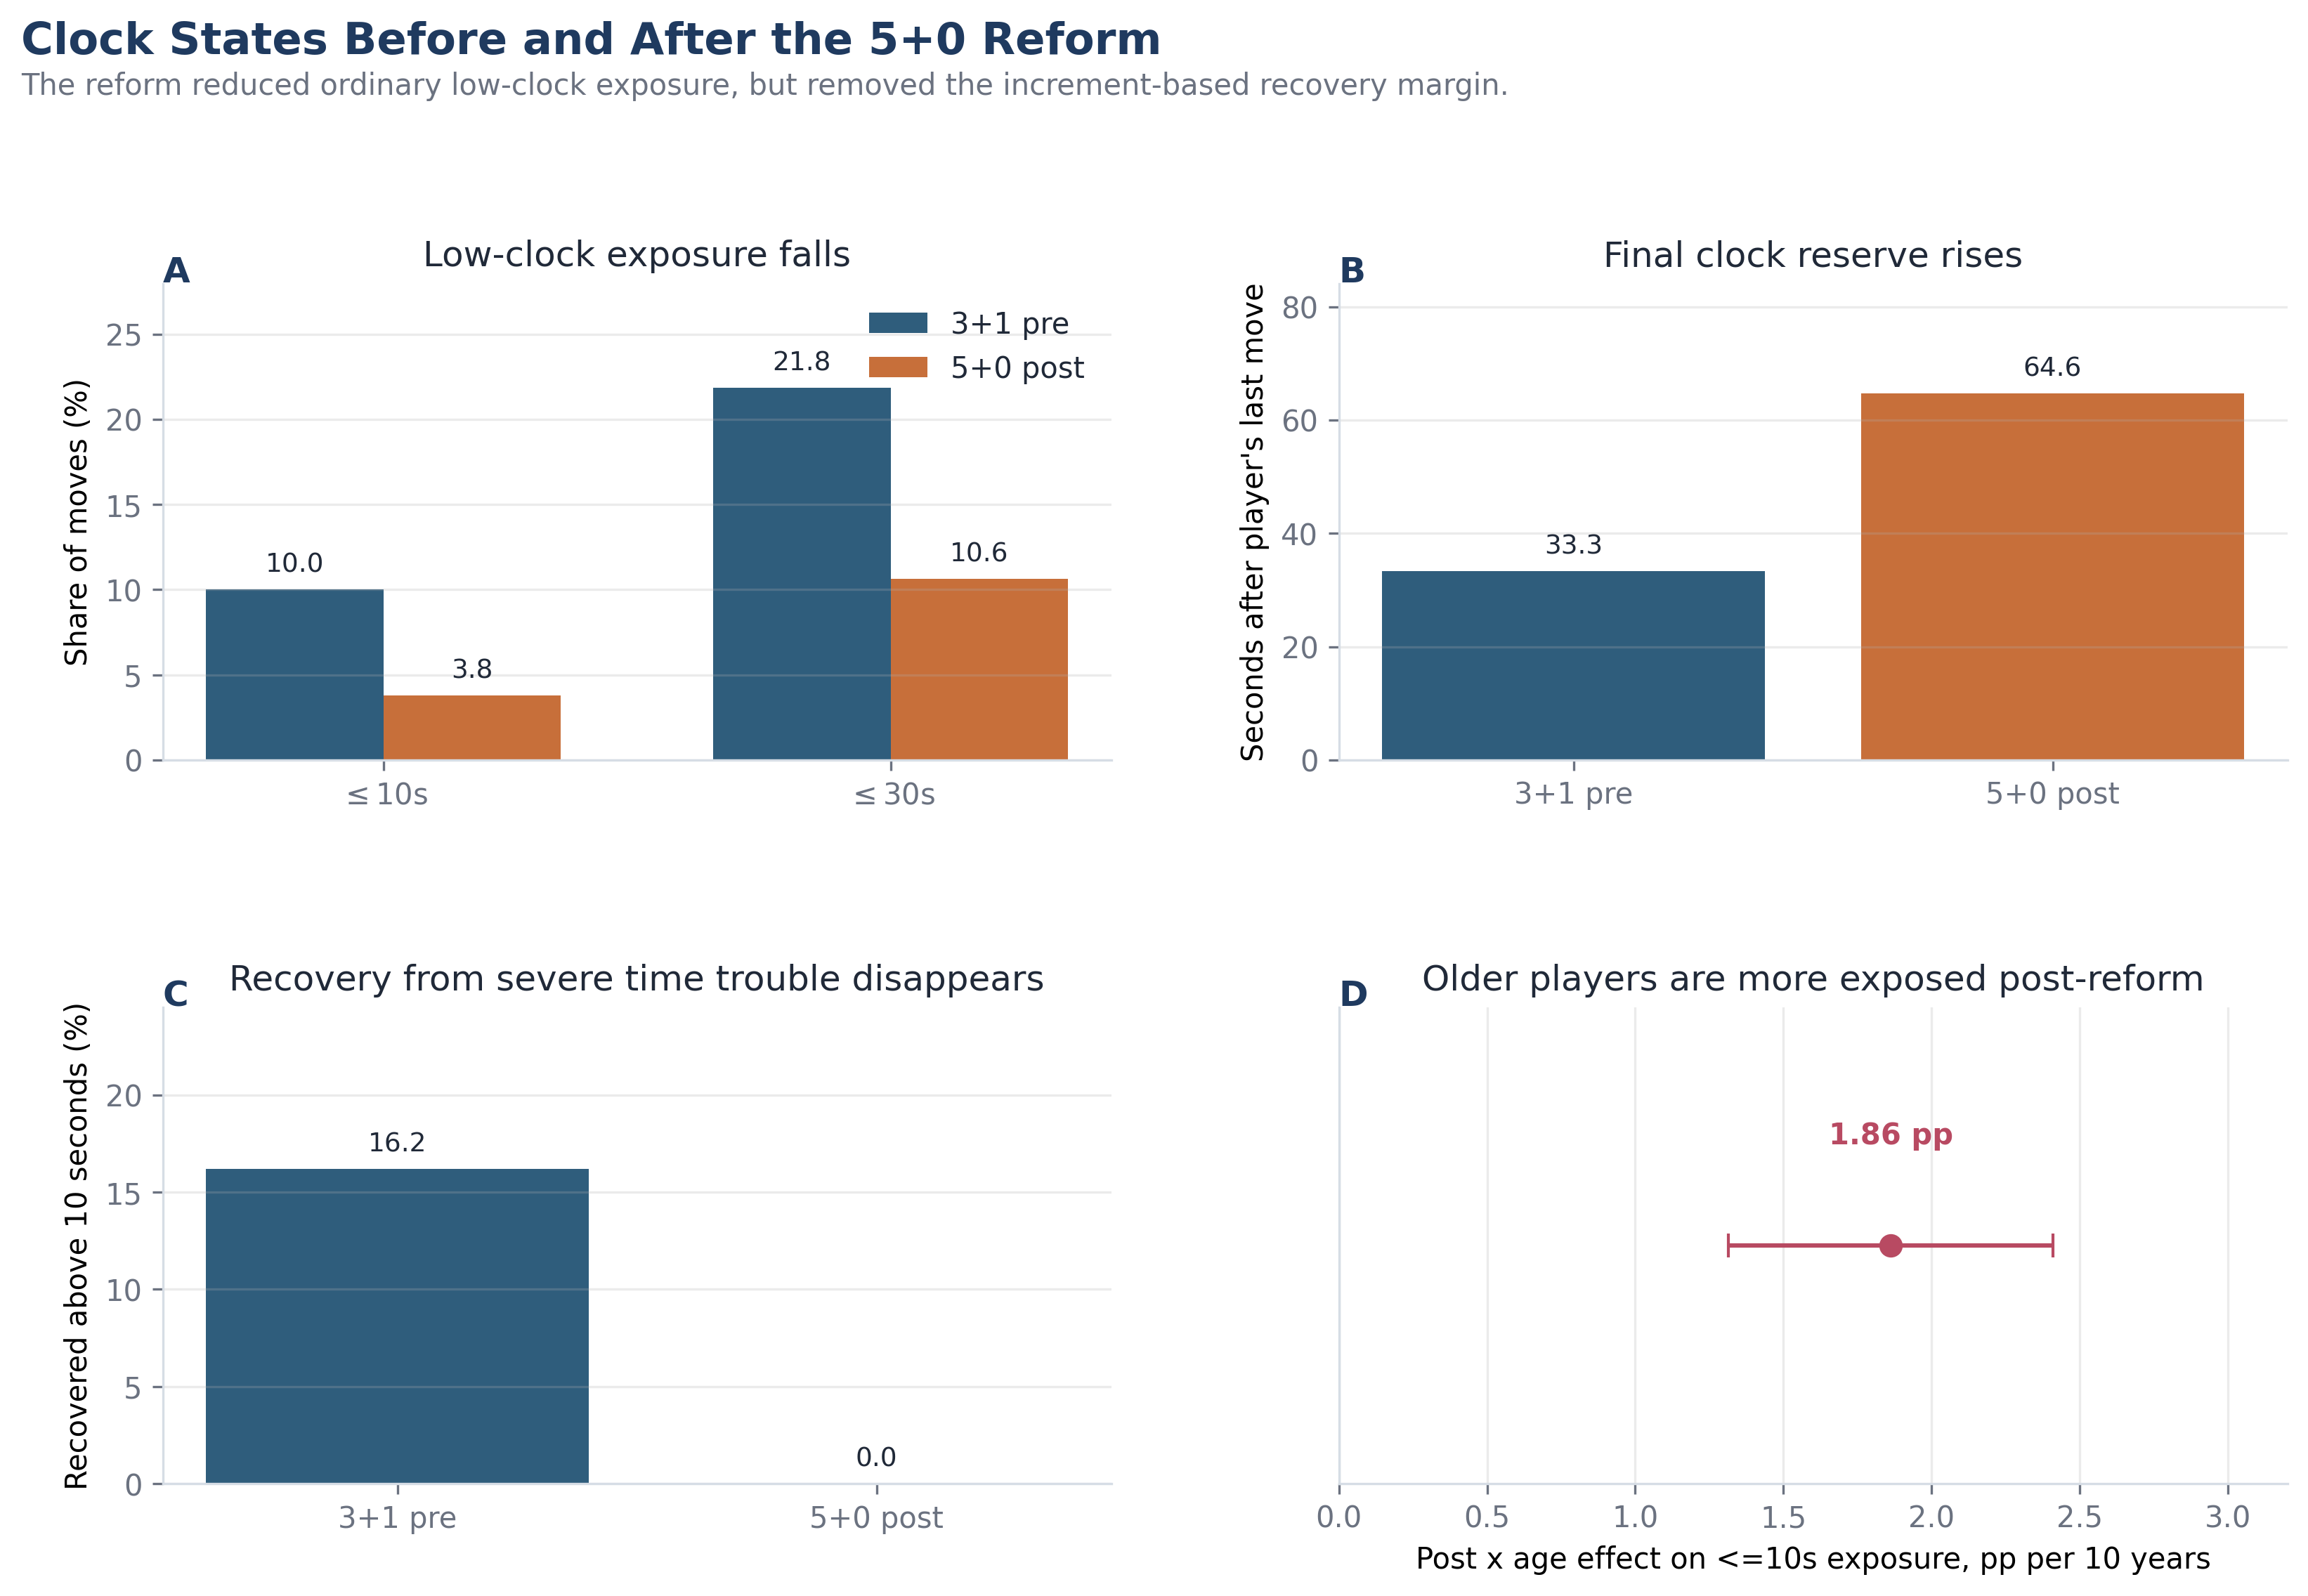
\includegraphics[width=\textwidth]{figures/figure12_clock_exposure_insurance.png}
\caption{Clock states before and after the reform: low-clock exposure, final clock reserve, low-clock recovery, and age heterogeneity.}
\label{fig:clock-exposure-insurance}
\end{figure}

\begin{table}[H]
\centering
\caption{Robust Clock-Time Mechanisms}
\label{tab:clock-mechanisms}
\small
\begin{adjustbox}{max width=\textwidth}
\begin{tabular}{p{0.24\textwidth}p{0.25\textwidth}p{0.18\textwidth}p{0.24\textwidth}}
\toprule
Mechanism & Main estimate & Significance & Interpretation \\
\midrule
Lower ordinary low-clock exposure & Post effect on share of moves starting with \(\leq 10\) seconds: \(-0.0734\) & \(p<0.001\) & Players reach very low clock less often because 5+0 starts with a larger time budget. \\
Higher cost of severe time trouble & Post interaction for \(\leq 10\)-second exposure: \(+19.82\) capped centipawns; exact bin interactions: \(+14.87\) cp for 5--10s and \(+29.15\) cp for 0--5s & \(p<0.001\) & Once severe time trouble occurs, move quality deteriorates much more under 5+0. \\
Loss of increment insurance & Post effect on recovery above 10 seconds after entering \(\leq 10\) seconds: \(-0.1648\) & \(p<0.001\) & Under 3+1 some players rebuild time; under 5+0 this margin essentially disappears. \\
Clock weakness and conversion & Own low clock at first winning position: post penalty about \(-0.29\); opponent low clock at first winning position: post gain about \(+0.10\); opponent low clock when worse: post escape gain about \(+0.30\) & \(p<0.001\) & Low own clock makes winning positions harder to convert, while opponent clock weakness becomes a valuable practical resource. \\
Age and clock adaptation & Post-by-age effect on \(\leq 10\)-second exposure: \(+0.0186\) per 10 years & \(p<0.001\) & Older players are relatively more exposed to very low-clock states after the reform. \\
\bottomrule
\end{tabular}
\end{adjustbox}
\end{table}

These estimates support a specific mechanism. The no-increment format does not simply make every move faster or noisier. It reduces the frequency of ordinary low-clock states but increases the marginal cost of reaching extreme time trouble. The exact move-bin regressions show that the post-change penalty is small or negative in moderate clock bins, but rises sharply below 10 seconds. Event-time models around the first low-clock crossing lead to the same conclusion: first crossing below 30 seconds does not generate a persistent post-change error cascade, while first crossing below 10 seconds does. Figure \ref{fig:clock-panic-conversion} shows both the panic-threshold pattern and the conversion role of own and opponent low-clock states.

\begin{figure}[H]
\centering
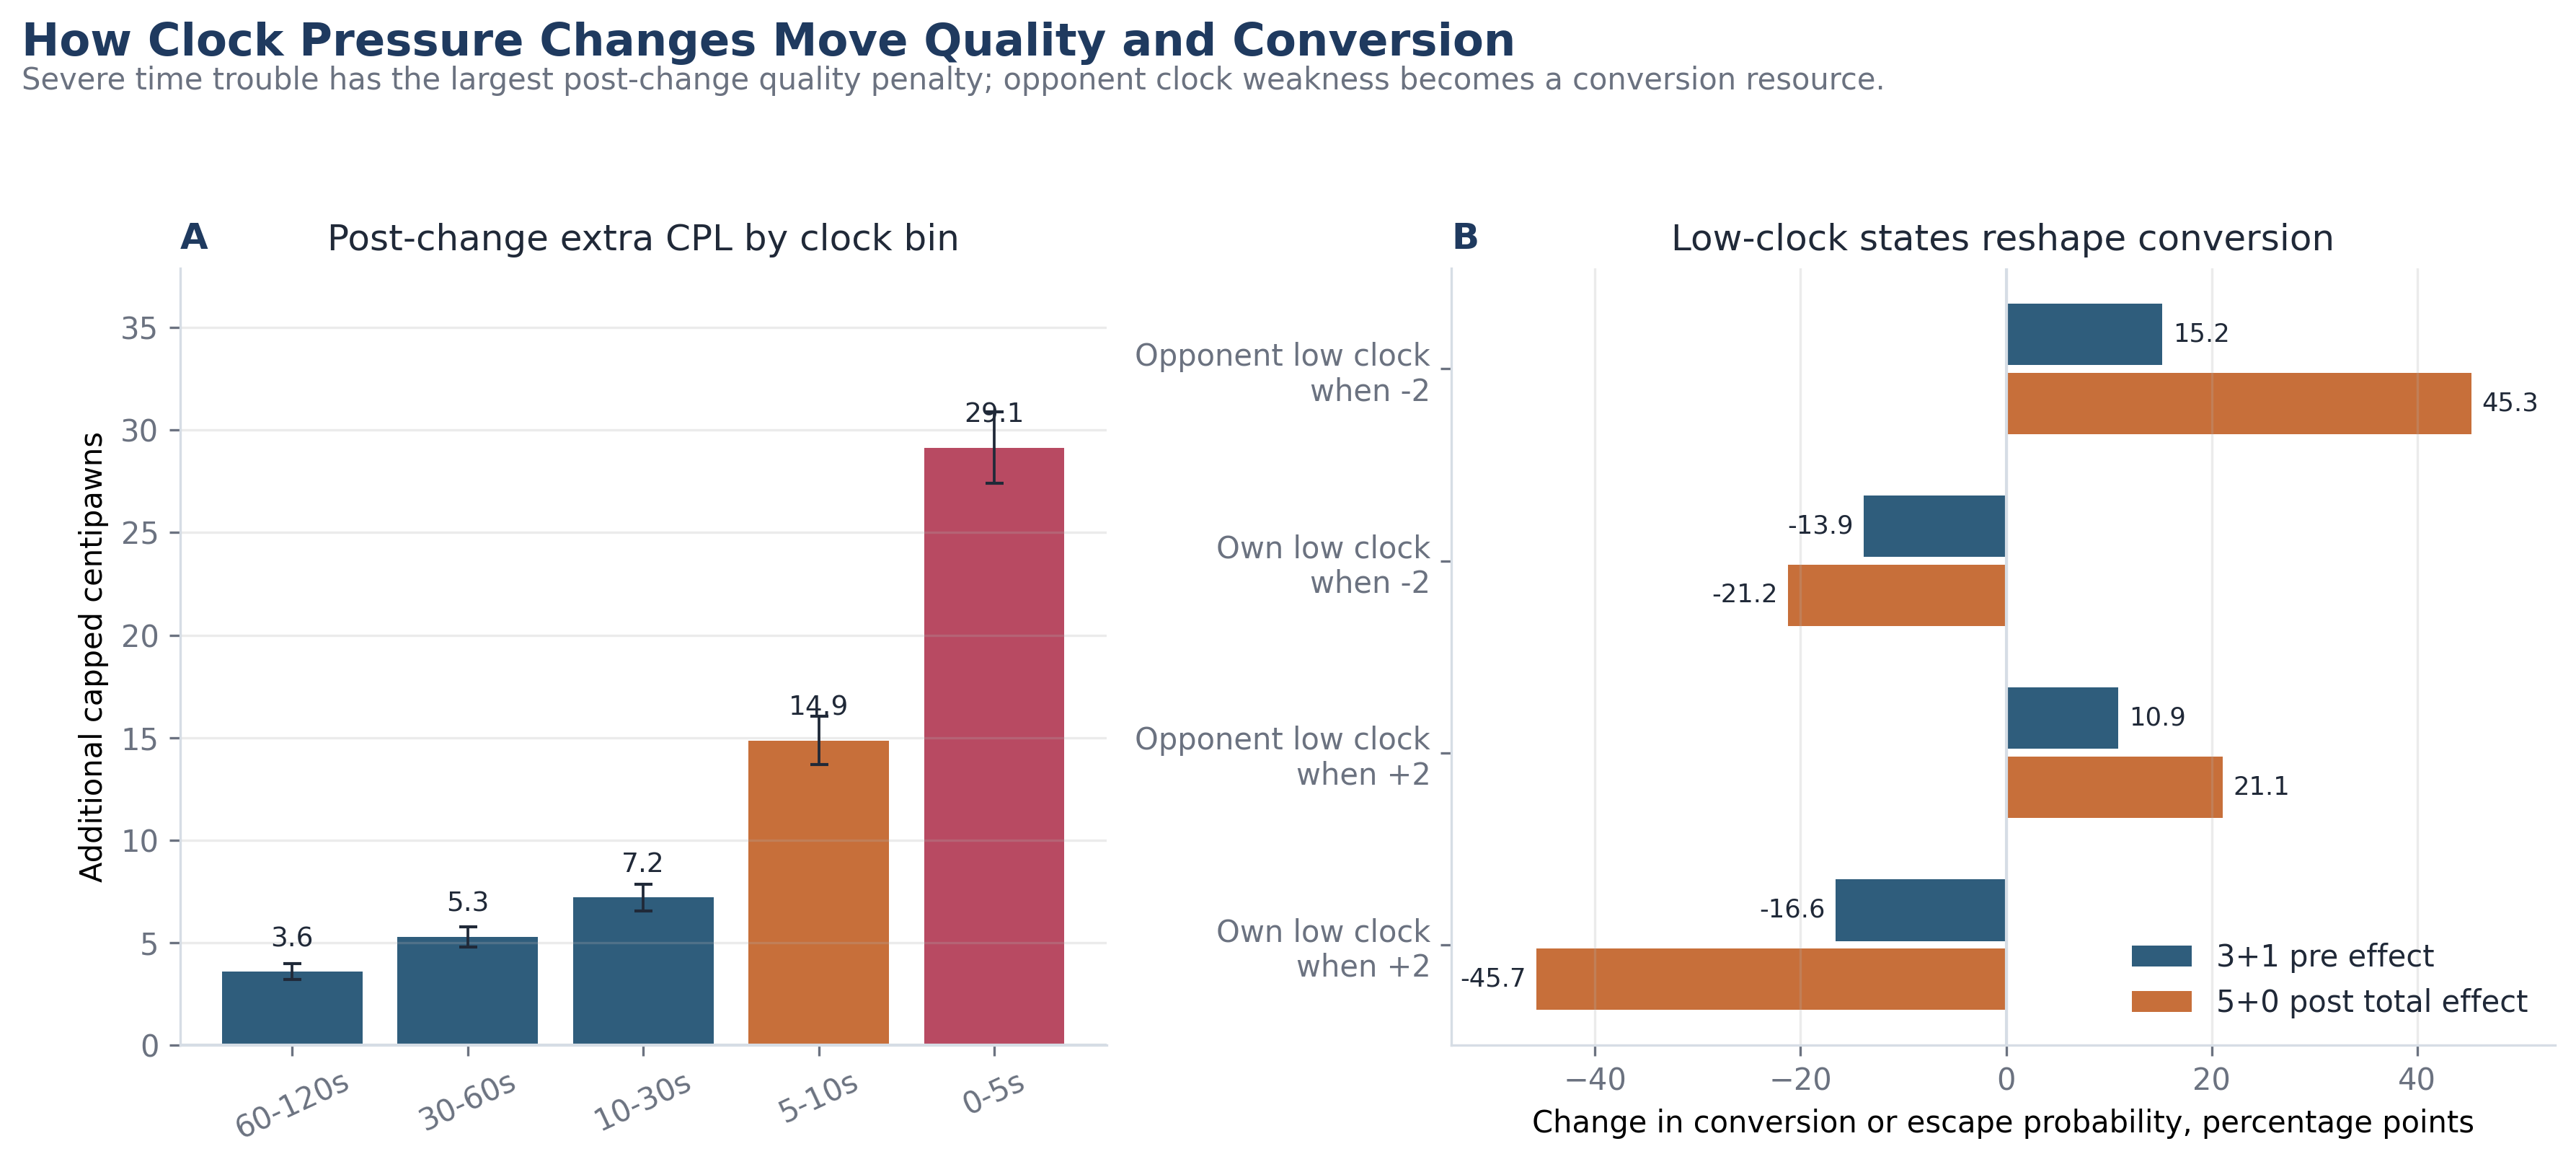
\includegraphics[width=\textwidth]{figures/figure13_clock_panic_conversion.png}
\caption{Clock pressure mechanisms: post-change centipawn-loss penalties by clock bin and low-clock effects on conversion or defensive escape.}
\label{fig:clock-panic-conversion}
\end{figure}

Clock states also change conversion technology. When a player first reaches a winning engine position while personally below 10 seconds, conversion becomes much harder after the reform. Conversely, if the opponent is already below 10 seconds when the player reaches a winning or losing engine state, the player converts or escapes much more often. This result connects the clock analysis to the main skill-premium result: under 5+0, objective board advantage, engine-measured accuracy, and clock capital jointly determine whether advantages become points.

\subsection{Conversion From Winning Positions and Defensive Recovery}

The conversion results connect the game-level skill premium to concrete move-level mechanisms. Winning positions are defined as positions where the player reached at least +200 centipawns from the engine's perspective at least ten plies before the game ended. A stronger rating advantage increased post-change conversion from winning positions by about 0.33 percentage points per 100 rating points. The defensive escape model is also positive: a 100-point rating advantage increased post-change escape from losing positions by about 0.40 percentage points.

\begin{table}[H]
\centering
\caption{Move-Level and Conversion Mechanisms}
\label{tab:move-mechanisms}
\begin{adjustbox}{max width=\textwidth}
\begin{tabular}{llrrrl}
\toprule
Result & Outcome & Estimate & SE & p-value & Unit \\
\midrule
Late phase error & Capped CPL & 2.0566 & 0.3245 & \(<0.001\) & Endgame, fullmove 36+ \\
Last-10-ply error & Capped CPL & 2.7231 & 0.4975 & \(<0.001\) & Final 10 plies \\
Critical/equal blunder & Blunder probability & 0.0020 & 0.0003 & \(<0.001\) & \(|eval|<100\) cp \\
Critical/equal CPL & Capped CPL & 0.7466 & 0.1795 & \(<0.001\) & \(|eval|<100\) cp \\
Winning conversion & Converted +2 & 0.0033 & 0.0007 & \(<0.001\) & Per +100 rating advantage \\
Defensive escape & Escaped -2 & 0.0040 & 0.0008 & \(<0.001\) & Per +100 rating advantage \\
Conversion speed & Plies to conversion & -0.1425 & 0.0302 & \(<0.001\) & Per +100 rating advantage \\
Recovery after -2 & Recovery probability & 0.0026 & 0.0006 & \(<0.001\) & Per +100 rating advantage \\
First blunder by age & First blunder move & -0.3315 & 0.0735 & \(<0.001\) & Per +10 years \\
\bottomrule
\end{tabular}
\end{adjustbox}
\end{table}

The deeper conversion results are especially informative. After reaching +2, stronger players converted faster under 5+0: the estimate is -0.1425 plies per 100 rating points. They were also less likely to drop the position back below equality, with an estimate of -0.0019 per 100 rating points. After reaching -2, stronger players recovered more, gaining about 7.4 centipawns more in the recovery measure and increasing recovery probability by about 0.26 percentage points per 100 rating points.

\begin{figure}[H]
\centering
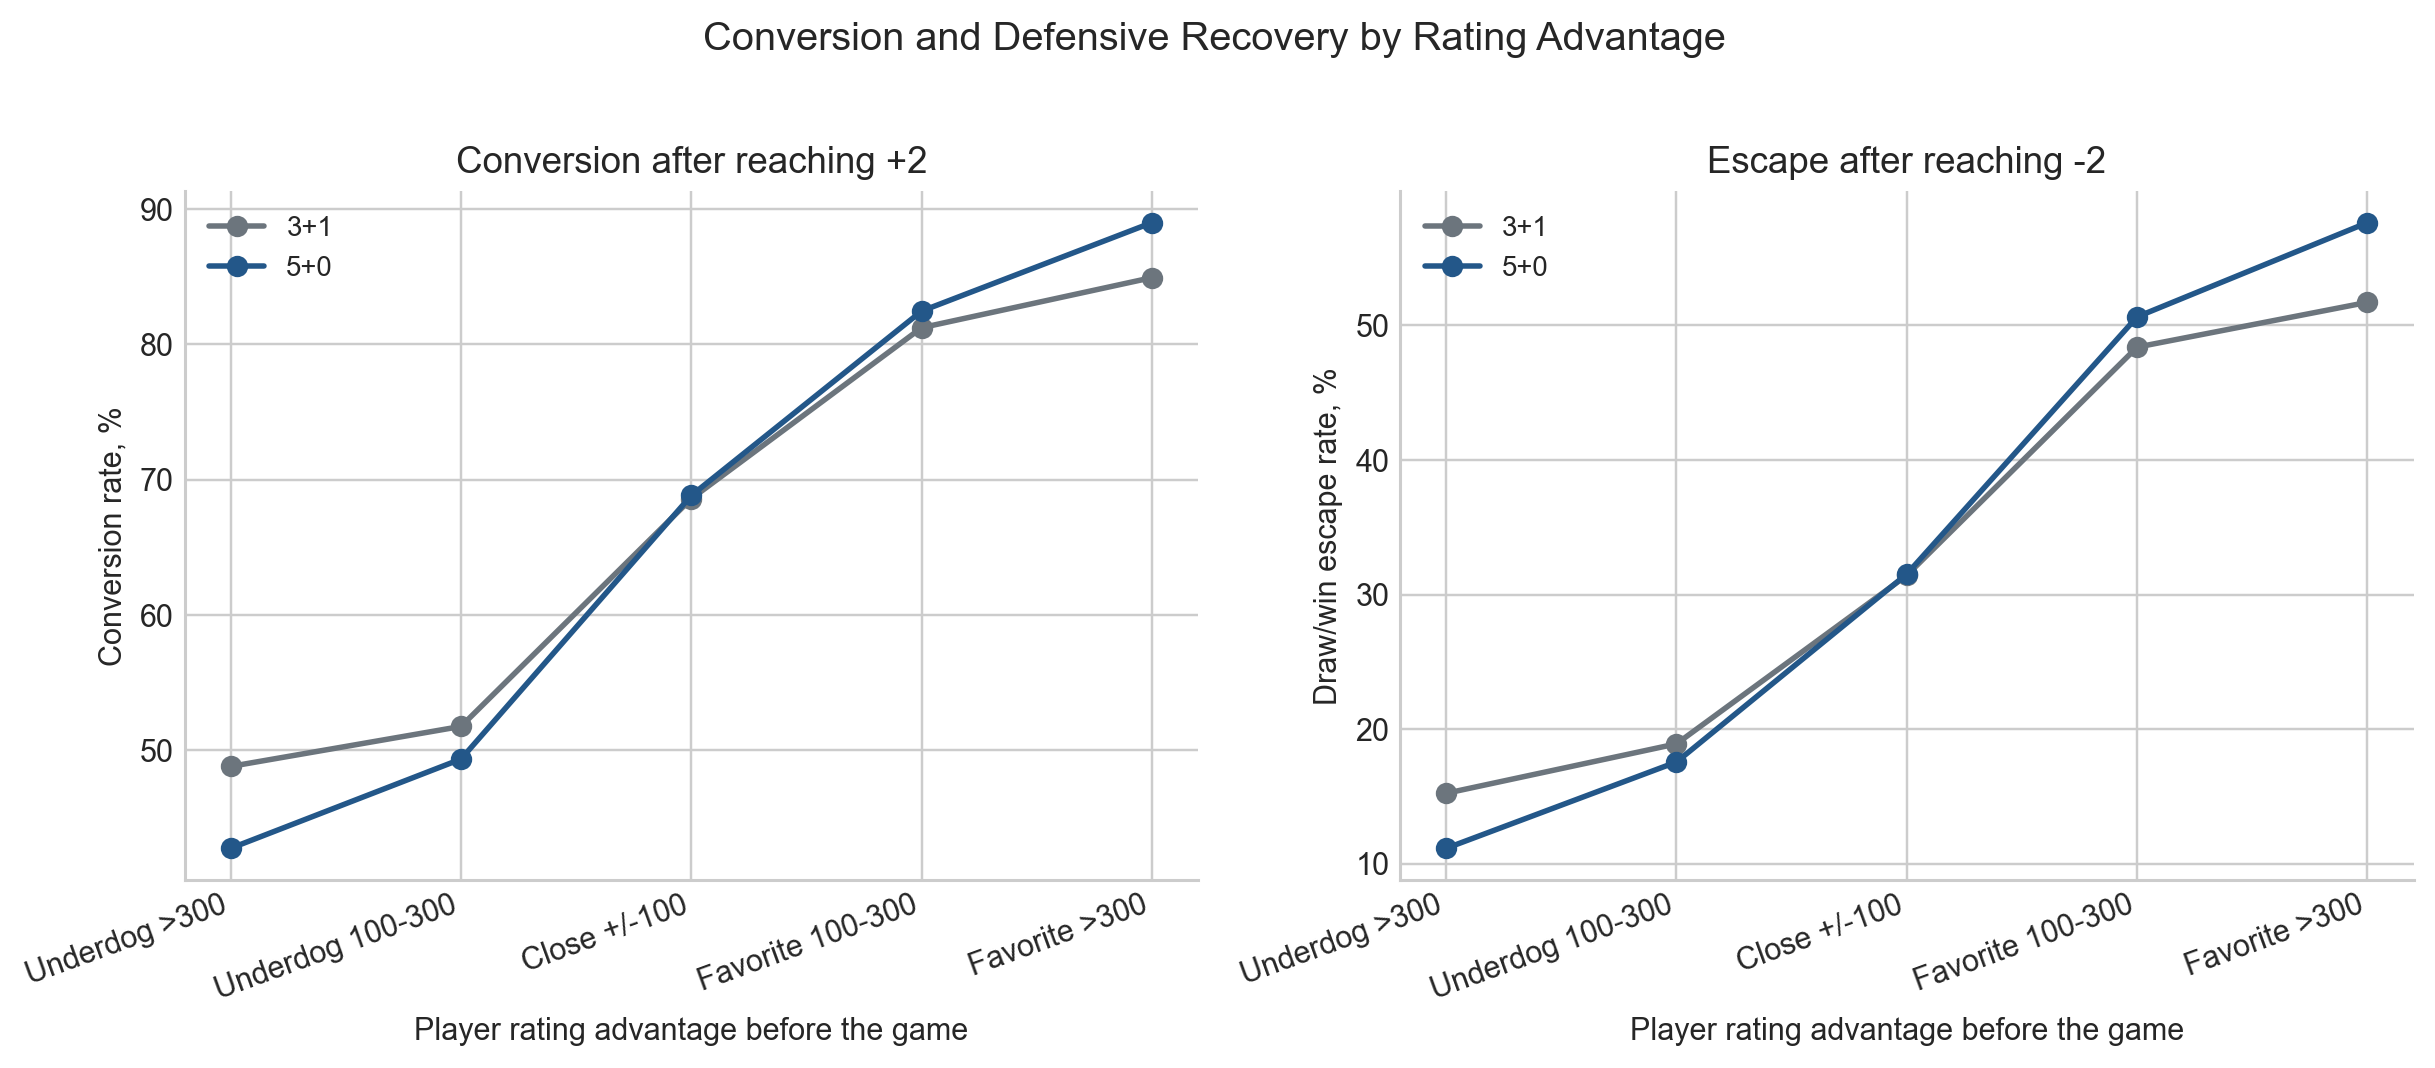
\includegraphics[width=0.90\textwidth]{figures/figure5_conversion_recovery_by_rating_advantage.png}
\caption{Conversion from +2 and recovery from -2 by rating advantage.}
\label{fig:conversion}
\end{figure}

Together these results show that the post-change skill premium is not just a rating-table artifact. It appears in advantage management. Stronger players convert winning positions more efficiently, lose fewer advantages, and recover more from worse positions under the no-increment format.

\subsection{Complexity and Predetermined Skill Traits}

The complexity results are nuanced. The data do not show that all complex positions became uniformly worse under 5+0. Instead, complexity moderates who benefits. The interaction \(\text{Post} \times \text{ComplexityIndex}\) in capped centipawn loss is negative, while the triple interaction \(\text{Post} \times \text{Age10} \times \text{ComplexityIndex}\) is positive. This means that complex positions were not simply worse for everyone, but older players faced relatively higher post-change losses in complex settings.

Predetermined pre-change traits support the same interpretation. Players with stronger pre-change defensive skill had lower post-change blunder rates and lower capped centipawn loss. Players with greater pre-change complexity tolerance also had lower post-change error rates. The estimates are around -0.0011 for blunder rate and -0.56 capped centipawns for defensive skill, and around -0.0008 for blunder rate and -0.54 capped centipawns for complexity tolerance. These are not enormous effects, but they are conceptually valuable because the traits are measured before the rule change.

\subsection{Playing Style}
\label{sec:playing-style}

The style analysis is deliberately based on pre-change behavior, so it can be interpreted as heterogeneity by predetermined player type rather than as a mechanical consequence of the new format. The analysis uses two complementary style measures. The first is an interpretable feature approach based on pre-change Stockfish and move variables. The second is a neural style-embedding approach that learns player representations directly from pre-change move sequences.

The interpretable approach centers on four indexes: clean style, chaos creation, self-risk, and practical chaos. The strongest econometric result is the post-change penalty for chaos-style profiles. In several player-game result models, a one-standard-deviation increase in pre-change chaos style is associated with about 1.0 to 1.4 percentage points lower post-change score share. This is a relative-payoff result, not a statement that such players became objectively worse in every dimension. It means that, conditional on the empirical specification, players with more chaotic pre-change profiles did not receive a larger score premium from the switch to 5+0.

Figure \ref{fig:style-feature-pca} visualizes how the interpretable and neural approaches relate to each other. The axes are the first two principal components of standardized pre-change interpretable features, while the colors are the five clusters learned from the neural contrastive style embeddings. Thus the figure should not be read as a PCA of the neural embedding space. It shows that the neural clusters line up with transparent chess dimensions: PC1 explains about 64.8 percent of the interpretable-feature variance and mainly separates clean, low-error players from volatile and error-prone players; PC2 explains about 11.0 percent and contrasts tactical activity with longer, quieter games. An interactive version of the style analysis, including searchable player-level visualizations, is available at \url{https://eli-sumernikov-master-thesis-styles.netlify.app}.

\begin{figure}[H]
\centering
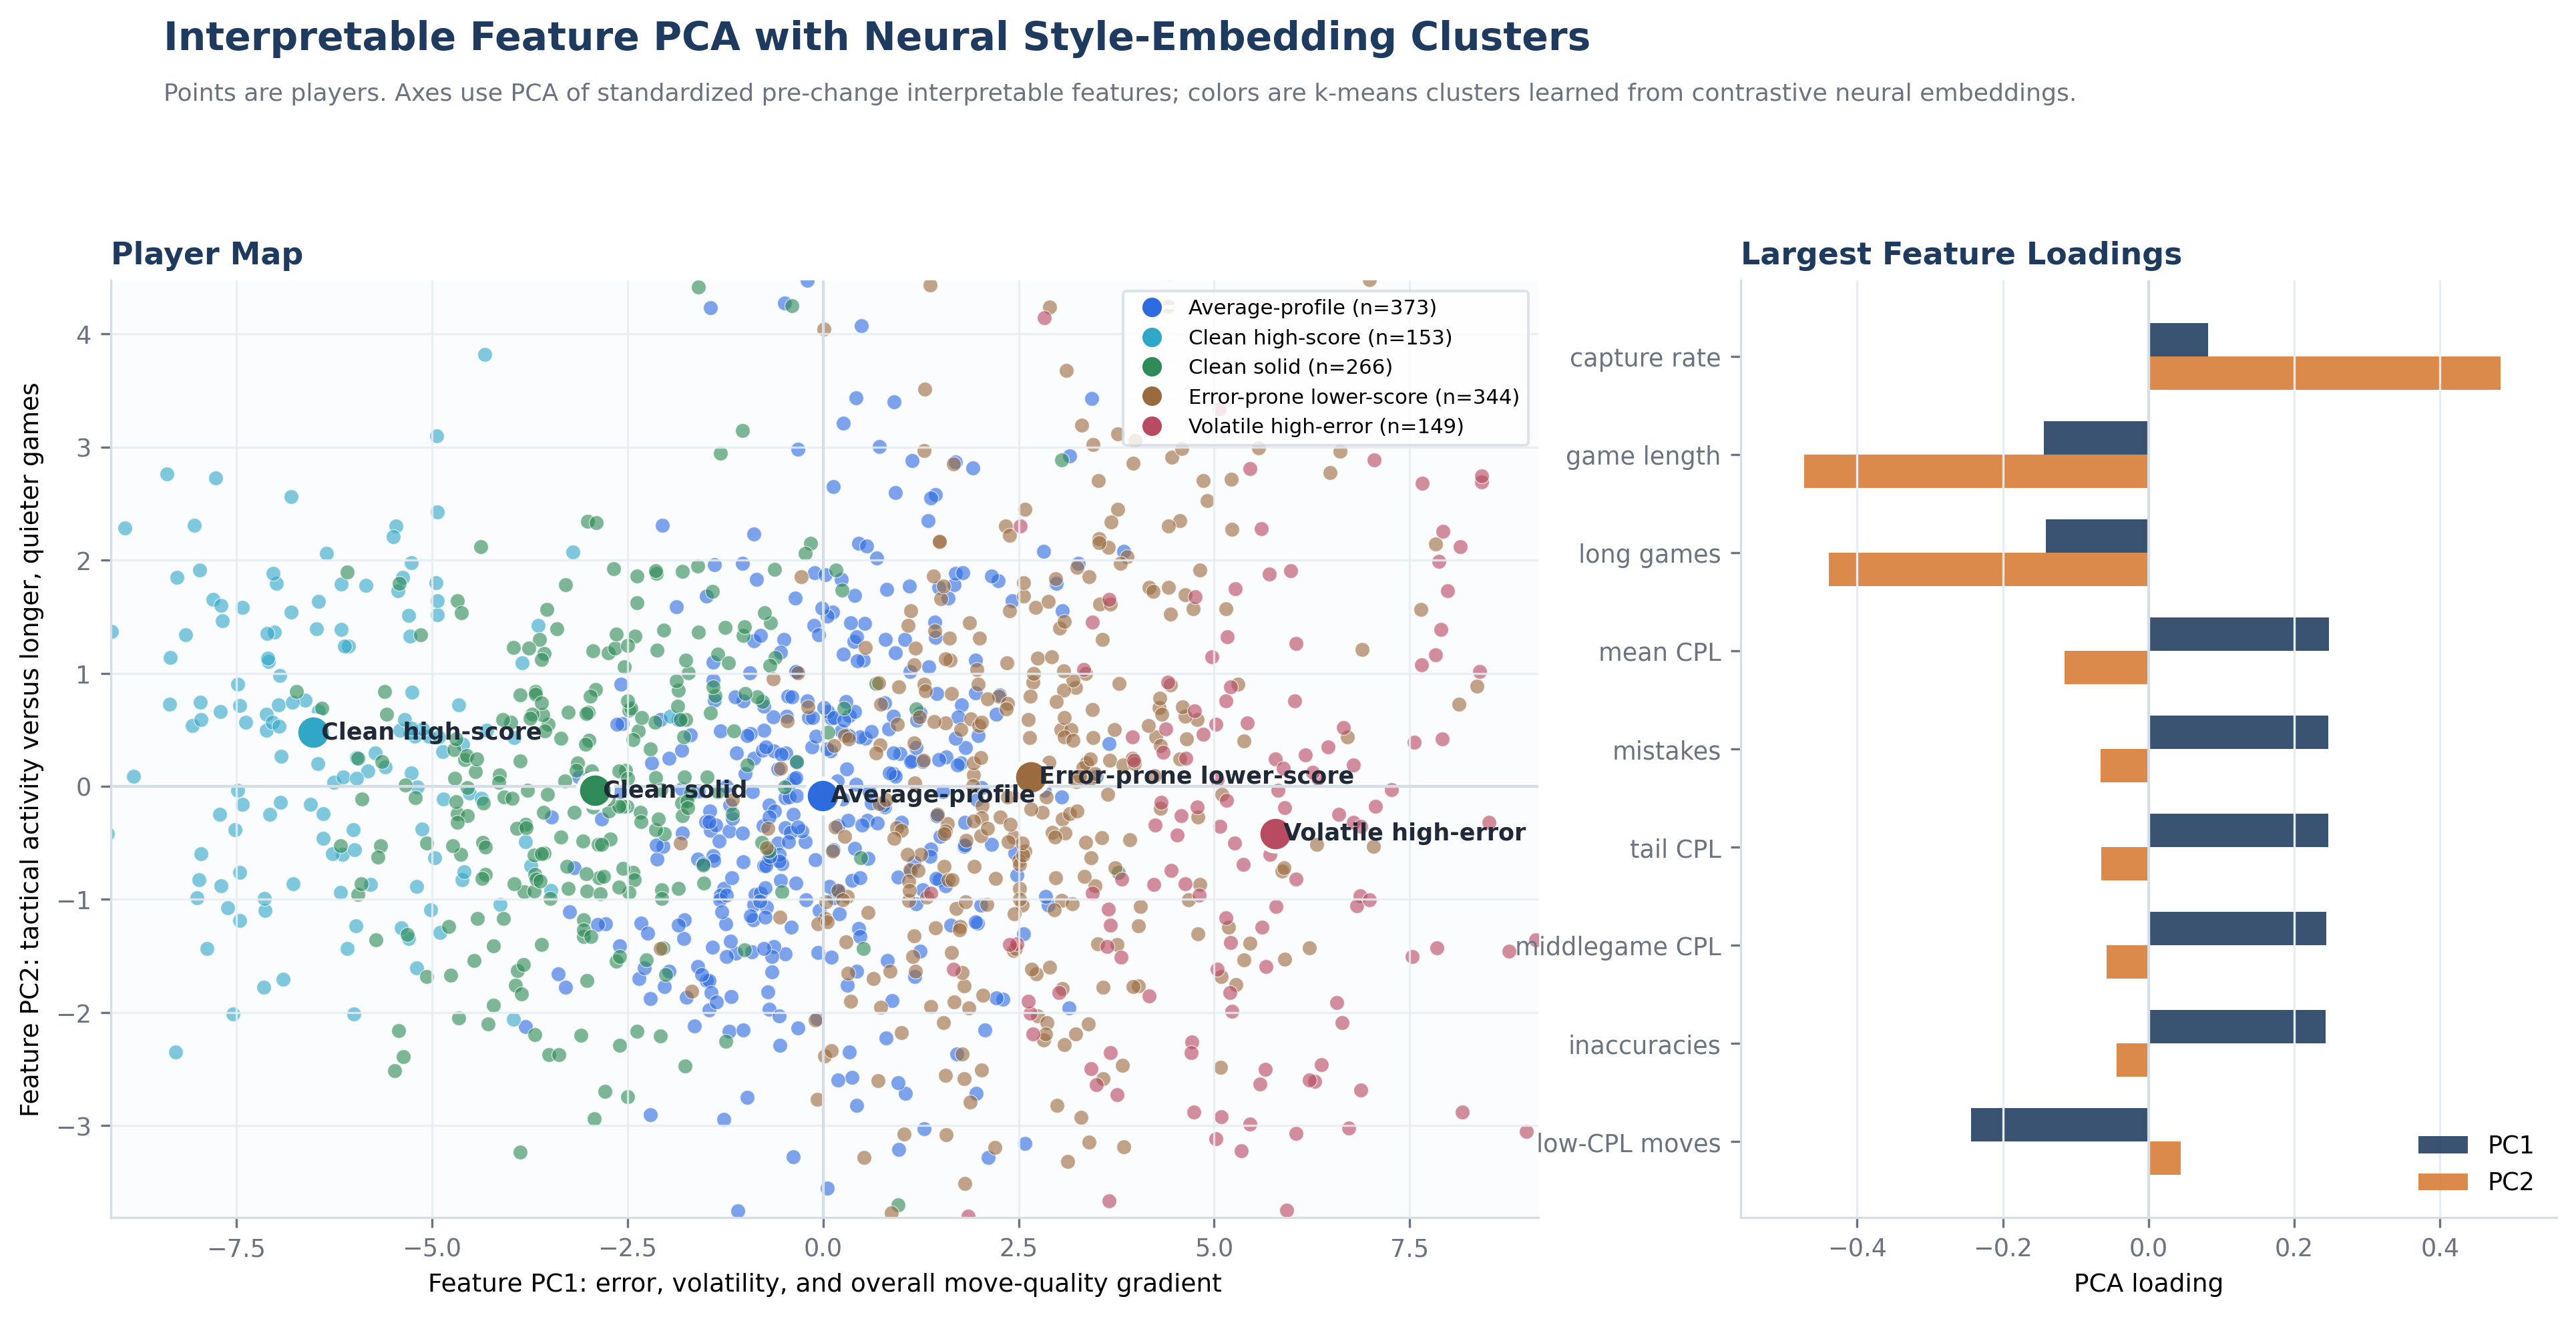
\includegraphics[width=\textwidth]{figures/figure11_interpretable_style_feature_pca.png}
\caption{Interpretable-feature PCA with neural style-embedding clusters. The axes are principal components of pre-change interpretable style features; the colors are clusters learned from contrastive neural player embeddings.}
\label{fig:style-feature-pca}
\end{figure}

\begin{table}[H]
\centering
\caption{Style Index Interactions}
\label{tab:style}
\begin{adjustbox}{max width=\textwidth}
\begin{tabular}{llrrrl}
\toprule
Model & Term & Estimate & SE & p-value & Unit \\
\midrule
Heavy-underdog result & Post \(\times\) chaos index & -0.0139 & 0.0053 & 0.009 & Per 1 SD chaos \\
Favorites-only result & Post \(\times\) chaos index & -0.0131 & 0.0056 & 0.020 & Per 1 SD chaos \\
Underdog triple model & Post \(\times\) chaos index & -0.0127 & 0.0057 & 0.025 & Per 1 SD chaos \\
Online-capital controls & Post \(\times\) chaos index & -0.0109 & 0.0051 & 0.034 & Per 1 SD chaos \\
Result over expected & Post \(\times\) chaos index & -0.0099 & 0.0047 & 0.035 & Per 1 SD chaos \\
Practical chaos model & Post \(\times\) practical chaos & -0.0107 & 0.0049 & 0.031 & Per 1 SD practical chaos \\
\bottomrule
\end{tabular}
\end{adjustbox}
\end{table}

This result rejects a plausible alternative story in which no-increment chess simply rewards practical chaos. The evidence points toward clean conversion and defensive stability as safer profiles after the reform. At the same time, the neural cluster results below show that the reform did not help only one narrow style group. All five neural style clusters improved their raw average accuracy after the switch; the difference is that chaotic profiles did not gain a relative score premium.

The neural style-embedding model is trained on player-game sequences from pre-change games only. Eligibility is defined using the full player-game panel: a player must have at least 100 total games and must appear both before and after the September 2025 rule change. This gives 1,295 eligible players in metadata, of whom 1,285 are matched to pre-change style features and usable move sequences. The sequence builder scans 805,256 PGN games, selects 519,945 pre-change games for eligible players, and writes 602,033 player-game sequences. To focus on style rather than memorized theory or forced late-game residues, the first 10 full moves and the last 10 plies are excluded. Sequences shorter than 12 moves are dropped and longer sequences are capped at 80 moves.

Each move token contains nine categorical fields: moved piece, origin square, destination square, capture indicator, check indicator, phase, binned centipawn loss, binned pre-move evaluation from the mover's perspective, and move-number bin. These tokens are passed through field embeddings, a feed-forward input layer, and a bidirectional GRU. The final hidden states are projected to a 64-dimensional normalized game embedding. The model is trained with a supervised contrastive loss: in each batch, two games from the same player are positives, while games from other players are negatives. The implementation uses 64 players per batch, two games per player, temperature 0.10, 10 percent within-player validation, and early stopping. Player embeddings are the averages of their pre-change game embeddings.

The averaged player embeddings are clustered with \(k\)-means. A grid over \(k=3,\ldots,8\) gives silhouette scores around 0.49 to 0.52; the five-cluster solution has a silhouette score of 0.497 and provides the most useful substantive granularity. The five clusters correspond to clean high-score players, clean solid players, average-profile players, error-prone lower-score players, and volatile high-error players.

\begin{figure}[H]
\centering
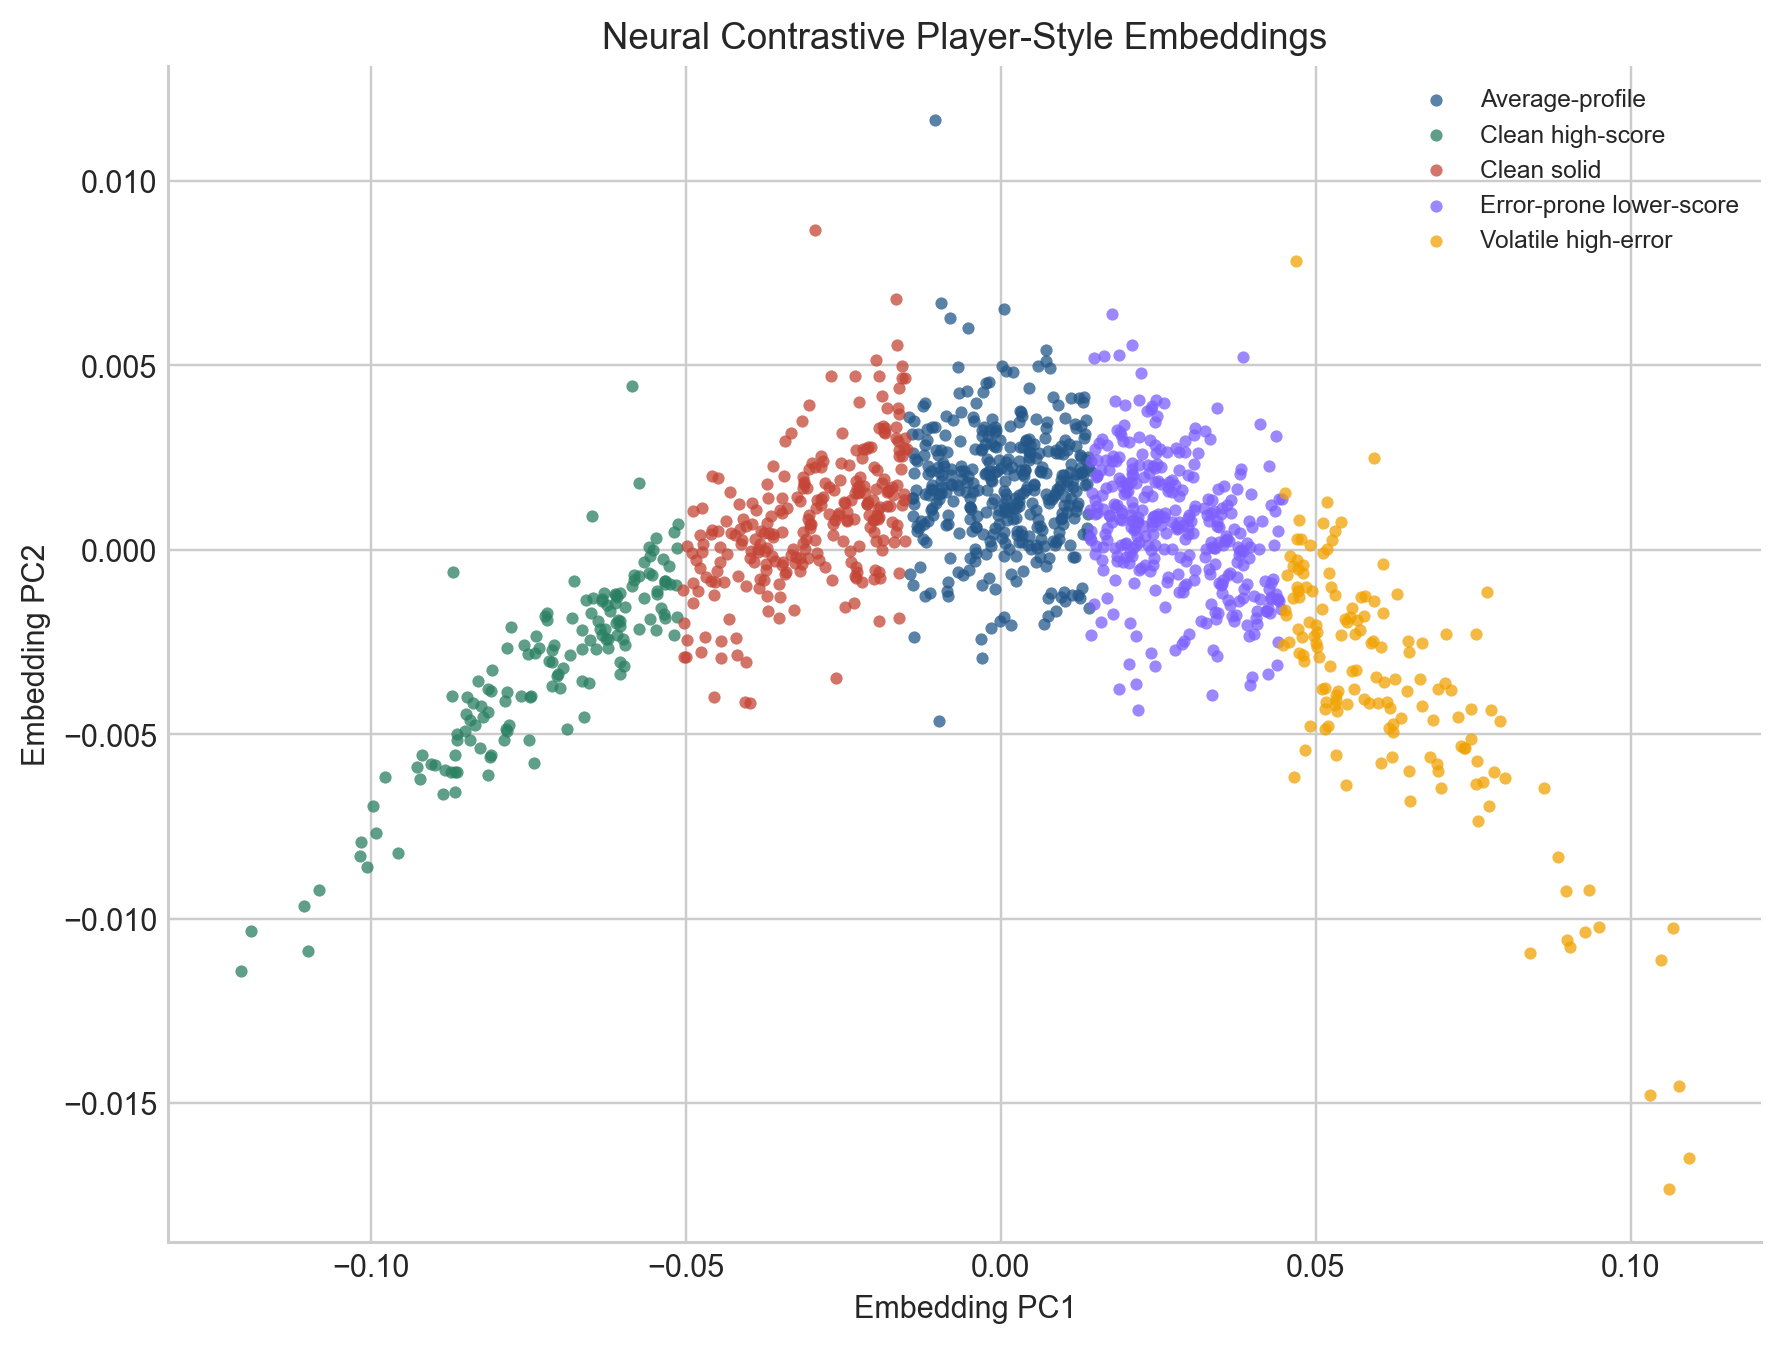
\includegraphics[width=0.85\textwidth]{figures/figure6_neural_style_cluster_map_static.png}
\caption{PCA of learned contrastive player embeddings. The plot shows the same five neural clusters in the two-dimensional projection of the 64-dimensional embedding space.}
\label{fig:neural-style}
\end{figure}

Table \ref{tab:neural-style-clusters} summarizes the cluster profiles. The clean high-score cluster is the strongest group ex ante: its average pre-change score share is 0.692, its mean centipawn loss is 28.4, and 57.3 percent of its pre-change games contain no player blunder. The clean solid cluster is less dominant in results but still low-error, with mean centipawn loss of 32.6 and a no-blunder-game rate of 46.0 percent. The average-profile cluster sits near the sample center. The error-prone lower-score and volatile high-error clusters have substantially higher centipawn loss, higher blunder rates, and lower pre-change score shares.

\begin{table}[H]
\centering
\caption{Neural Style-Embedding Cluster Profiles}
\label{tab:neural-style-clusters}
\begin{adjustbox}{max width=\textwidth}
\begin{tabular}{lrrrrrr}
\toprule
Cluster label & Players & Pre result & Mean CPL & No-blunder games & Accuracy delta & Result delta \\
\midrule
Clean high-score & 153 & 0.692 & 28.38 & 0.573 & 0.616 & -0.0216 \\
Clean solid & 266 & 0.579 & 32.60 & 0.460 & 0.752 & -0.0217 \\
Average-profile & 373 & 0.496 & 36.07 & 0.387 & 0.801 & -0.0176 \\
Error-prone lower-score & 344 & 0.421 & 39.38 & 0.336 & 0.711 & -0.0197 \\
Volatile high-error & 149 & 0.355 & 43.78 & 0.266 & 0.653 & -0.0176 \\
\bottomrule
\end{tabular}
\end{adjustbox}
\end{table}

The important result is that all five neural style clusters show positive raw accuracy changes after the reform, from about +0.62 to +0.80 Chess.com accuracy points on equal-player averages. This is informative because it rules out a simple story in which only clean or elite styles adjusted to the new time control. The broad accuracy improvement is consistent with the extra two minutes of initial time improving average move quality. The score-share deltas are small and mostly negative across clusters, which should not be interpreted as a causal style loss because the post-change tournament field, participation composition, and schedule changed at the same time. The causal style evidence therefore comes from the fixed-effect style-index regressions, while the neural embedding model contributes two things: it shows that pre-change move sequences contain stable player-style information, and it shows that the move-quality improvement after 5+0 was broad across learned style groups.

\subsection{Synthesis}

The robust results describe a coherent pattern. First, 5+0 increased returns to skill rather than randomness: rating advantages and accuracy advantages became more valuable. Second, the mechanism is conversion under constraint: stronger players converted advantages faster, lost fewer winning positions, recovered better from inferior positions, and avoided the style penalty associated with chaos. Third, the clock evidence shows why the constraint changed. Players had more initial time and less ordinary low-clock exposure, but severe time trouble became much more dangerous because the increment no longer insured recovery. Fourth, adaptability is heterogeneous: younger players, online specialists, and players with pre-change defensive or complexity-tolerance traits appear better positioned for the new format. Fifth, the tournament itself changed through selection: old late-slot regulars were hurt mainly through participation and completion, not through lower per-game move quality.

\section{Null, Weak, and Unsupported Results}

This section reports analyses that were implemented but did not produce robust evidence. These results are important because they rule out simple mechanisms that would otherwise be tempting explanations for the reform.

\subsection{Player and Game-Level Null Results}

\subsubsection{Broad Female-Status Effects}

The broad \(\text{Post} \times \text{Female}\) interaction is not robust for overall result or accuracy. Female-status interactions in late-round player-game models are also not statistically stable. A mixed-gender within-game score result is statistically strong: the female side lost about 2.6 percentage points of score share after the switch in mixed-gender games. However, this result is not matched by a clear accuracy effect and applies only to a selected subset of games. For this reason the thesis treats gender as a secondary heterogeneity result rather than a main headline.

\subsubsection{GDP and Resource Advantage}

The data do not support a robust conditional-performance effect of country GDP. Interactions between the post indicator and log GDP are not statistically clear for result or accuracy. Within-game GDP-gap models also do not produce robust performance differences. Country resources may matter for long-run chess development, training infrastructure, or participation selection, but the current Titled Tuesday panel does not show a clean post-change per-game performance effect.

\subsubsection{Country Local-Time Exposure}

Several country-time mechanisms were tested, including remaining-slot inconvenience, lost second-slot convenience, work-hour exposure, sleep-hour exposure, and seasonal time-zone burden. These variables do not robustly explain per-game result or accuracy after the reform. Some participation and rank-selection patterns appear for Asia/Oceania, but they are not strong enough to be treated as a main conditional-performance channel.

\subsubsection{White Advantage}

There is no robust evidence that the switch to 5+0 meaningfully changed White's advantage. This matters because one simple story would be that no-increment chess increases the payoff to opening initiative or first-move pressure. The data do not support that as a central mechanism.

\subsubsection{Generic FIDE Speed-Chess Specialization}

The evidence favors Chess.com-specific online capital rather than generic FIDE speed-chess specialization. FIDE blitz-over-classical and rapid-over-classical measures do not produce robust positive effects comparable to the Chess.com-over-classical gap. This distinction supports the interpretation that online platform skills matter, not only general faster-time-control chess ability.

\subsubsection{Close Games and Generic Decisiveness}

Game-level checks do not show that ex ante close games became generically more decisive or developed larger accuracy gaps. This rules out a broad chaos interpretation in which the new format simply makes close games more random. The stronger result is more specific: rating favorites convert better, and realized accuracy advantages translate more strongly into points.

\subsubsection{Consecutive Black Burden}

The consecutive-Black hypothesis is not supported at the clean per-game level. Interactions between the post indicator and Black streak variables are not statistically clear in the main specifications. Some exploratory final-outcome color-streak variables appear later in the research logs, but the main player-game evidence does not support a central consecutive-color mechanism.

\subsubsection{Learning-by-Doing After the Reform}

Raw post-change exposure bins look like players improve with repeated participation in 5+0. However, fixed-effect learning models do not support a positive learning-by-doing effect. In some specifications, the coefficient on post-change game number is negative for result. This likely reflects selection and repeated-entry composition rather than true within-player adaptation. The thesis therefore avoids claiming that players learned the new format quickly over the observed post-period.

\subsubsection{Hard Tournament Paths}

Harder tournament paths, measured by Buchholz or opponents' cumulative scores, are associated with worse outcomes. But placebo and pretrend tests show that this pattern is not cleanly tied to the September 2025 reform. The hard-path variables are useful as controls and descriptive tournament-sorting measures, but not as a main causal mechanism.

\subsubsection{Lagged Loss and Tilt}

Previous losses and unexpected losses affect next-game outcomes, which confirms that tilt or momentum exists in Titled Tuesday. The rule-change interactions, however, are mostly not robust. The evidence does not show that the 5+0 reform created a new tilt mechanism or strongly changed the next-game effect of previous losses.

\begin{table}[H]
\centering
\caption{Selected Null and Weak Results}
\label{tab:null-results}
\begin{adjustbox}{max width=\textwidth}
\begin{tabular}{lll}
\toprule
Area & Tested mechanism & Current conclusion \\
\midrule
Gender & Broad female post interaction & No robust overall result or accuracy effect \\
Country resources & GDP post interaction & No robust conditional performance effect \\
Country time zones & Lost-slot and local-time exposure & Weak for per-game outcomes \\
Color & White advantage under 5+0 & No meaningful post-change shift \\
Speed specialization & FIDE blitz/rapid gaps & Weaker than Chess.com-specific capital \\
Close games & Decisiveness and accuracy dispersion & No broad chaos result \\
Color streaks & Consecutive Black burden & Not supported in clean per-game models \\
Learning & Repeated post-change exposure & No clean positive learning effect \\
Tournament path & Buchholz and opponent path & Descriptive, not cleanly causal \\
Tilt & Lagged losses and upsets & Tilt exists, reform interaction weak \\
\bottomrule
\end{tabular}
\end{adjustbox}
\end{table}

\subsection{Move-Level Null Results}

\subsubsection{Opening Preparation}

Opening preparation was tested using Chess.com ECO information, book-exit move, evaluation at book exit, post-book accuracy, and pre-change opening specialization. These variables do not produce robust post-change interactions after multiple-testing adjustment. The current data therefore do not support the claim that 5+0 primarily increased returns to opening preparation.

This null result is useful because the reform plausibly could have rewarded memorized preparation: no increment makes early time savings valuable, and a five-minute base gives enough time for deeper prepared lines. The empirical evidence does not show that this mechanism dominates in the observed Titled Tuesday data.

\subsubsection{Simplification Strategy}

Simplification was measured using captures by move 20, queen-off indicators by moves 20 and 30, pieces remaining by move 30, material remaining by move 30, and a simplified-position indicator. The key hypotheses were that older players might simplify more after the switch and that simplification might protect them from the 5+0 penalty. These hypotheses are not robustly supported. Most interactions fail false-discovery adjustment, and the age-by-simplification interaction in result models is weak.

\subsubsection{Uniform Complex-Position Deterioration}

The complexity evidence is not a simple story that complex positions became worse for everyone. Some complexity interactions are statistically strong, but the signs indicate moderation by skill and age rather than a uniform increase in complex-position errors. The correct conclusion is that complexity changes the distribution of gains and losses under 5+0, not that all players make more errors in all complex positions.

\subsubsection{Error Cascades}

Error-cascade models tested whether a first blunder is more likely to be followed by another blunder or a higher next-five-move centipawn loss after the reform. These models do not produce robust post-change interactions for age, female status, or GDP. The main error-timing result is first-blunder timing, not post-blunder cascade behavior.

\subsubsection{Repeated Opponent Familiarity}

Repeated pairings are common enough to test whether prior meetings change move quality under the new format. Descriptively, repeated opponents have lower centipawn loss, but the post-change interaction terms are not robust. Prior meetings and prior directed score do not clearly reduce post-change blunder rates or centipawn loss in the Stockfish mechanism models.

\subsubsection{Female/Male Late and Critical-Position Mechanisms}

The female move-level interactions do not support a broad female-specific late or critical-position deterioration story. The interaction \(\text{Post} \times \text{Female} \times \text{CriticalEqual}\) is not robust, broad female blunder interactions are weak, and \(\text{Post} \times \text{Female} \times \text{Last10Ply}\) is negative in one model. The robust late and critical-position results are general and partly age-related, not clearly female-specific.

\subsubsection{Within-Game Accuracy Decay Slope}

For each player-game, an accuracy decay slope was estimated by regressing capped centipawn loss on move number. The post-by-age interaction is directionally interesting but has a q-value around 0.09. It is therefore not used as a headline result. Phase-specific late-game estimates and first-blunder timing provide stronger move-only evidence for within-game deterioration.

\subsubsection{Conversion Heterogeneity by Age and Female Status}

Conversion from winning positions by age and female status is suggestive but not robust after multiple-testing correction. The rating-advantage conversion result is strong; the age and female conversion interactions are not. The thesis therefore describes conversion technology mainly as a skill-premium mechanism rather than as an age or gender mechanism.

\subsection{Summary of Unsupported Mechanisms}

The null results sharpen the main interpretation. The reform does not appear to operate mainly through opening preparation, first-move advantage, GDP-based resource differences, broad gender effects, uniform complexity deterioration, simplification strategy, or error cascades. The supported mechanisms are more specific: higher returns to rating advantage, steeper accuracy-to-result conversion, late and critical-position costs, stronger conversion and defensive recovery by rating favorites, schedule-driven participation displacement, broad raw accuracy gains across neural style clusters, and negative relative score returns to chaotic pre-change style.

\section{Conclusion}

This thesis studies how a major online chess tournament reform changed the relationship between player characteristics, decision quality, and competitive outcomes. In September 2025, Chess.com changed Titled Tuesday from a 3+1 increment format with two weekly time slots to a 5+0 no-increment format with one main weekly slot. The reform created a useful empirical setting because it affected a repeated elite competition with stable player identities, objective ratings, complete game outcomes, and reconstructable move histories.

The strongest result is that the new format increased the return to relative skill. A 100-point rating advantage became worth about 1.2 additional percentage points of score share after the reform. This result survives the main robustness checks: excluding early rounds, restricting the window around the reform, using balanced players, adding paired-game fixed effects, and comparing against placebo cutoffs. The win/loss decomposition shows that stronger players won more and lost less, while draw probability changed little.

The second major result is that outcomes became more tightly linked to realized move quality. Accuracy advantages converted more strongly into points under 5+0. This is not interpreted as a causal effect of accuracy because accuracy is measured inside the game. Instead, it describes a steeper chess production function: given the same observed quality advantage over an opponent, the advantage was worth more in the no-increment format.

The move-level and clock analysis explains where this skill premium appears. Late-game and final-ten-ply errors increased under 5+0. Critical equal positions became more costly. Rating favorites converted winning positions more effectively, converted +2 positions faster, let fewer winning positions fall back to equality, and recovered more from -2 positions. Direct clock evidence sharpens the interpretation. Ordinary low-clock exposure became less common because players started with more time, but severe time trouble became more costly, recovery from low-clock states nearly disappeared, and opponent clock weakness became more valuable for conversion and defensive escape. Predetermined defensive skill and complexity tolerance predicted lower post-change errors. These results support a conversion-technology interpretation: 5+0 rewards players who can turn advantages into wins and survive worse positions under a different time-control technology.

Adaptability is heterogeneous. Younger players performed better relative to older players after the reform, although pretrend and placebo evidence require cautious causal language. Online-platform capital also mattered: players with high Chess.com ratings relative to classical ratings gained more, consistent with the value of interface fluency and online practical skill. Old late-slot regulars were harmed by the schedule component of the reform, but mainly through participation and completion margins rather than lower per-game accuracy.

The style analysis adds a data-science layer. Interpretable pre-change style indexes show that historically chaotic profiles did not receive a relative score premium from 5+0. If anything, chaos-creation style is associated with lower post-change score share. This rejects a plausible story that no-increment chess rewards practical chaos. The neural contrastive model shows that stable player-style embeddings can be learned from pre-change move sequences, and the resulting clusters align with meaningful chess profiles. All five neural style clusters show raw post-change accuracy improvements, so the neural result is not a null result: it shows that the move-quality gains from the new format were broad across learned styles, even though chaotic style did not become relatively more rewarded in score terms.

Several hypotheses were not supported. The data do not show robust effects for GDP, White advantage, broad female-status interactions, country local-time exposure, opening preparation, or simplification strategy. They also do not support uniform complex-position deterioration, repeated-opponent familiarity, or post-blunder error cascades as main channels. These null results are useful because they narrow the interpretation. The reform did not simply make chess more random, nor did it mostly reward openings or first-move initiative. It appears to have increased the value of skillful conversion and online adaptation while also changing who could participate consistently.

The main limitation is that the reform bundled the time-control change with the removal of the late slot and changes in the event's broader competitive cycle. The analysis separates conditional game performance from participation and completion, but the institutional shock is still multi-dimensional. A second measurement caveat is that clock annotations measure recorded remaining time, not psychological pressure directly. Premoves, interface latency, and online execution speed can affect the mapping between clock change and cognitive thinking time.

Future work could extend the thesis in three directions. First, the clock models could be combined with richer behavioral data on premoves, mouse speed, and interface latency to separate thinking time from execution time. Second, the neural style model could be extended from descriptive cluster comparisons to a full econometric treatment-heterogeneity design by estimating post-change style-cluster interactions with player and event fixed effects. Third, the tournament-selection part could be expanded into a structural participation model that separates time-zone costs, prize incentives, expected field strength, and player availability.

The overall empirical conclusion is that the Titled Tuesday reform changed both performance and selection. Conditional on playing, skill mattered more. In the move and clock data, that skill premium is visible in conversion, defensive recovery, late-game mistakes, critical positions, severe low-clock states, and the disappearance of increment insurance. In the tournament data, the single-slot design shifted participation and completion. The format change therefore reweighted elite online chess toward players who combine objective strength, online platform capital, and stable conversion under no-increment constraints.


\newpage
\bibliographystyle{plainnat}
\bibliography{references}

\newpage
\appendix
\section{Repository and Reproducibility Notes}

The thesis project is stored in the GitHub/Overleaf repository:

\begin{quote}
\url{https://github.com/ElijahSum/Master-Thesis-HSE}
\end{quote}

The current LaTeX project contains the following main files and folders:

\begin{itemize}
    \item \texttt{main.tex}: main LaTeX file;
    \item \texttt{sections/}: thesis section files;
    \item \texttt{references.bib}: bibliography;
    \item \texttt{figures/}: generated thesis figures;
    \item \texttt{tables/}: generated stargazer table outputs.
\end{itemize}

The public replication package is organized as a staged workflow. The main code folders are:

\begin{itemize}
    \item \texttt{code/01\_data\_collection/}: accuracy scraping, player metadata enrichment, and PGN fetching;
    \item \texttt{code/02\_data\_construction/}: final panel construction, Stockfish evaluation, clock features, move mechanisms, and style features;
    \item \texttt{code/03\_analysis/}: game-level, move-level, and clock-time econometric analysis;
    \item \texttt{code/04\_reporting/}: table and figure generation scripts;
    \item \texttt{code/05\_apps/}: optional opening-explorer application.
\end{itemize}

\section{Generated Tables and Figures}

The project contains stargazer-generated tables created by \path{../code/04_reporting/table_scripts/create_master_thesis_tables.R}. The LaTeX copies are stored in \texttt{tables/}:

\begin{itemize}
    \item \texttt{table1\_baseline\_game\_level\_effects.tex};
    \item \texttt{table2\_rating\_advantage\_robustness.tex};
    \item \texttt{table3\_time\_slot\_displacement.tex};
    \item \texttt{table4\_move\_mechanisms.tex};
    \item \texttt{table5\_style\_index\_interactions.tex};
    \item \texttt{table6\_null\_and\_weak\_results.tex}.
\end{itemize}

The figures were created by \texttt{../code/04\_reporting/figure\_scripts/create\_master\_thesis\_figures.py}. Static PNG figures are included in the thesis. The interactive Plotly neural cluster map is also stored as \texttt{figures/figure6\_neural\_style\_cluster\_map.html}.

Additional presentation figures for this thesis draft were created by \path{../code/04_reporting/figure_scripts/create_advanced_thesis_visuals.py}. These include the data architecture map, the rating-advantage robustness plot, the Stockfish mechanism dashboard, and the clean-outline evidence map. The interpretable style-feature PCA figure was created by \path{../code/04_reporting/figure_scripts/create_style_pca_figure.py}.

\section{Main Data Inputs}

The main player-game regression dataset is:

\begin{quote}
\path{data/final_regression_data_tournaments_2022_2026.csv}
\end{quote}

The two Stockfish centipawn-loss outputs used for the final move-level analysis are:

\begin{quote}
\path{outputs/whole_dataset_2022_2024/centipawn_loss_nodes2000_watch/centipawn_loss_watch.csv}
\end{quote}

\begin{quote}
\path{outputs/whole_dataset_2024_2026/centipawn_loss_nodes2000_watch/centipawn_loss_watch.csv}
\end{quote}

The PGN input used for the most recent move-data construction is:

\begin{quote}
\path{outputs/whole_dataset_2024_2026/whole_dataset_2024_2026.pgn}
\end{quote}

The current move-mechanism output uses a merged Stockfish and metadata sample of 27,517,197 usable move rows and 616,731 player-games.


\end{document}
